
\documentclass[a4paper]{article}\par \usepackage{style}\par 
\iffalse
\usepackage[euler-digits,euler-hat-accent, OT1]{eulervm}
\usepackage[mathscr, mathcal]{eucal}
\fi\par \title{Complementi di Matematica - Esercitazioni}
\author{Alessandro Piazza\thanks{alessandro.piazza@sns.it}}\par \begin{document}\par \maketitle\par \clearpage\par \begin{abstract}
	Questa è una raccolta di esercizi e problemi per il corso di Complementi di Matematica del primo anno della Scuola Normale Superiore (Fulvio Ricci, Simone di Marino, Andrea Mennucci) per mio bisogno come supporto allo studio. La maggior parte delle soluzioni sono state trascritte da quelle date a lezione o sono state scritte da me, ma anche altri allievi del mio anno hanno contribuito. Sono quindi ben accette segnalazioni di errori, sia typo che concettuali. \\
	I testi degli esercizi sono ad opera di Simone di Marino (capitoli 1-12), Ugo Bindini (Appendice A), Andrea Mennucci (\emph{Database di Esercizi per corso Matematica I anno} e capitoli 9-18) e Carlo Mantegazza (\emph{Complementi di matematica - I anno SNS 2013/14. Esercizi}). Nell'Appendice A sono riportati i testi di alcuni esercizi dei compiti scritti ad opera dei docenti del corso dell'anno del compito. \\
	\ \\
	Quest'opera è stata rilasciata con licenza Creative Commons Attribuzione - Condividi allo stesso modo 4.0 Internazionale. Per leggere una copia della licenza visita il sito web \url{http://creativecommons.org/licenses/by-sa/4.0/}. \href{http://creativecommons.org/licenses/by-sa/4.0/}{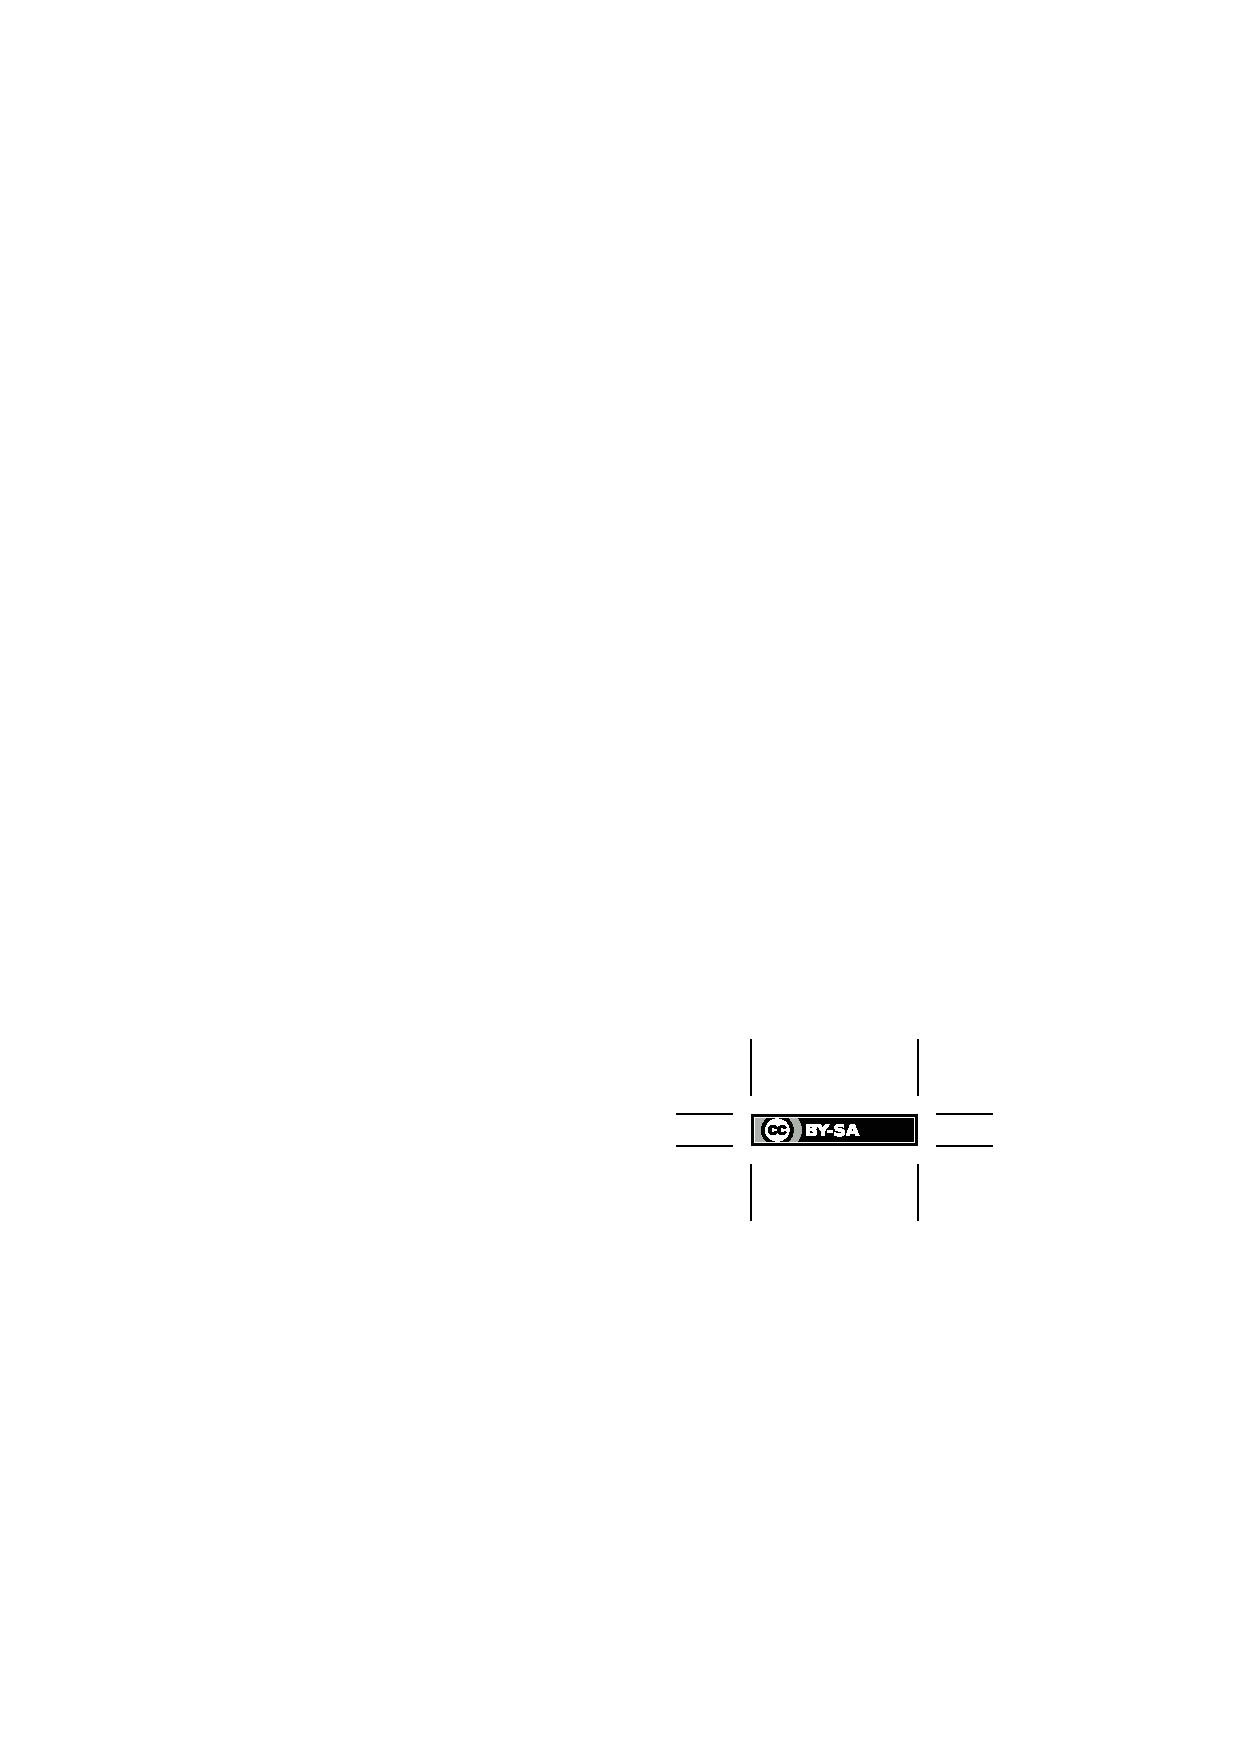
\includegraphics[scale = 0.5]{by-sa}}
\end{abstract}\par \tableofcontents\par \clearpage\par 
\section{Logica e teoria degli insiemi}
\begin{es}
  Dimostrare le seguenti identità insiemistiche dove gli insiemi che compaioni sono tutti sottoinsiemi di $ X $
  \begin{enumerate}
  \item $ (A^c)^c = A $
  \item $ (A \cup B)^c = A^c \cap B^c $ e $ (A \cap B)^c = A^c \cup B^c $
  \item $ (A_1 \cup A_2) \cap B = (A_1 \cap B) \cup (A_2 \cap B) $ e $ (A_1 \cap A_2) \cup B = (A_1 \cup B) \cap (A_2 \cup B) $
  \item $ \bigcup_{i \in I} A_i ^c = \left (\bigcap_{i \in I} A_i \right )^c $ e $ \bigcap_{i \in I} A_i ^c = \left (\bigcup_{i \in I} A_i \right )^c $
  \item $ \left (\bigcup_{i \in I} A_i \right ) \cap B = \bigcup_{i \in I} (A_i \cap B) $ e $ \left (\bigcap_{i \in I} A_i \right ) \cup B = \bigcap_{i \in I} (A_i \cup B) $
  \item Qual è una possibile espressione per $ \left (\bigcap_{i \in I} A_i \right ) \cup \left (\bigcap_{j \in J} B_j \right ) $?
  \end{enumerate}
\end{es}
Per ognuno dei punti risolviamo solo  la prima parte. In quasi tutti i punti useremo in modo implicito l'Assioma di estensionalità per mostrare uguaglianze tra insiemi
\begin{enumerate}
\item $ x \in (A^c)^c \iff x \notin A^c \iff \neg (x \in A^c) \iff \neg (x \notin A) \iff \neg(\neg(x \in A)) \iff x \in A $.
\item $ x \in (A \cup B)^c \iff x \notin A \cup B \iff \neg (x \in A \cup B) \iff \neg(x \in A \vel x \in B) \iff x \notin A \wedge x \notin B \iff x \in A^c \wedge x \in B^c \iff x \in A^c \cap B^c $.
\item $ x \in (A_1 \cup A_2) \cap B \iff x \in (A_1 \cup A_2) \wedge x \in B \iff (x \in A_1 \vel x \in A_2) \wedge x \in~B \iff (x \in A_1 \wedge x \in B) \vel (x \in A_2 \wedge x \in B) \iff (x \in A_1 \cap B) \vel (x \in A_2 \cap B) \iff x \in (A_1 \cap B) \cup (A_2 \cap B) $.
\item $ x \in \bigcup_{i \in I} A_i ^c \iff \exists i \in I : x \in A_i^c \iff \exists i \in I : \neg (x \in A_i) \iff \neg (\forall i \in I : x \in A_i) \iff \neg \left(x \in \bigcap_{i \in I} A_i \right) \iff x \notin \bigcap_{i \in I} A_i \iff x \in \left(\bigcap_{i \in I} A_i \right)^c $.
\item $ x \in \left (\bigcup_{i \in I} A_i \right ) \cap B \iff x \in \bigcup_{i \in I} A_i \wedge x \in B \iff (\exists i \in I : x \in A_i) \wedge x \in B \iff \exists i \in I : (x \in A_i \wedge  x \in B) \iff x \in \bigcup_{i \in I} (A_i \cap B) $
\item $ x \in \left (\bigcap_{i \in I} A_i \right ) \cup \left (\bigcap_{j \in J} B_j \right ) \iff x \in \bigcap_{i \in I} A_i \vel x \in \bigcap_{j \in J} B_j \iff (\forall x \in I : x \in A_i) \vel (\forall j \in J : x \in B_j) \iff \forall i \in I, \forall j \in J : x \in A_i \vel x \in B_j \iff \forall i \in I, \forall j \in J : x \in A_i \cup B_j \iff x \in \bigcap_{\substack{i \in I \\ j \in J}} A_i \cup B_j $. \\
  Concludiamo pertanto che $ \left (\bigcap_{i \in I} A_i \right ) \cup \left (\bigcap_{j \in J} B_j \right ) = \bigcap_{\substack{i \in I \\ j \in J}} (A_i \cup B_j) $.
\end{enumerate}\par \begin{es}
  Ricordiamo che $ A \Delta B = (A \cup B) \setminus (A \cap B) $. Mostrare che
  \begin{enumerate}
  \item $ A \Delta B = (A \setminus B) \cup (B \setminus A) $
  \item $ (A \Delta B) \Delta C = A \Delta (B \Delta C) $
  \end{enumerate}
  È sempre vero che $ A \Delta B \Delta C = (A \Delta B) \cap (B \Delta C) \cap (C \Delta A) $?
\end{es}\par \begin{es}
  Mostrare che $ A \times B \subseteq \P(\P(A \cup B)) $. Dedurne che se $ n \in \N $ allora $ 2^{2^n} \leq n^2 $.
\end{es}
Per definizione $ A \times B $ è l'insieme delle coppie ordinate $ (a, b) $ al variare di $ a \in A $ e di $ b \in B $. Formalmente la coppia ordinata viene definita come un insieme nel modo seguente \[(a,b) = \{\{a\}, \{a, b\}\}.\] \textsf{Intuitivamente $ \P(A \cup B) $ contiene i sottoinsiemi di $ A \cup B $ tra cui quindi anche $ \{a\} $ e $ \{a,b\} $; allora $ \P(\P(A \cup B)) $ conterrà anche l'insieme $ \{\{a\}, \{a, b\}\} $. Poiché quindi ogni elemento di $ A \times B $ è anche in $ \P(\P(A \cup B)) $ deduciamo che $ A \times B \subseteq \P(\P(A \cup B)) $.}\\
Tale relazione si traspone alle cardinalità nella disuguaglianza $ |A \times B| \leq |\P(\P(A \cup B))| $. Allora se prendiamo $ A = B $ tale che $ |A| = n $, con $ n \in \N $, segue banalmente che $ n^2 \leq 2^{2^n} $.\par 
\begin{es}
  \textsf{ATTENZIONE : non l'ho capito bene, molto probabilmente $ x $ e $ y $ sono scambiati.} \\
  L'Assioma di buona fondazione afferma che ogni insieme $ x $ non vuoto contiene un elemento disgiunto da $ x $ stesso. In simboli \[\forall x, \ \exists y : (y \in x) \wedge (y \cap x = \emptyset).\] Dimostrare che
  \begin{enumerate}
  \item non può esistere un insieme $ x $ tale che $ x \in x $;
  \item non possono esistere $ x_1, \dots, x_n $ insiemi tali che $ x_1 \in x_2 \in \dots \in x_n \in x_1 $;
  \item non possono esistere $ x_n $ insiemi con $ n \in \N $ tali che $ x_{n+1} \in x_{n} $.
  \end{enumerate}
\end{es}
Procediamo per assurdo: per ognuono dei punti supporremo vera la richiesta e mostreremo che ciò conduce ad una negazione dell'assioma ovvero \[\neg (\forall x, \ \exists y : (y \in x) \wedge (y \cap x = \emptyset)) \iff \exists x, \ \forall y : (y \notin x) \vel (y \cap x \neq \emptyset). \]
\begin{enumerate}
\item Sia $ x \neq \emptyset $ tale che $ x \in x $ e definiamo $ y = \{x\} $ che esiste per l'\textsc{Assioma della coppia}. Tale insieme soddisfa la negazione dell'assioma in quanto $ x \in \{x\} $ e, per ipotesi, $ x \in x $ dunque $ y \cap x = x \neq \emptyset $. Ciò è dunque assurdo e concludiamo quindi che $ \nexists x \neq \emptyset : x \in x $.
\item Siano $ x_1, \dots, x_n $ insiemi non vuoti tali che $ x_1 \in x_2 \in \dots \in x_n \in x_1 $ e consideriamo  $ y = \{x_n, \dots, x_2, x_1\} $. Allora $ y \neq \emptyset $ e per ogni $ 1 \leq k \leq n $ si ha $ x_k \cap y = \{x_n, \dots, x_1\} \neq \emptyset $, che contraddice l'assioma. D'altro canto gli $ x_1, \dots, x_n $ sono tali che per ogni $ k $, $ x_k \in x_k $, che è assurdo per quanto dimostrato al punto precendente.
\item Supponiamo che esiste una sequenza $ x_n $ di insiemi non vuoti, con $ n \in \N $ tale che $ x_{n+1} \in x_n $ e definiamo per ogni $ n $ $ y_n = \{x_n\} $ che esiste per l'\textsc{Assioma della coppia}. Allora $ y_n $ è un insieme non vuoto e $ y_n \cap x_n \neq \emptyset $ in quanto $ x_{n+1} \in x_n $, per ipotesi, e $ x_{n+1} \in y $. Ciò è assurdo in quanto contraddice l'assioma; concludiamo quindi che non possono esistere una successione infinita discendente di insiemi.
\end{enumerate}\par \section{Relazioni e funzioni}
\begin{es}
  Sia $ (T, \leq) $ un insieme totalmente ordinato e $ X $ un insieme. Data una famigli di inisemi $ \{A_t\}_{t \in T} $ con $ A_i \subset X $, si definiscano $ B_t = \bigcap_{s \geq t} A_s $, $ C_t = \bigcup_{s \geq t} A_s $ e successivamente \[\limsup_{t \in T} A_t = \bigcup_{t \in T} B_t \qquad \liminf_{t \in T} A_t = \bigcap_{t \in T} C_t.\]\\
  Si mostri che
  \begin{enumerate}
  \item la funzione $ f \colon (T, \leq) \to (\P(X), \subseteq) $ tale che $ f(t) = B_t $ è crescente e che $ g \colon (T, \leq) \to (\P(X), \subseteq) $ tale che $ g(t) = C_t $ è decrescente;
  \item $ (\limsup_{t \in T} A_t^1) \cup (\limsup_{t \in T}A_t^2) \subseteq \limsup_{t \in T} (A_t^1 \cup A_t^2) $;
  \item $ \limsup_{t \in T} (A_t^1 \cap A_t^2) \subseteq (\limsup_{t \in T} A_t^1) \cap (\limsup_{t \in T}A_t^2) $;
  \item $ \liminf_{t \in T} A_t^c = (\limsup_{t \in T} A_t)^c $;
  \item $ \limsup_{t \in T} A_t \subseteq \liminf_{t' \in T} A_{t'} $;
  \item se $ T $ ha massimo allora $ \limsup_{t \in T} A_t = \liminf_{t \in T} A_t $.
  \end{enumerate}
  Fornire, se esiste, un esempio dove $ \limsup_{t \in T} A_t \neq \liminf_{t \in T} A_t $. Nel caso in cui $ T = \N $, come si possono definire a parole $ \liminf $ e $ \limsup $ di famiglie di insiemi?
\end{es}\par 
Mostriamo prima i seguenti risultati che ci saranno utili nella risoluzione dell'esercizio\par \begin{lemma}
  Vale $ \bigcap_{i \in I \cup J} A_i = \left (\bigcap_{i \in I} A_i \right ) \cap \left (\bigcap_{i \in J} A_i \right ) $. Formula analoga vale per le'unione.
\end{lemma}
\begin{proof}
  Mostriamo l'uguaglianza insiemistica facendo uso dell'Assioma di estensionalità.
  \begin{align*}
    x \in \bigcap_{i \in I \cup J} A_i \iff (\forall i : (i \in I \cup J) \Rightarrow x \in A_i ) \iff (\forall i : (i \in I \vel i \in J) \Rightarrow x \in A_i ) \\
    x \in \left (\bigcap_{i \in I} A_i \right ) \cap \left (\bigcap_{i \in J} A_i \right ) \iff  (\forall i : (i \in I) \Rightarrow x \in A_i) \wedge (\forall i : (i \in J) \Rightarrow x \in A_i)
  \end{align*}
  Le due ultime proposizioni logiche sono in realtà equivalenti, ricordando infatti la definizione di implicazione $ (a \Rightarrow b) \iff (\neg a) \vel b $, si ha
  \[((p \vel q) \Rightarrow r) \iff (\neg (p \vel q)) \vel r \iff (\neg p \wedge \neg q) \vel r \iff (\neg p \vel r) \wedge (\neg q \vel r) \iff (p \Rightarrow r) \wedge (q \Rightarrow r) \qedhere\]
\end{proof}\par \begin{lemma}
  Vale $ \forall i \in I : A_i \subseteq B_i \Rightarrow \bigcup_{i \in I} A_i \subseteq \bigcup_{i \in I} B_i $. Regola analoga vale per l'intersezione e dunque anche per l'uguaglianza.
\end{lemma}
\begin{proof}
  Sia $ x \in A_i $. Per ipotesi sappiamo che $ \forall i \in I: (x \in A_i) \Rightarrow (x \in B_i) $. Ma allora se $ y \in \bigcup_{i \in I} A_i $ vuol dire che $ \exists i \in I : y \in A_i $ e quindi per ipotesi $ \exists i \in I : y \in B_i $, ovvero $ (y \in \bigcup_{i \in I} A_i) \Rightarrow (y \in \bigcup_{i \in I} B_i)  $ da cui segue la tesi per definizione di inclusione.
\end{proof}\par \begin{lemma}
  Vale $ 	(A_1 \subseteq B) \wedge (A_2 \subseteq B) \Rightarrow (A_1 \cup A_2) \subseteq B $.
\end{lemma}
\begin{proof}
  Se $ x \in A_1 $ allora in particolare è anche in $ A_1 \cup A_2 $ e quindi per ipotesi è in $ B $; se $ y \in A_2 $ allora in particolare è anche in $ A_1 \cup A_2 $ e quindi per ipotesi è in $ B $. Dunque ogni elemnto di $ A_1 \cup A_2 $ è in $ B $.
\end{proof}\par Passiamo quindi all'esercizio.
\begin{enumerate}
\item Per mostrare che $ f(t) $ è crescente dobbiamo verificare che $ \forall m, n \in T : m \leq n \Rightarrow B_m \subseteq B_n $. Si ha infatti \[B_m = \bigcap_{s \geq m} A_s = \left( \bigcap_{s \geq n} A_s \right ) \cap \left( \bigcap_{n > s \geq m} A_s \right ) = B_n \cap \left( \bigcap_{n > s \geq m} A_s \right ) \] dove il secondo passaggio è giustificato per il \textsc{Lemma 2.1}. Concludiamo quindi che $ B_m \subseteq B_n $ e dunque che $ f $ è crescente. \\
  Dimostrazione analoga vale per $ g(t) $.
\item Riscriviamo la tesi passando pe la definizione di $ \limsup $. Vogliamo mostrare quindi che \[\bigcup_{t \in T} B_t^1 \cup \bigcup_{t \in T} B_t^2 \subseteq \bigcup_{t \in T} B_t^{*}\] dove abbiamo definito $ B_t^{*} = \bigcap_{s \geq t} (A_t^1 \cup A_t^2) $. In virtù del \textsc{Lemma 2.2} sarà sufficiente mostrare che $ \forall t \in T $ vale $ B_t^1 \cap B_t^2 \subseteq B_t^{*} $, ovvero passando alla definizione di $ B_t $ equivale a mostrare che $ \forall t \in T $ vale \[\bigcap_{s \geq t} A_s^1 \cup \bigcap_{s \geq t} A_s^2 \subseteq \bigcap_{s \geq t} (A_s^1 \cup A_s^2).\] Sfruttando il \textsc{Lemma 2.3} ci basta mostrare che \[\bigcap_{s \geq t} A_s^1 \subseteq \bigcap_{s \geq t} (A_s^1 \cup A_s^2)\] \[\bigcap_{s \geq t} A_s^2 \subseteq \bigcap_{s \geq t} (A_s^1 \cup A_s^2)\] che sono sempre verificate in quanto $ \forall s \; A_s^1 \subseteq (A_s^1 \cup A_s^2) $ (analogo per $ A_s^2 $) e tale relazione passa all'intersezione per quanto dimostrato nel \textsc{Lemma 2.2}. Ripercorrendo le implicazioni appena mostrare concludiamo dunque che \[(\limsup_{t \in T} A_t^1) \cup (\limsup_{t \in T}A_t^2) \subseteq \limsup_{t \in T} (A_t^1 \cup A_t^2).\]
\item Per l'intersezione la dimostrazione analoga (\textsf{si sviluppanpo le definizioni e usando lemma 2.2 e lemma 2.3 ci si rionduce ad inclusioni ovvie}).
\item Passando alla definizione di $ \liminf $ e $ \limsup $ dobbiamo mostrare che \[\bigcap_{t \in T} C_t^{*} = \left (\bigcup_{t \in T} B_t \right )^c = \bigcap_{t \in T} B_t^{c}\] dove $ C_t^{*} = \bigcup_{t \in T} A_t^c $ e nell'ultima uguaglianza abbiamo usato la formula di \textsc{De Morgan}. Per il \textsc{Lemma 2.2} ci basta mostare quindi che $ C_t^{*} = B_t^c $ ovvero, usando la definizione \[\bigcup_{t \in T} A_t^c = \left (\bigcap_{t \in T} A_t \right )^c = \bigcup_{t \in T} A_t^{c}\] dove abbiamo fatto nuovamente uso delle formule di De Morgan. L'ultima relazione è sempre verificata e concludiamo quindi che \[\liminf_{t \in T} A_t^c = (\limsup_{t \in T} A_t)^c.\]
\item Prima di tutto mostriamo che si ha \[\bigcap_{s \geq t} A_s \subseteq \bigcup_{s \geq t'} A_s.\] Sia infatti $ x \in \bigcap_{s \geq t} A_s $, ovvero $ \forall s \in T : s \geq t \Rightarrow x \in A_s $: se $ t' \geq t $, siccome per $ s \geq t $ si ha $ x \in A_s $ basterà prendere $ s \geq t' \geq t $ e si avrà $ x \in \bigcup_{s \geq t'} A_s  $ (in quanto $ \exists s \in T: s \geq t' \Rightarrow x \in A_s $); se invece $ t \geq t' $ basterà prendere $ s \geq t \geq t' $ e si avrà $ x \in \bigcup_{s \geq t'} A_s  $.\\
  Ma allora per definizione si ha che $ \forall t \in T , \forall t' \in T $ si ha $ B_t \subseteq C_t' $ da cui deduciamo banalmente che $ \forall t \in T $ \[B_t \subseteq \bigcap_{t' \in T} C_t\] che per il \textsc{Lemma 2.2} implica che \[\bigcup_{t \in T} B_t \subseteq \bigcap_{t' \in T} C_t\] che è equivalente alla tesi \[\limsup_{t \in T} A_t \subseteq \liminf_{t' \in T} A_{t'}.\]
\item Sia $ t_0 = \max T $. Allora per $ \forall t \in T $ si ha \[B_t = \bigcap_{s \geq t} A_s \subseteq A_{t_0} \quad \mathrm{e} \quad C_t = \bigcup_{s \geq t} A_s \supseteq A_{t_0}.\] Inoltre poiché risulta $ B_{t_0} = \bigcap_{s \geq t_0} A_s = A_{t_0} $ e i $ B_t $ sono una famiglia di insiemi crescenti e ordinati per inclusione (per quanto mostrato nel punto 1) risulta $ \limsup_{t \in T} A_t = \bigcup_{t \in T} B_t = B_{t_0} = A_{t_0} $. D'altro canto risulta $ C_{t_0} = \bigcup_{s \geq t_0} A_s = A_{t_0} $ e i $ C_t $ sono una famiglia di insiemi decrescenti e ordinati per inclusione (per quanto dimostrato al punto 1); pertanto $ \liminf_{t \in T} A_t = \bigcap_{t \in T} C_t = C_{t_0} = A_{t_0} $. Concludiamo quindi che se $ T $ ha massimo $ t_0 $ si ha \[\limsup_{t \in T} A_t = \liminf_{t \in T} A_t = A_{t_0}\]
\end{enumerate}
Nel caso di $ T = \N $ possiamo definire a parole
\begin{align*}
  \limsup_{n \in \N} A_n & = \{\text{gli $ x $ che sono definitivamente in $ A_n $}\} = \\
                         & = \{x \in X : \exists n_0 : \forall n \geq n_0 \; x \in A_n\} \\
                         & \\
  \liminf_{n \in \N} A_n & = \{\text{gli $ x $ che sono frequentemente in $ A_n $}\} = \\
                         & = \{x \in X : \forall n_0 : \exists n \geq n_0 \; x \in A_n\}\\
\end{align*}\par \textcolor{red}{Hint Bindini -  Le definizioni sono scambiate rispetto alla consueta definizione per numeri reali, infatti si vede dal risultato del punto 5. Per costruire esempi simili a quelli delle successioni ragiona così: qual è la caratteristica importante della successione $ (-1)^n $? Il fatto che $ -1 < +1 > -1 < +1 > \ldots $ Qui però la relazione d'ordine non è $ < $ dei numeri reali, bensì "contenuto" degli insiemi. Quindi cerca di costruire $ \{A_n\} $ tali che $ A_1 < A_2 > A_3 < A_4 > \ldots $ (dove "$ < $" sta per il contenimento) e poi verificare\ldots}\par 
\begin{es}
  Un medagliere olimpico può essere considerato come una collezione di tre funzioni $ o, a, b \colon S \to \N $, dove $ S $ è l'insieme delle nazioni e $ o(s) $, $ a(s) $ e $ b(s) $ sono rispettivamente gli ori, gli argenti e i bronzi olimpici. Vorremmo ora stabilire un possibile ordine tra le nazioni; per fare ciò immaginiamo di avere due principi che devono essere sicuramente veri:
  \begin{enumerate}[label=(\roman*)]
  \item Se una nazione $ s_1 $ ha sia più ori, che più argenti che più bronzi, di una nazione $ s_2 $ allora necessariamente $ s_1 $ dovrà stare più alta in classifica di $ s_2 $.
  \item Se una nazione $ s_1 $ ha un bronzo in meno di $ s_2 $ ma un argento in più e lo stesso numero di ori allora necessariamente $ s_1 $ dovrà stare più alta in classifica di $ s_2 $ (stesso dicasi per un argento in meno ma un oro in più).
  \end{enumerate}
  Stabiliremo quindi che una nazione $ s_1 $ è necessariamente più alta in classifica di $ s_2 $ se posso raggiungere la configurazione di medaglie di $ s_1 $ dalla configurazione di $ s_2 $ compiendo solo operazioni di tipo (i), cioè addizioni di medaglie, o di tipo (ii), cioè miglioramento delle medaglie. Mostrare che questo accade se e solo se $ (o(s_1), a(s_1), b(s_1)) \succeq (o(s_2), a(s_2), b(s_2)) $ dove $ (\N^3, \succeq) $ è la relazione d'ordine definita come
  \[(a, b, c) \succeq (a', b', c') \liff
    \begin{cases*}
      a \geq a' \\
      a + b \geq a' + b' \\
      a + b + c \geq a' + b' + c' \\
    \end{cases*}\]
  Mostrare che questa è effettivamente una relazione d'ordine e che non è totale. Qual è la relazione d'ordine usata normalmente nel definire la classifica nel medagliere? Essa è totale?
\end{es}
Dobbiamo mostrare che si ha $ s_1 \geq s_2 \iff (o(s_1), a(s_1), b(s_1)) \succeq (o(s_2), a(s_2), b(s_2)) $; per fare ciò verifichiamo le due implicazioni
\begin{itemize}[label=$ \Rightarrow $]
\item Se la (i) è verificata possiamo scrivere che
  \[\begin{cases*}
      o(s_1) \geq o(s_2) \\
      a(s_1) \geq a(s_2) \\
      b(s_1) \geq b(s_2) \\
    \end{cases*}\]
  Sommando la prima alla seconda e la nuova seconda alla terza otteniamo esattamente il sistema che definisce la relazione $ \succeq $ e concludiamo quindi che $ (o(s_1), a(s_1), b(s_1)) \succeq (o(s_2), a(s_2), b(s_2)) $. Se invece si ha $ o(s_1) = o(s_2) $, $ a(s_1) = a(s_2) + 1 $ e $ b(s_1) = b(s_2) - 1 $ ???
\end{itemize}
\begin{itemize}[label=$ \Leftarrow $]
\item ???
\end{itemize}
Verifichiamo ora che la relazione $ \succeq $ è effettivamente un relazione d'ordine
\begin{itemize}
\item \emph{Riflessiva}: $ \forall (a, b, c) \in \N^3 $ risulta
  \[\begin{cases*}
      a \geq a \\
      a + b \geq a + b \\
      a + b + c \geq a + b + c \\
    \end{cases*}\]
  e quindi $ (a, b, c) \succeq (a, b, c) $.
\item \emph{Antisimmetrica}: siano $ (a, b, c), (a', b', c') \in \N^3 $ tali che $ (a, b, c) \succeq (a', b', c') \wedge (a', b', c') \succeq (a, b, c) $ ovvero
  \[\begin{cases*}
      a \geq a' \\
      a + b \geq a' + b' \\
      a + b + c \geq a' + b' + c' \\
    \end{cases*}
    \quad \wedge \quad
    \begin{cases*}
      a' \geq a \\
      a' + b' \geq a + b \\
      a' + b' + c' \geq a + b + c \\
    \end{cases*}\]
  Mettendo insieme le prime due equazioni dei sistemi otteniamo $ a = a' $, dalle seconde $ b = b' $ e dalle terza $ c = c' $. Concludiamo quindi che $ (a, b, c) = (a', b', c') $.
\item \emph{Transitiva}: siano $ (a, b, c), (a', b', c'), (a'', b'', c'') \in \N^3 $ tali che $ (a, b, c) \succeq (a', b', c') \wedge (a', b', c') \succeq (a'', b'', c'') $ ovvero
  \[\begin{cases*}
      a \geq a' \\
      a + b \geq a' + b' \\
      a + b + c \geq a' + b' + c' \\
    \end{cases*}
    \quad \wedge \quad
    \begin{cases*}
      a' \geq a'' \\
      a' + b' \geq a'' + b'' \\
      a' + b' + c' \geq a'' + b'' + c'' \\
    \end{cases*}\]
  Mettendo insieme la prima, la seconda e la terza equazione di ognuno dei due sistemi otteniamo
  \[\begin{cases*}
      a \geq a'' \\
      a + b \geq a'' + b'' \\
      a + b + c \geq a'' + b'' + c'' \\
    \end{cases*}\]
  ovvero $ (a, b, c) \succeq (a'', b'', c'') $.
\end{itemize}
Tale relazione d'ordine non è totale: per esempio se le nazioni $ s_1 $ e $ s_2 $ hanno rispettivamente $ (0, 0, 2) $ e $ (1, 0, 0) $ medaglie d'oro, d'argento e di bronzo esse non risultano confrontabili in quanto risulta $ o(s_1) \geq o(s_2) $ ma $ o(s_1) + a(s_1) + b(s_1) \leq o(s_2) + a(s_2) + b(s_2) $.\\\par \textcolor{red}{Hint Bindini - Sei sulla buona strada, e ti manca un epsilon per concludere che anche in quel caso (se la (ii) è verificata) allora il sistema è verificato. A questo punto rimane l'implicazione inversa, ovvero: se il sistema è verificato, posso raggiungere la terna più alta a partire dalla terna più bassa compiendo mosse di tipo (i) o (ii).}\par \begin{es}
  Sia $ \Rel $ una relazione su $ A \times A $ riflessiva e transitiva (ma non necessariamente simmetrica). Si definisca la relazione $ \sim_{\Rel}  $ su $ A \times A $ come \[a \sim_{\Rel} a' \liff a \Rel a' \wedge a' \Rel a.\]
  \begin{enumerate}
  \item Si mostri che che $ \sim_{\Rel} $ è una relazione di eqivalenza su $ A $, e si chiami $ A_\Rel = \{A_a : a \in A\} $ l'insieme delle sue classi di equivalenza.
  \item Si mostri che esiste una relazione d'ordine $ \leq_\Rel $ su $ A_\Rel \times A_\Rel $ che è compatibile con $ \Rel $, cioè tale che $ a \Rel a' $ se e solo se $ A_a \leq_\Rel A_{a'} $.
  \end{enumerate}
  Questo si può riassumere dicendo che una relazione $ \Rel $ riflessiva e transitiva è una relazione d'ordine, a patto di considerare indistinguibili gli elementi che risultano equivalenti secondo $ \Rel $.
\end{es}
\begin{enumerate}
\item Mostriamo che $ \sim_{\Rel} $ è una relazione di equivalenza verificando che tre proprietà:
  \begin{itemize}
  \item \emph{Riflessiva}: per la riflessività di $ \Rel $ sappiamo che $ \forall a \in A : a \Rel a $ e pertanto concludiamo che $ a \sim_{\Rel} a $.
  \item \emph{Transitiva}: siano $ a, b, c \in A $ tali che $ a \sim_{\Rel} b \wedge b \sim_{\Rel} c $. Allora
    \begin{align*}
      a \sim_{\Rel} b \wedge b \sim_{\Rel} c & \iff (a \Rel b \wedge b \Rel a) \wedge (b \Rel c \wedge c \Rel b) \iff \\
                                             & \iff (a \Rel b \wedge b \Rel c) \wedge (c \Rel b \wedge b \Rel a) \iff \\
                                             & \Rightarrow a \Rel c \wedge c \Rel a \iff \\
                                             & \iff a \sim_{\Rel} c
    \end{align*}
    l'implicazione è giustificata grazie alla trasitività di $ \Rel $.
  \item \emph{Simmetrica}: siano $ a, b \in A $ tali che $ a \sim_{\Rel} b $, allora
    \begin{align*}
      a \sim_{\Rel} b & \iff a \Rel b \wedge b \Rel a \iff \\
                      & \iff b \Rel a \wedge a \Rel b \iff \\
                      & \iff b \sim_{\Rel} a.
    \end{align*}
  \end{itemize}
  Indichiamo quindi con $ A_a = \{b \in A : b \sim_{\Rel} a\} $ le classi di equivalenza di $ a $ modulo $ \sim_{\Rel} $ e con $ A_\Rel $ l'insieme delle classi di equivalenza.
\item A partire da $ \Rel $ e $ \sim_{\Rel} $ costruiamo la seguente relazione $ \leq_\Rel $ tra le classi di equivalenza tale che $ A_a \leq_\Rel A_{a'} \iff a \Rel a' $. Mostriamo che essa è effettivamente una relazione d'ordine
  \begin{itemize}
  \item \emph{Riflessiva}: $ a \Rel a $ per la riflessività di $ \Rel $ implica che $ A_a \leq_\Rel A_a $.
  \item \emph{Transitiva}: siano $ a, b, c \in A $ tali che $ A_a \leq_\Rel A_b \wedge A_b \leq_\Rel A_c $; per definizione ciò vuol dire che $ a \Rel b \wedge b \Rel c $ che per la transitività di $ \Rel $ implica $ a \Rel c $. Concludiamo quindi che $ A_a \leq_\Rel A_c $.
  \item \emph{Antisimmetrica}: siano $ a, b \in A $ tali che $ A_a \leq_\Rel A_b \wedge A_b \leq_\Rel A_a $; per definizione abbiamo che $ a \Rel b \wedge b \Rel a $ che implica $ a \sim_\Rel b $. Ma allora $ A_a $ e $ A_b $ erano in realtà la stessa classe di equivalenza ($ A_a =_\Rel A_b $).
  \end{itemize}
\end{enumerate}\par \begin{es}
  Sia $ \Rel $ una relazione d'ordine su $ A \times A $ che non sia totale. Dati due elementi $ a, b \in A $ non confrontabili secondo $ \Rel $ (cioè tali che $ (a, b) \notin \Rel $ e $ (b, a) \notin \Rel $), si dimostri che esiste una relazione d'ordine $ \Rel' $ tale che $ \Rel \subseteq \Rel' $ e $ (a, b) \in \Rel' $.
\end{es}\par 
Consideriamo i due insiemi
\[P_a = \{x \in A : x \leq_\Rel a\}\]
\[S_b = \{x \in A : b \leq_\Rel x\}\]
e costruiamo la nuova relazione $ \Rel' = \Rel \cup (P_a \times S_b) $ e facciamo vedere che si tratta di una relazione d'ordine che verifica le proprietà richieste.
\begin{itemize}
\item Chiaramente per costruzione $ \Rel \subseteq \Rel' $ e la coppia $ (a, b) \in \Rel' $ in quanto $ (a, b) \in P_a \times S_b $ ($ a \in P_a $ e $ b \in P_b $ per la riflessività di $ \Rel $).
\item \emph{Riflessiva}: poiché $ \Rel $ è per ipotesi una relazione d'ordine la coppia $ (x, x) \in \Rel' = \Rel \cup (P_a \times S_b) $ per ogni $ x \in A $ ($ (x, x) \notin P_a \times S_b $ altrimenti $ a $ e $ b $ sarebbero confrontabili secondo $ \Rel $).
\item \emph{Antisimmetrica}: siano $ x, y \in A $ tali che $ (x, y) \in \Rel \cup (P_a \times S_b) \wedge (y, x) \in \Rel \cup (P_a \times S_b) $; si presentano tre casi
  \begin{itemize}
  \item $ (x, y), (y, x) \in \Rel \Rightarrow x = y $, poiché $ \Rel $ è relazione d'ordine;
  \item $ (x, y), (y, x) \in P_a \times S_b $ conduce ad un assurdo in quanto ciò implicherebbe $ x \leq_\Rel a \wedge b \leq_\Rel y $ e $ y \leq_\Rel a \wedge b \leq_\Rel x $ che messe insieme danno $ b \leq_\Rel a $, ovvero $ (a, b) \in \Rel $;
  \item $ (x, y) \in \Rel \wedge (y, x) \in P_a \times S_b $ (o vicevera) è di nuovo un assurdo in quanto la prima condizione implicherebbe $ x \leq_\Rel y $ e quindi si avrebbe $ b \leq_\Rel x \leq_\Rel y \leq_\Rel a \Rightarrow b \leq_\Rel a $.
  \end{itemize}
  Concludiamo quindi che deve essere $ x = y $.
\item \emph{Transitiva}: siano $ x, y, x \in A $ tali che $ (x, y) \in \Rel \cup (P_a \times S_b) \wedge (y, z) \in \Rel \cup (P_a \times S_b) $; si presentano di nuovo tre casi
  \begin{itemize}
  \item $ (x, y), (y, z) \in \Rel \Rightarrow (x, z) \in \Rel \subseteq \Rel' $ per la transitività di $ \Rel $;
  \item $ (x, y), (y, z) \in P_a \times S_b $ conduce ad un assurdo in quanto si avrebbe $ b \leq_\Rel y \leq_\Rel a $;
  \item $ (x, y) \in \Rel \wedge (y, z) \in P_a \times S_b $ (o viceversa) vuol dire che $ x \leq_\Rel y \wedge y \leq_\Rel a \wedge b \leq_\Rel z \Rightarrow x \leq_\Rel a $ ovvero $ x \in P_a $; dunque la coppia $ (x, y) \in P_a \times S_b \subseteq \Rel' $.
  \end{itemize}
  In ogni caso deduciamo che $ (x, z) \in \Rel' $.
\end{itemize}\par \begin{es}
  Data $ f \colon X \to Y $ possiamo definire $ f \colon \P(X) \to \P(Y) $ e $ f^{-1} \colon \P(Y) \to \P(X) $ nel seguente modo: dati $ A \subseteq X $ e $ B \subseteq Y $:
  \[f(A) = \{y \in Y : \exists a \in A : f(a) = y\} \qquad f^{-1}(B) = \{x \in X : f(x) \in B.\}\]
  Diremo che $ f(A) $ è l'immagine di $ A $ mentre $ f^{-1}(B) $ è la controimmagine di $ B $. Mostrare che
  \begin{enumerate}
  \item Dati $ A_i \subseteq X $, si ha $ \bigcup_{i \in I} f(A_i) = f \left (\bigcup_{i \in I} A_i \right ) $. Vale lo stesso per le intersezioni?
  \item Dai $ B_i \subseteq Y $ si ha \[ \bigcup_{i \in I} f^{-1}(B_i) = f^{-1} \left (\bigcup_{i \in I} B_i \right ) \quad \text{e} \quad \bigcap_{i \in I} f^{-1}(B_i) = f^{-1} \left (\bigcap_{i \in I} B_i \right ).\]
  \item Si ha $ A \subseteq f^{-1}(f(A)) $. Trovare una condizione su $ f $ per cui valga sempre l'uguaglianza.
  \item Si ha $ f(f^{-1}(B)) \subseteq B $. Trovare una condizione su $ f $ per cui valga sempre l'uguaglianza.
  \end{enumerate}
\end{es}\par Segue la soluzione
\begin{enumerate}
\item Mostriamo l'uguaglianza per mezzo dell'\textsc{Assioma di estensionalità}. Dato un $ y \in Y $ si ha
  \begin{align*}
    y \in \bigcup_{i \in I} f(A_i) & \iff \exists i \in I : y \in f(A_i) \iff \\
                                   & \iff \exists i \in I : \exists a \in A_i : f(a) = y \iff \\
                                   & \iff \exists a \in \bigcup_{i \in I} A_i : f(a) = y \iff \\
                                   & \iff y \in f \left (\bigcup_{i \in I} A_i \right )
  \end{align*}
  da cui segue banalmente la tesi. Per quanto riguarda l'intersezione non è più vero: si consideri $ f \colon \R \to \R $, $ f(x) = x^2 $; allora $ f([-2, 1]) \cap f([-1, 2]) = [0, 4] \cap [0, 4] = [0, 4] $ e $ f([-2, 1] \cap [-1, 2]) = f([-1, 1]) = [0, 1] $. Tuttavia risulta che $ f \left (\bigcap_{i \in I} A_i \right ) \subseteq \bigcap_{i \in I} f(A_i) $.
\item Mostriamo l'uguaglianza per mezzo dell'\textsc{Assioma di estensionalità}. Dato $ x \in X $ si ha:
  \begin{align*}
    x \in \bigcup_{i \in I} f^{-1}(B_i) & \iff \exists i \in I : x \in f^{-1}(B_i) \iff \\
                                        & \iff \exists i \in I : f(x) \in B_i \iff \\
                                        & \iff f(x) \in \bigcup_{i \in I} B_i \iff \\
                                        & \iff x \in f^{-1} \left (\bigcup_{i \in I} B_i \right )
  \end{align*}
  da cui segue banalmente la tesi. Lo stesso vale per l'intersezione e la dimostrazione è analoga.
\item Si ha $ x \in A \Rightarrow f(x) \in f(A) \Rightarrow f^{-1}(f(x)) \in f^{-1}(f(A)) \iff x \in f^{-1}(f(A)) $. Concludiamo quindi che $ A \subseteq f^{-1}(f(A)) $. \\
  D'altro canto sia $ x \in X $ tale che $ x \in f^{-1}(f(A)) \iff f(x) \in f(A) \iff \exists a \in A : f(a) = f(x) $. Allora chiaramente solo se $ f $ è iniettava si ha $ f(a) = f(x) \Rightarrow a = x $ ovvero $ x \in A $. In tal caso avremmo anche $ f^{-1}(f(A)) \subseteq A $ da cui deduciamo che $ f^{-1}(f(A)) = A $.
\item Sia $ y \in Y $ tale che $ y \in f(f^{-1}(B)) \iff \exists x \in f^{-1}(B) : f(x) = y \iff \exists x \in X : f(x) \in B \wedge f(x) = y \Rightarrow y \in B $. Concludiamo quindi che $ f(f^{-1}(B)) \subseteq B $. \\
  D'altro canto sia $ y \in B \subseteq Y $, solo se $ f $ è suriettiva si ha che $ y $ è nell'immagine di $ f $. Formalmente $ \exists x \in X : f(x) \in B \wedge f(x) = y \iff x \in f^{-1}(B) : f(x) = y \iff y \in f(f^{-1}(B)) $. In tale caso avremmo che $ B \subseteq f(f^{-1}(B)) $ da cui deduciamo che $ f(f^{-1}(B)) \subseteq B $.
\end{enumerate}\par 
\begin{es}[Curva di Peano]
  Sia $ f \colon [0, 1] \to [0, 1] \times [0, 1] $ definita nel seguente modo: scrivendo un numero $ x $ in notazione binaria $ x = 0.a_1 a_2 a_3 \dots $ con $ a_i \in \{0, 1\} $, abbiamo \[f(0.a_1 a_2 a_3 \dots) = (0.a_1 a_3 a_5 \dots, 0.a_2 a_4 a_6 \dots).\] La definizione che abbiamo dato è una buona definizione? Dopo averla ben definita, $ f $ risulta essere iniettiva? $ f $ è suriettiva? Partendo da $ f $, provare a costruire una funzione $ \tilde f \colon [0, 1] \to [0, 1] \times [0, 1] $ biettiva ({Hint}: provare a costruire $ g \colon \{0, 1\}^\N \to [0, 1] $ biettiva).
\end{es}\par Per prima cosa notiamo che la funzione non è ben definita: poiché infatti vale che $ 0.1 = 0.0\overline{1} $ ($ 0.01 $ periodico) si ha, per esempio, \[f(0.11) = (0.1, 0.1) \quad \mathrm{e} \quad f(0.01) = f(0.00\overline{1}) = (0.0\overline{1}, 0.0\overline{1}) = (0.1, 0.1).\] Per ben definire la funzione è necessario specificare quale espressione scegliere per $ x $ nel caso in cui tale numero non abbia rappresentazione univoca; più formalmente se \[x = 0.a_1 a_2 \dots a_n 0\overline{1} = x = 0.a_1 a_2 \dots a_n 1\] sceglieremo la rappresentazione di $ x $ dove le cifre sono definitivamente 0 (ovvero la seconda rappresentazione) e diremo che $ x $ è "ben scritto". Nel caso in cui $ x = 1 $ definiamo $ f(1) = f(0.\overline{1}) = (0.\overline{1}, 0.\overline{1}) = (1, 1) $. \\
La funzione $ f $ risulta suriettiva. Supponiamo infatti che esista $ (x, y) \in [0, 1]^2 $ che non appartiene all'immagine di $ f $ e siano
\begin{align*}
  x = 0.a_1 a_2 \dots & \quad \text{dove $ a_i $ non è definitivamente 1 se $ x \neq 1 $} \\
  y = 0.b_1 b_2 \dots & \quad \text{dove $b_i $ non è definitivamente 1 se $ y \neq 1 $}
\end{align*}
le espressioni di $ x $ e $ y $ in notazione binaria. Allora possiamo costruire il numero $ z = c_1 c_2 \dots $ dove
\[c_k =
  \begin{cases*}
    a_k & \text{se $ k $ è pari} \\
    b_k & \text{se $ k $ è dispari}
  \end{cases*}.\]
Per costruzione $ f(z) = (x, y) $ e tale numero è "ben scritto": le sue cifre non sono definitivamente 1 (a parte se $ x = 1 $ e $ y = 1 $, ma tale caso è già stato contemplato nella nuova definizione di $ f $), altrimenti vorrebbe dire che $ \exists k_0 : \forall k \geq k_0 $  si avrebbe $ a_k = 1 $ e $ b_k = 1 $ ovvero $ x $ e $ y $ avrebbero cifre definitivamente uguali a 1,  contro l'ipotesi che tali sumeri siamo "ben scritti". \\
Tuttavia $ f $ non è iniettiva: se prediamo per esempio $ z_1 = 0.0\overline{0111} \neq z_2 = 0.1\overline{0010} $ risulta $ f(z_1) = (0.0\overline{1}, 0.\overline{01}) = (0.1, 0.\overline{01}) $ e $ f(z_2) = (0.1, 0.\overline{01}) $, ovvero $ f(z_1) = f(z_2) $. \\\par Se esistesse una funzione $ g \colon \{0, 1\}^\N \to [0, 1] $ biettiva potremmo considerare la funzione
\begin{align*}
  g_2 \colon \{0, 1\}^\N \times \{0, 1\}^\N & \to [0, 1] \times [0, 1] \\
  (x, y) & \mapsto (g(x), g(y))
\end{align*}
e la funzione
\begin{align*}
  \bar{f} \colon \{0, 1\}^\N & \to \{0, 1\}^\N \times \{0, 1\}^\N \\
  (a_1, a_2, \dots ) & \mapsto ((a_1, a_3, \dots), (a_2, a_4, \dots))
\end{align*}
che risultano chiaramente biettive e definire $ \tilde{f}(x) = (g^{-1} \circ \bar{f} \circ g_2)(x) $ che è biettiva in quanto composizione di funzioni biettive.
\[[0, 1] \overset{g^{-1}}\longrightarrow \{0, 1\}^\N \overset{\bar{f}}\longrightarrow \{0, 1\}^\N \times \{0, 1\}^\N \overset{g_2}\longrightarrow [0, 1] \times [0, 1].\]
\textsf{Costruiamo quindi la funzione $ g $ in modo esplicito. Se prendiamo $ g((a_1, a_2, \dots)) = 0.a_1 a_2 \dots $ è biettiva solo sui numeri che hanno rappresentazione unica. Intuitivamente sia l'insieme delle liste di numeri che conducono ad una rappresentazione non unica sia l'insieme dei numeri in $ [0, 1] $ con rappresentazione non unica sono numerabili
  \begin{align*}
    (1, 0, 0, \dots) & \qquad 0.1 \\
    (0, 1, 1, \dots) & \\
    (0, 1, 0, 0, \dots) & \qquad 0.01 \\
    (0, 0, 1, 1, \dots) & \\
    (1, 1, 0, 0, \dots) & \qquad 0.11 \\
    (1, 0, 1, 1, \dots) &
  \end{align*}
  eccetera. Possiamo quindi fare uno "switch" e mettere in corrispondenza biunivoca le stringhe e i numeri\ldots Non so come formalizzarlo}\\\par \textcolor{red}{Hint Bindini - Un'idea potrebbe essere questa: mettiamo in ordine i numeri "cattivi" come $ 1/2, 1/4, 3/4, 1/8, 3/8, 5/8, 7/8, 1/16, \ldots $ e mettiamo in ordine le sequenze cattive (lessicografico). Poi mandiamo un insieme nell'altro\ldots}\par \begin{es}
  Sia $ A^B = \{f \colon B \to A\} $ l'insieme delle funzioni da $ B $ ad $ A $. Individuare corrispondenze biunivoche (quando esistono) tra le seguenti coppie di insiemi
  \begin{enumerate}
  \item $ A \times (B \times C) $ e $ (A \times B) \times C $;
  \item $ A^{B \cup C} $ e $ A^B \times A^C $;
  \item $ (A^B)^C $ e $ A^{B \times C} $.
  \end{enumerate}
\end{es}
\begin{enumerate}
\item La funzione
  \begin{align*}
    f \colon A \times (B \times C) \to & (A \times B) \times C \\
    ((a, b), c) \mapsto & (a, (b, c))
  \end{align*}
  è chiaramente una corrispondenza biunivoca tra $ A \times (B \times C) $ e $ (A \times B) \times C $.
\item ??
\item ?? \\
\end{enumerate}\par \textcolor{red}{Hint Bindini - Nel punto 2) non esiste corrispondenza (cerca un controesempio). Nel punto 3) la corrispondenza (diciamo $ \Phi $) c'è, prova a scriverla da $ A^{B\times C} $ verso $ (A^B)^C $. Prendi una funzione $ f \colon B \times C \to A $, ovvero $ f(b, c) = a $. Adesso costruisci una funzione $ g = \Phi(f) \colon C \to A^B $ ovvero, fissato $ c $ in $ C $, $ g(c) $ è una funzione da $ B $ ad $ A $\ldots}\par \section{Esempi di induzione}
\begin{es}
  Si dimostrino le seguenti affermazioni per induzione (eventualmente estesa):
  \begin{enumerate}
  \item $ \sum_{k = 1}^{n} k = \frac{n(n + 1)}{2} $;
  \item $ \sum_{k = 1}^{n} k^2 = \frac{n(n + 1)(2n + 1)}{6} $;
  \item $ \sum_{k = 0}^{n} \binom{n}{k} = 2^n $;
  \item $ \sum_{k = 1}^{n} \binom{n}{k} k = n 2^{n-1} $;
  \item Ogni numero naturale $ \geq 2 $ è esprimibile come prodotto finito di numeri primi;
  \item (*) Per ogni $ x_1, \dots, x_n \geq 0 $ si ha $ \sum_{i = 1}^{n} x_i \geq n(x_1 x_2 \dots x_n)^{1/n} $.
  \end{enumerate}
\end{es}\par \begin{enumerate}
\item -
\item -
\item Induzione su $ n $.
  \begin{pbase}
    $ \sum_{k = 0}^{0} \binom{0}{k} = \binom{0}{0} = 2^0 = 1 $.
  \end{pbase}
  \begin{pind}
    Assumiamo vera $ P(n) $. Ricordando l'identità binomiale $ \binom{n + 1}{k} = \binom{n}{k} + \binom{n}{k - 1} $ si ha
    \begin{align*}
      \sum_{k = 0}^{n + 1} \binom{n + 1}{k} & = \sum_{k = 0}^{n + 1} \binom{n}{k} + \sum_{k = 0}^{n + 1} \binom{n}{k - 1} = \\
                                            & = \sum_{k = 0}^{n} \binom{n}{k} + \binom{n + 1}{n + 1} + \sum_{k = 0}^{n} \binom{n}{k - 1} + \binom{n}{n} = \\
                                            & = \sum_{k = 0}^{n} \binom{n}{k} + \sum_{k = 0}^{n} \binom{n}{k - 1} + \binom{n + 1}{n + 1} = \\
                                            & = \sum_{k = 0}^{n} \binom{n}{k} + \sum_{k = 0}^{n} \binom{n}{k} - 1 + 1 = 2 \sum_{k = 0}^{n} \binom{n}{k}
    \end{align*}
    Dunque per ipotesi induttiva deduciamo che $ \sum_{k = 0}^{n + 1} \binom{n + 1}{k} = 2 \cdot 2^{n} = 2^{n + 1} $.
  \end{pind}
\item Usando quanto dimostrato nel punto precedente si ha
  \[\sum_{k = 1}^{n} \binom{n}{k} k = \sum_{k = 1}^{n} \frac{n (n - 1)!}{k (k - 1)! (n - 1 - k + 1)} k = n \sum_{k = 1}^{n} \binom{n - 1}{k - 1} = n \sum_{k = 0}^{n - 1} \binom{n - 1}{k} = n \cdot 2^{n - 1}\]
\item Dimostriamola per induzione estesa.
  \begin{pbase}
    $ P(2) $ è vera in quanto $ 2 \geq 2 $ e $ 2 $ è un numero primo
  \end{pbase}
  \begin{pind}
    Supponiamo che $ P(n) $ sia vera $ \forall \, 2 \leq n < m $ e mostriamo che ciò implica $ P(m) $. Distinguiamo in due casi: se $ m $ è primo $ P(m) $ è vera per definizione; se $ m $ non è primo allora possiamo scomporlo come $ m = m_1 \cdot m_2 $ con $ 2 \leq m_1, m_2 < m $ e quindi per ipotesi induttiva $ m_1 $ ed $ m_2 $ sono esprimibili come prodotto di un numero finito di numeri primi, dunque $ m $ è scomponibile come prodotto di finito di numeri primi.
  \end{pind}
\item \begin{pbase}
    $ P(1) : x_1 \geq x_1 $ è vera automaticamente. \\
    $ P(2) $ è vera, infatti $ (\sqrt{x_1} - \sqrt{x_2})^2 \geq 0 \Rightarrow x_1 + x_2 - 2 \sqrt{x_1 x_2} \Rightarrow \frac{x_1 + x_2}{2} \geq \sqrt{x_1 x_2} $.
  \end{pbase}
  \begin{pind}
    Prima di tutto mostriamo che $ P(2^{n}) \Rightarrow P(2^{n + 1}) $. Si ha infatti
    \begin{align*}
      \frac{x_1 + \dots + x_{2^{n}} + x_{2^{n} + 1} + \dots x_{2^{n + 1}}}{2^{n + 1}} & = \frac{1}{2}\left(\frac{x_1 + \dots + x_{2^{n}}}{2^{n}} + \frac{x_{2^{n} + 1} + \dots x_{2^{n + 1}}}{2^{n}} \right) \\
                                                                                      & \overset{P(2^{n})}{\geq} \frac{(x_1 \cdots x_{2^{n}})^\frac{1}{2^{n}} + (x_{2^n + 1} \cdots x_{2^{n + 1}})^\frac{1}{2^{n}}}{2} \\
                                                                                      & \overset{P(2)}{\geq} \left((x_1 \cdots x_{2^{n}})^\frac{1}{2^{n}} (x_{2^n + 1} \cdots x_{2^{n + 1}})^\frac{1}{2^{n}}\right)^\frac{1}{2} \\
                                                                                      & = (x_1 \cdots x_{2^{n + 1}})^\frac{1}{2^{n + 1}}.
    \end{align*}
    Mostriamo ora che se $ P(n) $ è vera allora $ \forall m < n $ anche $ P(m) $ è vera. Ciò concluderà la dimostrazione: dato un $ m $ per quanto dimostrato in precedenza posso trovare la più piccola potenza di 2 maggiore di $ m $ tale che $ P(n = 2^k) $ è vera e poi procedere all'indietro con quanto dimostreremo di seguito. Indichiamo con $ S = \frac{x_1 + \dots + x_m}{m} $ e dato $ n > m $ prendiamo $ y_1, \dots, y_n $ tali che $ y_1 = x_1 $,$ \dots $, $ y_m = x_m $, $ y_{m + 1} = \dots = y_n = S $ in modo tale che si abbia \[\frac{y_1 + \dots + y_n}{n} = \frac{x_1 + \dots + x_m + (n - m) S}{n} = \frac{m S + (n - m) S}{n} = S.\] Usando allora l'ipotesi induttiva si ha
    \begin{gather*}
      S = \frac{y_1 + \dots + y_n}{n} \overset{P(n)}{\geq} (y_1 \cdots y_n)^\frac{1}{n} = (x_1 \cdots x_m \cdot \underset{n - m}{\underbrace{S \cdots S}})^\frac{1}{n} \\
      S \geq (x_1 \cdots x_m)^\frac{1}{n} S^\frac{n - m}{n} \\
      S^\frac{m}{n} \geq (x_1 \cdots x_m)^\frac{1}{n} \\
      S \geq (x_1 \cdots x_m)^\frac{1}{n}
    \end{gather*}
    ovvero $ \frac{x_1 + \dots + x_m}{m} \geq (x_1 \cdots x_m)^\frac{1}{n} $ che è la tesi.
  \end{pind}
\end{enumerate}\par \begin{es}
  Siano $ (X, \leq_X) $ e $ (Y, \leq_Y) $ due insiemi totalmente ordinati. Si definisca su $ X \times Y $ l'ordinamento lessicografico: \[(x, y) \leq (x', y') \liff (x <_X x') \vel (x =_X x' \wedge y <_Y y').\] Si dimostri che
  \begin{enumerate}
  \item $ (X \times Y, \leq) $ è un ordinamento totale.
  \item Se $ (X, \leq_X) $ e $ (Y, \leq_Y) $ sono buoni ordinamenti, allora anche $ (X \times Y, \leq) $ è un buon ordinamento.
  \item Generalizzando la costruzione, definire un ordinamento su $ X^k $. Posso anche definire un ordinamento su $ \N[x] $, i polinomi a coefficienti naturali (volendolo "approssimativamente" come unione $ \bigcup_{k} N^k $)? Esso è un buon ordinamento? Mostrare che $ p \leq q $ con questo ordinamento è equivalente a dire $ p(k) \leq q(k) $ definitivamente.
  \end{enumerate}
\end{es}\par Dovremmo prima di tutto mostrare che la relazione di $ \leq $ su $ X \times Y $ è una relazione d'ordine. Ci sono molti casi da fare e non ho voglia di riportarli qui.
\begin{enumerate}
\item Consideriamo due coppie $ (x, y), (x', y') \in X \times Y $. Poiché $ (X, \leq_X) $ e $ (Y, \leq_Y) $ sono insiemi totalmente ordinati $ x $ è confrontabile con $ x' $ e $ y $ è confrontabile con $ y' $. Supponendo \emph{wlog} $ x \leq_X x' $ e $ y \leq_Y y' $ distinguiamo in casi: se $ x <_X x' $ allora $ (x, y) \leq (x', y') $; se $ x = x' \wedge y <_Y y' $ allora $ (x, y) \leq (x', y') $, se $ x =_X x' \wedge y =_Y y' $ allora $ (x, y) = (x', y') $. Dalla generalità della scelta di $ (x, y) $ e $ (x', y') $ deduciamo che dati due elementi di $ X \times Y $ essi risultano confrontabili secondo $ \leq $. Pertanto $ (X \times Y, \leq) $ è un ordinamento totale.
\item Siano $ A \subseteq X $ e $ B \subseteq Y $, da cui $ A \times B \subseteq X \times Y $. Poiché $ (X, \leq_X) $ e $ (Y, \leq_Y) $ sono buoni ordinamenti, vuol dire che $ A $ e $ B $ hanno elemento minimo; siano quindi $ a = \min A $ e $ b = \min B $, ovvero $ a \in A \wedge \forall x \in A : a \leq x $ e $ b \in B \wedge \forall y \in B : b \leq y $. Allora anche $ A \times B $ ammette minimo $ (a, b) = \min A \times B $: $ (a, b) \in A \times B $ e $ \forall (x, y) \in A \times B : (a, b) \leq (x, y) $ infatti
  \begin{align*}
    & \text{se} \; a < x \Rightarrow (a, b) \leq (x, y) \\
    & \text{se} \; a = x \wedge b < y \Rightarrow (a, b) \leq (x, y) \\
    & \text{se} \; a= x \wedge b = y \Rightarrow (a, b) = (x, y)
  \end{align*}
  dalla generalità della scelta di $ A $ e di $ B $ concludiamo che ogni sottoinsieme di $ X \times Y $ ammette minimo, ovvero anche $ (X \times Y, \leq) $ è un buon ordinamento.
\item Sia $ (X, \leq_X) $ un insieme totalmente ordinato. Fissato un $ n \in \N $ definiamo su $ X^n $ la relazione d'ordine lessicografico generalizzata definita come
  \[(x_1, \dots, x_n) \preceq (x_1', \dots, x_n') \liff \exists k \leq n : (\forall 0 \leq i < k : x_i =_X x_i') \wedge x_k <_X x_k'.\]
  Sia $ \N_n[x] $ l'insieme dei polinomi di grado $ n $ a coefficienti naturali. A ogni polinomio possiamo associare una $ (n + 1) $-upla (e viceversa) in modo biunivoco nel seguente modo
  \begin{alignat*}{3}
    f \colon & \N^{n+1} && \to \N_n[x] \\
    & (n, a_n, \dots, a_1, a_0)  && \mapsto a_n x^n + \dots + a_1 x + a_0
  \end{alignat*}
  Allora se mettiamo su $ \N^{n + 1} $ l'ordinamento lessicografico sopra descritto ($ \N $ è un insieme totalmente ordinato con l'usuale relazione d'ordine), $ f $ induce sull'insieme dei polinomi una relazione d'ordine totale ereditata in modo biunivoco dall'ordinamento lessicografico. ?? \\
\end{enumerate}\par \textcolor{red}{Hint Bindini -  La parte iniziale è ok, magari al compitino chiedete se è necessario verificare le proprietà della relazione d'ordine (riflessiva, transitiva, antisimmetrica) o solo il fatto che l'ordinamento sia totale. \\
  Per i polinomi, in effetti la costruzione è incompleta: non hai definito bene quando è che $ p \leq q $, e credo che la tua idea (giusta) sia: $ p \leq q $ se e solo se [$ \deg(p) < \deg(q) $ oppure $ \deg(p) = \deg(q) $ e confronto le $ n $-uple come nel punto 2]}\par \begin{es}[Teorema di Goodstein debole]
  Sia $ m $ un numero naturale. Per ogni $ k \in \N $ con $ k \geq 2 $, si definisca la trasformazione $ T_k(m) $ nel seguente modo: si consideri la rappresentazione in base $ k $ di $ m $. quindi $ m = (\underline{a_r a_{r-1} \dots a_0})_k = a_r k^r + a_{r-1} k^{r-1} + \dots a_1 k + a_0 $. Allora $ T_k(m) $ è la lettura delle stesse cifre ma in base $ k + 1 $, cioè $ T_k(m) = (\underline{a_r a_{r-1} \dots a_0})_{k+1} = a_r (k + 1)^r + a_{r-1} (k + 1)^{r-1} + \dots a_1 (k + 1) + a_0 $. Dato $ n $ numero naturale, si definisca la successione
  \[\begin{cases*}
      x_1 = n \\
      x_k = T_k(x_{k-1}) - 1 \quad \forall k \geq 2 \\
    \end{cases*}\]
  Si dimostri che esiste $ k_0 $ tale che $ x_{k_0} = 0. $
\end{es}\par \begin{enumerate}
\item Disuguaglianza di Bernoulli: mostrare che per ogni $ n \in \N $ e per ogni $ x > -1 $ si ha $ (1 + x)^n \geq 1 + nx $. \\\par   Per induzione su $ n $.
  \begin{pbase}
    $ \forall x $, e in particolare per $ x > -1 $ si ha $ (1 + x)^0 \geq 1 + 0 \cdot x $, ovvero $ 1 \geq 1 $.
  \end{pbase}
  \begin{pind}
    Assumiamo vera $ P(n) $ e mostriamo che ciò implica $ P(n + 1) $. Infatti \[(1 + x)^{n + 1} = (1 + x) (1 + x)^n \overset{P(n)}{\geq} (1 + x)(1 + nx) = 1 + (n + 1)x + n x^2 \geq 1 + (n + 1)x\] dove l'ultimo passaggio è giustificato dal fatto che $ x > -1 \Rightarrow nx^2 > n \geq 0 $.
  \end{pind}
\item Sia $ n! = 1 \cdot 2 \cdots (n - 1) \cdot n $ il prodotto dei primi $ n $ numeri naturali numeri naturali diversi da 0 (per convenzione so pone $ 0! = 1 $). Dimostrare che per ogni $ n \in \N $ si ha $ n! \leq \left(\frac{n + 1}{2}\right)^n $. \\\par   Applicando $ AM - GM $ all'insieme $ \{1, 2, \dots, n - 1, n\} $ si ha
  \begin{gather*}
    (1 \cdot 2 \cdots (n - 1) \cdot n)^\frac{1}{n} \leq \frac{1 + 2 + \dots + (n - 1) + n}{n} \\
    (n!)^\frac{1}{n} \leq \frac{n (n + 1)}{2n} \\
    n! \leq \left(\frac{n + 1}{2}\right)^n.
  \end{gather*}
\item Disuguaglianza di Bernoulli (razionale): mostrare che per ogni $ r \in \Q $, $ r \geq 1 $ e per ogni $ x > -1 $ si ha $ (1 + x)^r \geq 1 + rx $. Quando si ha l'uguaglianza? \\\par   Poniamo $ r = \frac{p}{q} $ con $ p, q \in \N $ e $ p \geq q \geq 1 $ e dimostramo la disuguaglianza per induzione su $ p $.
  \begin{pbase}
    Per $ p = 1 $ l'unica possibilità è $ q = 1 $, ovvero $ r = 1 $ e si ha pertanto $ (1      + x)^1 \geq 1 + x $ per ogni $ x > -1 $.
  \end{pbase}
  \begin{pind}
    Supponiamo vera $ P(p) $ e mostriamo che ciò implica $ P(p + 1) $. Per ipotesi induttiva abbiamo che \[(1 + x)^\frac{p + 1}{q} = (1 + x)^\frac{p}{q} (1 + x)^\frac{1}{q} \overset{P(p)}{\geq} \left(1 + \frac{p}{q}x\right)(1 + x)^\frac{1}{q}\]
    Applicando $ AM - GM $ al'insieme $ \{\underset{q - 1}{\underbrace{1, \dots, 1}}, y + 1\} $ con $ y \geq -1 $ otteniamo la seguente disuguaglianza \[(1 \cdots 1 \cdot (y + 1))^\frac{1}{q} \leq \frac{1 + \dots 1 + (y + 1)}{q} = \frac{q + y}{q} \quad \Rightarrow \quad \left(\frac{1}{1 + y}\right)^\frac{1}{q} \geq \frac{q}{q + y}.\] Posto allora $ 1 + x = \frac{1}{1 + y} $, ovvero $ y = -\frac{x}{x + 1} \geq -1 $ otteniamo $ (1 + x)^\frac{1}{q} \geq \frac{q}{q - \frac{x}{x + 1}} $. Ci basterebbe allora mostrare che
    \begin{gather*}
      \left(1 + \frac{p}{q}x\right)\left(\frac{q}{q - \frac{x}{x + 1}}\right) \geq 1 + \frac{p + 1}{q}x \\
      1 + \frac{p}{q} \geq \left(1 + \frac{p + 1}{q}x\right)\left(1 - \frac{x}{q(x + 1)}\right) \\
      1 + \frac{p}{q}x \geq 1 + \frac{p}{q}x + \frac{x}{q} - \frac{x}{q(x + 1)} - \frac{(p + 1)x^2}{q^2(x + 1)} \\
      \frac{(p + 1)x^2}{q^2(x + 1)} \geq \frac{x}{q} - \frac{x}{q(x + 1)} \\
      \frac{p + 1}{q^2} \frac{x^2}{x + 1} \geq \frac{1}{q} \frac{x^2}{x + 1} \\
      p + 1 \geq q
    \end{gather*}
    che è sempre verificata in quanto $ p \geq q $ per ipotesi.
  \end{pind}
\item (applicazione di Bernoulli) Dimostrare che se $ m > n $ allora $ \forall x > -n $ si ha $ \left(1 + \frac{x}{m}\right)^m > \left(1 + \frac{x}{n}\right)^n $.\\\par   Poiché si ha $ m > n \geq 1 $, allora $ \frac{m}{n} \geq 1 $ e $ x > -n > -m \Rightarrow \frac{x}{m} \geq -1 $. Usando allora Bernoulli sui razionali si ha \[\left(1 + \frac{x}{m}\right)^m = \left(1 + \frac{x}{m}\right)^{\frac{m}{n} n} \leq \left(1 + \frac{m}{n}\frac{x}{m}\right)^n = \left(1 + \frac{x}{n}\right)^n.\] L'uguaglianza si ha solo nel caso in cui $ m = n $ che è escluso per ipotesi. Concludiamo quindi che $ \left(1 + \frac{x}{m}\right)^m > \left(1 + \frac{x}{n}\right)^n $.
\item \textsf{disuguaglianza sugli interi}
\item \textsf{disuguaglianza sugli interi}
\item (\emph{Teorema della scelta finita}) Data una famiglia di $ n $ insiemi $ \{A_k\}_{k \in \N} $ tali che $ A_k \neq \emptyset $, mostrare che $ \prod_{k = 1}^{n} A_k \neq \emptyset $ per ogni $ n \in \N $. \\\par   Induzione su $ n $.
  \begin{pbase}
    $ P(1) $ è ovvio in quanto $ A_1 \neq \emptyset $ per ipotesi. Mostriamo che anche $ P(2) $ è vera. Per ipotesi $ A_1 \neq \emptyset $ e $ A_2 \neq \emptyset $ ovvero
    \begin{align*}
      \exists x_1 : (x_1 \in A_1) \wedge \exists x_2 : (x_2 \in A_2) & \iff \exists x_1, \exists x_2 : (x_1 \in A_1) \wedge (x_2 \in A_2) \iff \\
                                                                     & \iff \exists x_1, x_2 : (x_1 \in A_1) \wedge (x_2 \in A_2) \Rightarrow \\
                                                                     & \Rightarrow \exists \alpha : \alpha = (x_1, x_2) \wedge x_1 \in A_1 \wedge x_2 \in A_2 \iff \\
                                                                     & \iff \exists \alpha : \alpha \in A_1 \times A_2
    \end{align*}
    Dunque $ \prod_{k = 1}^{2} A_k = A_1 \times A_2 \neq \emptyset $.
  \end{pbase}
  \begin{pind}
    Per ipotesi induttiva sappiamo che $ \prod_{k = 1}^{n} A_k \neq \emptyset $ ovvero che, per definizione di prodotto cartesiano su più di due insiemi, esiste una funzione \[f_n \colon \{1, \dots, n\} \to \bigcup_{k = 1}^{n} A_k \; : \forall k \in \{1, \dots, n\} \Rightarrow f_n(k) \in A_k.\] Poiché inoltre per ipotesi $ \forall k \in \{1, \dots, n , n + 1\} $ $ A_k \neq \emptyset $ in particolare $ A_{n + 1} \neq \emptyset $, ovvero $ \exists \alpha : \alpha \in \nolinebreak A_{n + 1} $. Possiamo allora definire $ f_{n + 1} \colon \{1, \dots, n + 1\} \to \bigcup_{k = 1}^{n + 1} A_k $ come segue
    \[
      f_{n + 1}(k) =
      \begin{cases*}
        f_{n}(k) & $ \forall k \in \{1, \dots, n\} $ \\
        \alpha & $ k = n + 1 $
      \end{cases*}\]
    La funzione così definita è tale che $ \forall k \in \{1, \dots, n + 1\} : f(k) \in A_k $, ovvero $ \prod_{k = 1}^{n + 1} A_k \neq \emptyset $.
  \end{pind}
\item \textsf{regioni in cui viene diviso il piano da $ n $ rette}
\item \textsf{regioni in cui viene diviso la superficie di una sfera da $ n $ circonferenze}
\item \textsf{divisione euclidea}
\item \textsf{Fibonacci}
  \begin{itemize}
  \item
  \item
  \item
  \item
  \item
  \item
  \item \textsf{formula di Binet}
  \end{itemize}
\end{enumerate}\par \section{Esempi di principio minimo}
\begin{enumerate}
\item \textsf{divisione euclidea}
\item Sia $ A \subset \N $ un insieme limitato, cioè esiste $ m \in \N $ tale che $ a \leq m $ per ogni $ a \in A $. Si dimostri che $ A $ ammette massimo. \\\par   Sia $ M = \{m \in \N : \forall a \in A, a \leq m\} $ l'insieme dei maggioranti di $ A $. Poiché $ M \subset \N $ e $ M \neq \emptyset $ per il buon ordinamento di $ \N $, $ M $ ammette minimo $ m_0 = \max M = \sup A $. Per definizione di $ \sup $ abbiamo che $ \forall \epsilon > 0 : \exists a \in A : m_0 - \epsilon < a $. \\
  Prendiamo $ \epsilon = 1 $. Per quanto detto $ \exists a_0 \in A : m_0 - 1 < a_0 $ o equivalentemente $ m_0 < a_0 + 1 $. Allora $ \forall a \in A $ segue che $ a \leq m_0 < a_0 + 1 $. Risulta $ a \leq a_0 $ per ogni $ a \in A $: se così non fosse si avrebbe $ a_0 < a $, da cui $ a_0 < a < a_0 + 1 $ che è assurdo. Per definizione di massimo $ a_0 = \max A $ e inoltre $ a_0 = m_0 $. Dunque $ A $ ammette massimo.
\item (\emph{Induzione "transfinita" su un insieme ben ordinato}) Sia $ (A, \leq) $ un insieme ben ordinato e chiamiamo $ 0_A $ il minimo di $ A $. Si mostri il seguente principio di induzione: data una proposizione $ P(a) $, se
  \begin{enumerate}[label=(\roman*)]
  \item $ P(0_A) $ è vera,
  \item $ (\forall a' < a : P(a')) \Rightarrow P(a) $, cioè posso dedurre $ P(a) $ dal fatto che $ P(a') $ è vera per ogni $ a' < a $,
  \end{enumerate}
  allora $ P(a) $ è vera per ogni $ a \in A $. \\\par   Sia $ B = \{a \in A : P(a) \; \text{è falsa}\} $. Supponiamo $ B \neq \emptyset $: poiché $ B \subseteq A $ e $ A $ è ben ordinato deduciamo che $ \exists b = \min B $. Per ipotesi $ b \neq 0_A $ dunque $ \exists a \in A : 0_A \leq a < b $. Ma allora dall'ipotesi (ii) abbiamo che $ \forall a < b : P(a) $ da cui deduciamo che $ P(b) $ è vera il che è assurdo. Dunque $ B = \emptyset $.
\item Sia $ (A, \leq) $ un insieme ben ordinato e chiamiamo $ 0_A $ il minimo di $ A $. Sia inoltre $ f \colon \N \to A $ tale che $ \forall n \in \N : f(n) = 0_A \vel f(n + 1) < f(n) $. Dimostrare che $ \exists n_0 \in \N : \forall n \geq n_0 \Rightarrow f(n) = 0_A $. \\\par   Dimostriamo la tesi per induzione estesa su $ n $ (o transfinita).
  \begin{pbase}
    Sia $ f(\N) $ l'immagine di $ \N $ attraverso $ f $. Poiché $ f(\N) \subseteq A $ e $ A $ è ben ordinato, $ f(\N) $ ha minimo e sia $ \alpha = \min f(\N) $. Se per ipotesi $ \forall n \in \N, f(n) \neq 0_A $, allora $ f $ sarebbe una funzione strettamente decrescente ($ \forall n, f(n + 1) < f(n) \Rightarrow \forall m > n, f(m) < f(n) $) e dunque non avrebbe minimo; dunque $ \exists n_0 : f(n_0) = 0_A $, ovvero $ P(n_0) $ è vera.
  \end{pbase}
  \begin{pind}
    Per ipotesi induttiva $ \forall m < n, f(m) = 0_A $. Poiché $ f $ è decrescente per ipotesi si ha che $ f(n) \leq f(m) = 0_A $ e quindi $ f(n) = 0_A $ in qunto $ 0_A $ è minimo di $ A \supseteq f(\N) $. Pertanto $ \forall n \leq n_0 \Rightarrow f(n) = 0_A $.
  \end{pind}
\item Sia $ (A, \leq) $ un insieme ben ordinato e chiamiamo $ 0_A $ il minimo di $ A $. Sia inoltre $ f \colon \N \to A $ tale che $ \forall n \in \N : f(n) = 0_A \vel f(n + 1) \leq f(n) $. Dimostrare che $ \exists a \in A, \exists n_0 \in \N : \forall n \geq n_0 \Rightarrow f(n) = a $. \\\par   Dimostriamo la tesi per induzione estesa su $ n $ (o transfinita).
  \begin{pbase}
    Sia $ f(\N) $ l'immagine di $ \N $ attraverso $ f $. Poiché $ f(\N) \subseteq A $ e $ A $ è ben ordinato, $ f(\N) $ ha minimo e sia $ a = \min f(\N) $, ovvero $ \exists a \in A : \exists n_0 \in \N : f(n_0) = a $, ovvero $ P(n_0) $ è vera.
  \end{pbase}
  \begin{pind}
    Per ipotesi induttiva $ \forall m < n, f(m) = a $. Poiché $ f $ è decrescente per ipotesi si ha che $ f(n) \leq f(m) = a $ e quindi $ f(n) = a $ in quanto $ a $ è minimo di $ f $. Pertanto $ \forall n \leq n_0 \Rightarrow f(n) = a $.
  \end{pind}
\end{enumerate}\par \section{Cardinalità I}
\begin{es}
  Dimostrare che gli insiemi $ [0, 1] $, $ [0, 1) $, $ (0, 1) $, $ (0, 1) \cup (2, 4) $, $ \R $, $ \R^2 $, $ \{0, 1\}^\N $ e $ \P(\N) $ hanno tutti la stessa cardinalità.
\end{es}\par Costruiamo un \emph{ciclo} di funzioni iniettive tra gli insiemi dati. Il \textsc{Teorema di Cantor-Bernstein} ci garantirà l'esistenza di una biezione tra le coppie di insiemi e quindi l'uguaglianza tra le cardinalità.
\begin{itemize}
\item $ f \colon (0, 1) \to [0, 1) $ iniettiva è l'inclusione;
\item $ f \colon [0, 1) \to [0, 1] $ iniettiva è l'inclusione;
\item $ f \colon [0, 1] \to (0, 1) \cup (2, 4) $ iniettiva definita come
  \[f(x) =
    \begin{cases}
      x & \text{se $ x \in (0, 1) $} \\
      e & \text{se $ x = 0 $} \\
      \pi & \text{se $ x = 1 $} \\
    \end{cases};\]
\item $ f \colon (0, 1) \cup (2, 4) \to \R $ iniettiva è l'inclusione;
\item $ f \colon \R \to \R^2 $ iniettiva definita come $ f(x) = (x, 0) $;
\item $ f \colon \R^2 \to (0, 1)^2 $ iniettiva (in realtà biettiva) definita come $ f(x, y) = \left(\frac{1}{1 + e^{-x}}, \frac{1}{1 + e^{-y}}\right) $;
\item $ f \colon (0, 1)^2 \to (0, 1) $ iniettiva è la funzione definita nell'Esercizio 10.
\end{itemize}\par \begin{es}
  Sia $ p(n, m) = \frac{(n + m)(n + m + 1)}{2} + m $. Mostrare che $ p \colon \N^2 \to \N $ è una biezione. Usare $ p $ per costruire biezioni polinomiali tra $ \N^k $ e $ \N $.
\end{es}\par \begin{itemize}
\item \emph{Suriettività}. Indicando con $ k \in p(\N^2) $ procediamo per induzione su $ k $.
  \begin{pbase}
    $ 0 \in p(\N^2) \iff \exists n, m \in \N : p(n, m) = 0 $, basta prendere la coppia $ (0, 0) $
  \end{pbase}
  \begin{pind}
    Supponiamo vera $ P(k) $, ovvero che $ \exists n, m \in \N : p(n, m) = k $ e mostriamo che ciò implica $ P(k + 1) $, ovvero che $ \exists n', m' : p(n', m') = k + 1 $. Se $ n = 0 $, ovvero $ k = p(0, m) = \frac{m (m + 1)}{2} + m $ basterà prendere $ (n', m') = (m + 1, 0) $ e si avrà \[p(m + 1, 0) = \frac{(m + 1)(m + 2)}{2} = \frac{m (m + 1) + 2m + 2}{2} = p(0, m) + 1 \overset{P(k)}{=} k + 1.\] Se invece $ n \geq 1 $ basterà prendere $ (n', m') = (n - 1, m + 1) $ e ottenere \[p(n - 1, m + 1) = \frac{(n - 1 + m + 1)(n - 1 + m + 1 + 1)}{2} + m + 1 = p(n, m) + 1 \overset{P(k)}{=} k + 1.\]
  \end{pind}
\item \emph{Iniettività}. Vogliamo mostrare che $ (n, m) \neq (n', m') \Rightarrow p(n, m) \neq p(n', m') $. Dividiamo in due casi:
  \begin{itemize}
  \item se $ n + m = n' + m' = S $ allora la tesi è verificata in quanto \[m \neq m' \Rightarrow \frac{S (S + 1)}{2} + m \neq \frac{S (S + 1)}{2} + m' \Rightarrow  p(n, m) \neq p(n', m').\]
  \item se \emph{wlog} $ n + m < n' + m' $ allora possiamo porre $ n + m = S $ e $ n' + m' = T $ con $ S < T $. Si verifica facilmente che risulta $ p(n + m, 0) \leq p(n, m) \leq p(0, n + m) $. Se allora dimostriamo che $ p(0, n + m) \leq p(0, n' + m' - 1) $ avremo concluso in quanto di avrà \[p(n, m) \leq p(0, n + m) \leq p(0, n' + m' - 1) < p(0, n' + m') \leq p(n', m').\] Dimostrare quella disuguaglianza equivale a mostrare che
    \begin{gather*}
      \frac{S(S + 1)}{2} + S \leq \frac{(T - 1)T}{2} + T - 1 \\
      \frac{S(S + 1) - T(T - 1)}{2} + S - T + 1 \leq 0 \\
      \frac{S^2 - T^2 + S + T}{2} + S - T + 1 \leq 0 \\
      \frac{(S - T + 1)(S + T) + 2(S - T + 1)}{2} \leq 0 \\
      (S - T + 1)(S + T + 2) \leq 0
    \end{gather*}
    che è sempre vera in quanto per ipotesi $ S < T \Rightarrow S \leq T - 1 \Rightarrow S - T + 1 \leq 0 $ e chiaramente poiché $ S, T \geq 0 \Rightarrow S + T + 2 \geq 0 $ dunque il prodotto è una quantità minore o uguale a 0.
  \end{itemize}
\end{itemize}
\textsf{Per $ k \geq 2 $ definiamo $ p_k \colon \N^k \to \N $ in modo ricorsivo come
  \[\begin{cases}
      p_2(n_1, n_2) = p(n_1, n_2) \\
      p_{k + 1}(n_1, \dots, n_k, n_{k + 1}) = p_2(p_{k}(n_1, \dots, n_k), n_{k + 1})
    \end{cases}\]
  che è biettiva in quanto \emph{composizione} (in realtà la cosa importante è che $ p_2 $ è biettiva) di funzioni biettive.}\par \begin{es}
  Siano $ \mathcal{A} = \{A_k\}_{k \in \N} $ la famiglia degli insiemi al più numerabili. Si dimostri che $ A = \nolinebreak \bigcup_{k \in \N} A_k $ è al più numerabile.
\end{es}\par Supponiamo inoltre che gli $ A_k $ siano disgiunti (se infatti non lo fossero la cardinalità dell'unione sarebbe minore dell'unione degli insiemi disgiunti). Per ipotesi sappiamo che $ \forall k \in \N : |A_k| \leq \N $ ovvero che esiste una famiglia di funzioni $ \mathcal{F} = \{f_k \colon A_k \to \N\}_{k \in \N} $ iniettive. Ognuna di queste funzioni definisce un ordinamento distinto sugli elementi di ognuno degli $ A_k $: $ \forall x, y \in A_k : x \preceq y \iff f_k(x) \leq_{\N} f_k(y) $. Allora le funzione
\begin{align*}
  \phi \colon \bigcup_{k \in \N} A_k \to & \N \times \N \\
  x \mapsto & (i, j)
\end{align*}
tale se $ x \in A_i $ e $ f_i(x) = j $ associa a $ x $ la coppia $ (i, j) $ è una funzione biettiva: se infatti $ x \neq y $ appartengono a diversi $ A_k $, $ \phi(x) \neq \phi(y) $ in quanto differiscono per il primo elemento della coppia ordinata; se invece appartengono allo stesso $ A_k $, l'iniettività di $ f_k $ garantisce che si abbia $ \phi(x) \neq \phi(y) $. Concludiamo quindi che $ \left|\bigcup_{k \in \N}A_k\right| \leq |\N \times \N| = |\N| $ (per l'uguaglianza si veda l'esercizio precedente) ovvero l'unione degli $ A_k $ è al più numerabile.\par \begin{es}
  Sia $ \P^*(\N) $ l'insieme delle parti finite di $ \N $, cioè $ \P^*(\N) = \{A \in \P(\N) : |A| < \infty\} $. Si mostri che $ \P^*(\N) $ è un insieme numerabile.
\end{es}
Sia $ A_n = \{A \in \P^*(\N) : |A| = n\} $ la famiglia dei sottoinsiemi di $ \N $ di cardinalità $ n $. Allora $ \P^*(\N) = \bigcup_{n \in \N} A_n $. Dato un $ A = \{x_1 < x_2 < \dots < x_n\} \in A_n $ definiamo $ f_n \colon A_n \to \N^n $ tale che $ f_n(A) = (x_1, \dots, x_n) $. Per costruzione $ f_n $ è iniettiva. Pertanto $ |A_n| \leq |\N^n| = |\N| $ e per quanto dimostrato nell'esercizio precedente $ |\P^*(\N)| = \left|\bigcup_{n \in \N} A_n\right| \leq |\N| $. D'altra parte si ha ovviamente che $ |\P^*(\N)| \geq |\N| $ (basta prendere la funzione che a un elemento di $ \P^*(\N) $ associa la sua cardinalità, che è suriettiva) da cui concludiamo che $ |\P^*(\N)| = |\N| $ per il \textsc{Teorema di Cantor-Bernstein}.\par \begin{es}
  Siano $ A $ e $ B $ due insiemi. Sia $ f \colon A \to B $. Mostrare che
  \begin{enumerate}
  \item $ f $ è iniettiva se e solo se esiste $ g \colon B \to A $ tale che $ g \circ f = \Id_A $.
  \item Supponendo $ A $ numerabile, $ f $ è suriettiva se e solo se esiste $ g \colon B \to A $ tale che $ f \circ g = \Id_B $.
  \item Utilizzando l'\textsc{Assioma della scelta}, dimostrare il punto precedente anche quando $ A $ non è numerabile.
  \item Senza \textsc{Assioma della scelta}, dimostrare il secondo punto anche quando $ A $ è ben ordinato.
  \end{enumerate}
\end{es}
\begin{enumerate}
\item \begin{itemize}[label = $ \Rightarrow $]
  \item Se $ f \colon A \to B $ è iniettiva allora esiste l'inversa $ f^{-1} \colon B \to A $. Ma allora presa $ g = f^{-1} $ si ha chiaramente $ g \circ f $ è una funzione da $ A $ in $ A $ e vale $ g \circ f = f^{-1} \circ f = \Id_A $.
  \end{itemize}
  \begin{itemize}[label = $ \Leftarrow $]
  \item Supponiamo ora che esista $ g \colon B \to A $ tale che $ g \circ f = \Id_A $. Prima di tutto ciò significa che la funzione $ f $ deve essere definita da $ A $ in $ B $. Inoltre $ f $ risulta essere iniettiva: se infatti $ f(a_1) = f(a_2) $, applicando $ g $ ad entrambi i membri otteniamo $ g(f(a_1)) = g(f(a_2)) \Rightarrow a_1 = a_2 $.
  \end{itemize}
\item  \begin{itemize}[label = $ \Rightarrow $]
  \item
  \end{itemize}
  \begin{itemize}[label = $ \Leftarrow $]
  \item Poiché $ f \circ g = \Id_B $ è una funzione biettiva e in particolare suriettiva ciò implica che $ f $ è suriettiva (vedi Esercizio 22).
  \end{itemize}
\item \begin{itemize}[label = $ \Rightarrow $]
  \item Poiché $ f $ è suriettiva per ogni $ b \in B $ l'insieme $ A_b = \{a \in A : f(a) = b\} $ è non vuoto. L'\textsc{Assioma della scelta} granisce allora l'esistenza di una funzione $ g \colon B \to \bigcup_{b \in B} A_b = A $ tale che $ \forall b \in B $, $ g(b) \in A_b $. Ma allora per definizione $ f(g(b)) = b $, ovvero $ f \circ b = \Id_B $.
  \end{itemize}
  \begin{itemize}[label = $ \Leftarrow $]
  \item Come al punto 2.
  \end{itemize}
\item \begin{itemize}[label = $ \Rightarrow $]
  \item
  \end{itemize}
  \begin{itemize}[label = $ \Leftarrow $]
  \item Come al punto 2.
  \end{itemize}
\end{enumerate}\par \begin{es}
  Siano $ A $ e $ B $ due insiemi. Mostrare che $ |A| \leq |B| $ se e solo se esiste una funzione suriettiva da $ B $ ad $ A $ (vi veda l'esercizio precedente).
\end{es}
\begin{itemize}[label = $ \Rightarrow $]
\item Se $ |A| \leq |B| $ vuol dire che esiste $ f \colon A \to B $ initettiva. Per quanto dimostrato nell'esercizio precedente esiste $ g \colon B \to A $ tale che $ g \circ A = \Id_A $. Poiché l'identità è biettiva e in particolare suriettiva vuol dire che $ g $ è suriettiva (Esercizio 22).
\end{itemize}
\begin{itemize}[label = $ \Leftarrow $]
\item Supponiamo che esista $ f \colon B \to A $ suriettiva. Per quanto dimostrato nell'esercizio precedente esiste $ g \colon A \to B $ tale che $ f \circ g = \Id_A $. Poiché l'identità è biettiva e in particolare iniettiva vuol dire che $ g $ è iniettiva (Esercizio 22) ovvero $ |A| \leq |B| $.
\end{itemize}\par \begin{es}
  Siano $ \{A_i\}_{i \in I} $ e $ \{B_i\}_{i \in I} $ con i $ B_i $ disgiunti a due a due (i.e. $ \forall i \neq j : B_i \cap B_j = \emptyset $), tali che $ |A_i| \leq |B_i| $. Si mostri che \[\left|\bigcup_{i \in I} A_i\right| \leq \left|\bigcup_{i \in I} B_i\right|.\] Discutere la possibilità di dimostrare il risultato senza usare l'\textsc{Assioma della scelta}.
\end{es}
Possiamo supporre che anche gli $ A_i $ sono sono disgiunti a due a due (se così non fosse $ \left|\bigcup_{i \in I} A_i\right| $ sarebbe minore di quella gli inisemi disgiunti). Per ipotesi per ogni $ i \in I $ esiste una $ f_i \colon A_i \to B_i $ iniettiva. Definiamo allora una funzione
\begin{align*}
  f \colon \bigcup_{i \in I} A_i \to & \bigcup_{i \in I} B_i \\
  a \mapsto & f_i(a) \; \text{se $ a \in A_i $}
\end{align*}
che risulta essere ben definita in quanto dato un $ a \in \bigcup_{i \in I} A_i $ esiste un unico $ i $ tale che $ a \in A_i $ e allora $ f(a) = f_i(a) \in B_i \subseteq \bigcup_{i \in I} B_i $. Inoltre essa è iniettiva. Prendendo $ a_1 \neq a_2 $ si presentano due casi: se $ a_1, a_2 \in A_i $, allora l'iniettività di $ f_i $ garantisce che si abbia $ f_i(a_1) \neq f_i(a_2) $; se invece $ a_1 \in A_i $ e $ a_2 \in A_j $ con $ i \neq j $ si ha che $ f_i(a_1) \in B_i $ e $ f_j(a_2) \in B_j $ ma poiché i $ B_k $ sono a due a due disgiunti si ha necessariamente che $ f_i(a_1) \neq f_j(a_2) $. Concludiamo quindi che $ \left|\bigcup_{i \in I} A_i\right| \leq \left|\bigcup_{i \in I} B_i\right| $.\par \section{Cardinalità II}
\begin{es}
  Siano date $ f \colon A \to B $ e $ g \colon B \to C $. Dimostare che
  \begin{enumerate}
  \item se $ g \circ f $ è iniettiva allora $ f $ è iniettiva;
  \item se $ g \circ f $ è suriettiva allora $ g $ è suriettiva.
  \end{enumerate}
  Se ne deduca che se $ h \colon A \to A $ è tale che $ h \circ h \circ h \circ h $ è biettiva allora anche $ h $ lo è.
\end{es}
\begin{enumerate}
\item Supponiamo per assurdo che $ f $ non sia iniettiva, ossia $ \exists a_1, a_2 \in A : a_1 \neq a_2 \wedge f(a_1) = f(a_2) $. Ma allora applicando $ g $ a entrambi i membri otteniamo $ g(f(a_1)) = g(f(a_2)) $, ovvero $ (g \circ f)(a_1) = (g \circ f)(a_2) $ che per l'iniettività di $ g \circ f $ implica $ a_1 = a_2 $. Ciò è assurdo e concludiamo quindi che $ f $ deve essere iniettiva.
\item Per ipotesi $ \forall c \in C, \exists a \in A : c = (g \circ f)(a) $, ovvero $ c = g(f(a)) $. Ma allora posto $ f(a) = b \in B $ si ha che $ c = g(b) $ ovvero $ g $ è suriettiva.
\end{enumerate}
Definita $ f = h \circ h \circ h $ si ha: $ h \circ f $ è biettiva e in particolare suriettiva, allora $ h $ è suriettiva; $ f \circ h $ è biettiva e in particolare iniettiva, allora $ h $ è iniettiva. Concludiamo quindi che $ h $ è biettiva.\par \begin{es}[Teroema di K\"onig]
  Dati $ \{A_i\}_{i \in I} $ inismei disgiunti e $ \{B_i\}_{i \in I} $ tali che non esiste $ f \colon A_i \to \nolinebreak B_i $ suriettiva dimostare che non esiste \[g \colon \bigcup_{i \in I} A_i \to \prod_{i \in I} B_i\] suriettiva. Se ne deduca che $ |A| < |\P(A)| $.
\end{es}
Supponiamo per assurdo che esista $ g \colon \bigcup_{i \in I} A_i \to \prod_{i \in I} B_i $ suriettiva. Consideriamo la funzione di proiezione
\begin{align*}
  \pi_j \colon \prod_{i \in I}B_i & \to B_j \\
  (b_k, \dots, b_j, \dots) & \mapsto b_j
\end{align*}
e la composizione di $ g $ con tale funzione $ g_j = \pi_j \circ g $ che va dall' $ \bigcup_{i \in I} A_i $ a $ B_j $. Per ipotesi non esistono funzioni suriettive da $ A_j $ a $ B_j $, ovvero la funzione $ f_j = g_j |_{A_j} = \pi_j \circ g|_{A_j} $ non è suriettiva vale a dire che $ \forall j \in I: \exists \tilde{b}_j \in B_j : \forall a \in A_j, f_j(a) \neq \tilde{b}_j $. Consideriamo quindi $ \bar{b} = (\tilde{b}_1, \dots, \tilde{b}_j, \dots) \in \prod_{i \in I}B_i $ la upla formata da un elemento dei $ B_j $ che non viene preso dalla $ f_j $ (qua si sta facendo uso dell'\textsc{Assioma della scelta}: stiamo scegliendo da infiniti insiemi un elemento da ognuno di questi in modo arbitrario). Poiché $ g $ è suriettiva vuol dire che $ \exists x \in \bigcup_{i \in I} A_i : g(x) = \bar{b} $, ovvero che $ \exists! j \in I : x \in A_j : g(x) = \bar{b} $ (l'unicità di $ j $ è garantita dal fatto che gli $ A_i $ sono disgiunti). Ma allora applicando $ \pi_j $ a $ g(x) $ otteniamo che $ \pi_j(g(x)) = \pi_j(\bar{b}) = b_j $, che è assurdo perché per ipotesi $ b_j \notin f_j = \pi_j \circ g |_{A_j} $. Concludiamo quindi che non può esistere $ g \colon \bigcup_{i \in I} A_i \to \prod_{i \in I} B_i $ suriettiva ovvero che $ (\forall i \in I : |A_i| < |B_i|) \Rightarrow \left|\bigcup_{i \in I} A_i\right| < \left|\prod_{i \in I} B_i\right| $. \\
Si ha chiaramente $ |\{0\}| < |\{0, 1\}| $. Allora $ |A| = \left|\bigcup_{a \in A} \{0\}\right| < \left|\prod_{a \in A} \{0, 1\}\right| = |\{0, 1\}^A| = |\P(A)| $.\par \begin{es}[facoltativo]
  Dato un cardinale $ \kappa $ si definisce cofinalità di $ \kappa $, e si indica con $ \operatorname{co}(\kappa) $, la minima cardinalità che deve avere un insieme di indici $ I $ per avere che esiste un insieme $ B $ con $ |B| = \kappa $ e dei sottoinsiemi $ B_i \subset B $ con $ |B_i| < \kappa $ tali che $ \bigcup_{i \in I} B_i = B $. Si dimostri che $ \operatorname{co}(\kappa) \leq \kappa $ e, usando l'esercizio precedente, che $ \kappa^{\operatorname{co}(\kappa)} > \kappa $. In particolare se ne deduca che $ |\R| \geq \operatorname{co}(|\R|) > |\N| $.
\end{es}\par \begin{es}
  Dimostrare che
  \begin{enumerate}
  \item se $ |A| \leq |B| $ allora $ |\P(A)| \leq |\P(B)| $;
  \item se $ |A| \leq |B| $ allora $ |A^C| \leq |B^C| $;
  \item se $ |A| \leq |B| $ allora $ |C^A| \leq |C^B| $.
  \end{enumerate}
  Dedurre, usando anche l'Esercizio 11, che $ |\R| = |2^\N| \leq |\N^\N| \leq |\R^\N| \leq |2^{\N \times \N}| = |2^\N| = |\R| $.
\end{es}
\begin{enumerate}
\item Per ipotesi esiste un funzione $ f \colon A \to B $ iniettiva. Allora la funzione $ \phi \colon \P(A) \to \P(B) $ che ad ogni $ A' \subseteq A \in \P(A) $ associa $ f(A') \subseteq B \in \P(B) $ è iniettiva per l'iniettività di $ f $. Pertanto  $ |\P(A)| \leq |\P(B)| $.
\item Per ipotesi esiste un funzione $ f \colon A \to B $ iniettiva. Ricordiamo inoltre che $ A^C = \{f_a \colon C \to A\} $ e similmente $ B^C = \{f_b \colon C \to A\} $. Allora la funzione
  \begin{align*}
    \phi \colon A^C \to & B^C \\
    f_a \mapsto & f \circ f_a
  \end{align*}
  è ben definita in quanto $ f \circ f_a $ è una funzione da $ C $ in $ B $ ed è iniettiva per l'iniettività di $ f $. Pertanto $ |A^C| \leq |B^C| $.
\item Per ipotesi esiste un funzione $ f \colon A \to B $ iniettiva. Ricordiamo inoltre che $ C^A = \{f_a \colon A \to \} $ e similmente $ C^B = \{f_b \colon B \to \} $. Allora la funzione
  \begin{align*}
    \phi \colon C^A \to & B^C \\
    f_a \mapsto & f_a \circ f
  \end{align*}
  è ben definita in quanto $ f_a \circ f $ è una funzione da $ B $ in $ C $ ed è iniettiva per l'iniettività di $ f $. Pertanto $ |C^A| \leq |C^B| $.
\end{enumerate}
Poiché si ha $ |\{0, 1\}| \leq |\N| \leq |\R| $ e che $ |\N| = |\N \times \N| $ deduciamo che
\[|\R| \underset{\text{Es 15}}{=} |2^\N| \underset{\text{2.}}{\leq} |\N^\N| \underset{\text{2.}}{\leq} |\R^\N| \underset{\text{2.}}{=} |(2^\N)^\N| \underset{\text{Es 11}}{=} |2^{\N \times \N}| \underset{\text{3.}}{=} |2^{\N}| = |\R|.\]\par \begin{es}
  Sia $ \P_\N(\R) $ l'inseme delle parti numerabili di $ \R $, cioè $ \P_\N(\R) = \{A \in \P(\R) : |A| \leq |\N|\} $. Si mostri che $ |\P_\N(\R)| = |\R| $.
\end{es}
??\par \begin{es}
  Calcolare la cardinalità dei seguenti insiemi.
  \begin{enumerate}
  \item L'inseme delle funzioni $ f \colon \N \to \N $ strettamente crescenti, cioè tali che $ n > m \Rightarrow f(n) > f(m) $.
  \item L'inseme delle funzioni $ f \colon \N \to \N $ debolmente decrescenti, cioè tali che $ n \leq m \Rightarrow f(n) \leq f(m) $.
  \item L'insieme delle funzioni $ f \colon [0, 1] \to \R $ continue.
  \end{enumerate}
\end{es}
\begin{enumerate}
\item Sia $ \N^\N = \{f \colon \N \to \N\} $ l'insieme delle funzioni da $ \N $ in $ \N $ e sia $ C_s = \{g \colon \N \to \N \; \text{strettamente crescenti}\} $. Da un alto abbiamo che $ C_s \subseteq \N^\N $ che implica $ |C_s| \leq |\N^\N| $. Definiamo ora
  \begin{align*}
    \Phi \colon \N^\N \to & C_s \\
    f \mapsto & g(n) = \sum_{k = 0}^{n} (f(k) + 1)
  \end{align*}
  Prima di tutto verifichiamo che tale funzione è ben definita: poiché $ f \in \N^\N $ si ha che per ogni $ n \in \N $, $ f(n) \geq 0 $ da cui $ g(0) = f(0) + 1 > 0 $; riscrivendo $ g $ in modo ricorsivo come $ g(n + 1) = g(n) + f(n + 1) + 1 \geq g(n) + 1 $ da cui deduciamo banalmente che $ g \in C_s $. Mostriamo ora che $ \Phi $ è iniettiva: infatti $ \Phi(f) = \Phi(f') \Rightarrow \forall n \in \N :  \sum_{k = 0}^{n} (f(k) + 1) = \sum_{k = 0}^{n} (f'(k) + 1) \Rightarrow \forall n \in \N : \sum_{k = 0}^{n} f(k) = \sum_{k = 0}^{n} f(k) \Rightarrow \forall n \in \N : f(n) = f'(n) \Rightarrow f = f' $. Deduciamo quindi che $ |\N^\N| \leq |C_s| $ e quindi che le funzioni strettamente crescenti hanno la stessa cardinalità di $ |\N^\N| = |\R| $.
\item Sia $ D = \{f \colon \N \to \N \; \text{debolmente decrescenti}\} $ e sia $ D_{n, m} = \{f \in D : f(0) = n, \min f = m\} \subseteq D $. Definiamo $ g_i = \min\{k : f(k) > i\} - \min\{k : f(k) > i + 1\} $ una quantità che ci dice \emph{quanto sono lunghi gli scalini della funzione} per andare da $ n $ (massimo della funzione) al minimo $ m $. Detta quindi
  \begin{align*}
    g \colon D \to & \N^{n - m + 2} \\
    f \mapsto & (n, g_{n + 1}, \dots, g_{m}, m)
  \end{align*}
  essa risulta essere una biezione tra l'insieme delle funzioni debolmente crescenti e $ \N^{n - m + 2} $. \textsf{Da $ (n, g_{n + 1}, \dots, g_{m}, m) $ so da dove parto, quanto devo aspettare prima di scendere di 1 e il minimo che devo raggiungere (forse m è superfluo). Riesco a riscustruire in bodo biunivoco la funzione.} Poiché risulta $ |\N^{n - m + 2}| = |\N| $ ne segue che $ |D| = |\N| $.
\item Poiché abbiamo mostrato che $ |[0, 1]| = |\R| $ consideriamo le funzioni continue da $ \R $ is sé $ C(\R, \R) $. Le funzioni costanti da $ \R $ in sé hanno la cardinalità di $ \R $ concludiamo che $ |\R| \leq |C(\R, \R)| $. Inoltre $ \Q $ è denso in $ \R $, una funzione continua è univocamente determinata dai suoi valori sui razionali: in altre parole
  \begin{align*}
    \Phi \colon C(\R, \R) \to & C(\Q, \R) \\
    f \mapsto f |_{\Q}
  \end{align*}
  è una funzione iniettiva. Se infatti $ f(x)|_{\Q} = g(x)|_{\Q} $ per ogni $ x \in \Q $ basterà prendere una successione di Cauchy $ x_n \to c $ con $ c \in \R $ e dalla continuità si avrà che $ f(c) = g(c) $ per ogni $ c $ reale, ovvero le funzioni coincidono anche su $ \R $. Ma allora $ |C(\R, \R)|\leq |C(\Q, \R)| \leq |\R^\Q| = |\R^\N| = |\R| $. Per Cantor-Bernstein concludiamo quindi che $ |C([0, 1], \R)| = |C(\R, \R)| = |\R| $.
\end{enumerate}\par \begin{es}
  Dato un insieme $ A $ dimostrare che (senza l'uso dell'\textsc{Assioma della scelta}) l'equivalenza delle seguenti affermazioni
  \begin{enumerate}[label=(\roman*)]
  \item per ogni $ a \in A $ si ha $ |A \setminus \{a\}| = |A| $;
  \item esiste un sottoinsieme proprio $ B \subset A $ tale che $ |B| = |A| $;
  \item esiste una funzione $ f \colon \N \to A $ iniettiva.
  \end{enumerate}
\end{es}
\begin{itemize}[label = (i) $ \Rightarrow $ (ii)]
\item Supposta vera la (i) basterà prendere $ B = A \setminus \{a\} $ con $ a \in A $ e si avrà $ |B| = |A \setminus \{a\}| = |A| $.
\end{itemize}
\begin{itemize}[label = (ii) $ \Rightarrow $ (i)]
\item Se $ B \subset A $ vuol dire che $ \exists a \in A : a \notin B $. Ma allora $ B \subseteq A \setminus \{a\} $ che trasposto alle cardinalità vuol dire $ |B| \leq |A \setminus \{a\}| \leq |A| = |B| $. Inoltre preso $ \forall a' \in A $ vale che $ |A \setminus \{a'\}| = |A \setminus \{a\}| $ dunque per ogni $ a \in A $ vale $ |A \setminus \{a\}| = |A| $.
\end{itemize}
\begin{itemize}[label = (i) $ \Rightarrow $ (iii)]
\item Sia $ g \colon A \to A \setminus \{a\} $ biettiva. Definiamo $ f \colon \N \to A $ come
  \[f(n) =
    \begin{cases*}
      a & \text{se $ n = 0 $} \\
      g^{(n)}(a) & \text{se $ n > 0 $}
    \end{cases*}.\]
  Tale funzione risulta esser biettiva: se $ f(n) = f(m) $, cioè \emph{wlog} $ f(n) = f(n + k) \Rightarrow \linebreak g^{(n)}(a) = g^{(n)}(g^{(k)}(a)) $ che applicando $ \left(g^{(n)}\right)^{-1} $ (che esiste per la biettività di $ g $) diventa $ a = g^{(k)}(a) $. Poiché $ a \notin \mathrm{Im}g $ deduciamo che $ k = 0 $, ovvero $ n = m $, da cui segue l'iniettività di $ f $.
\end{itemize}
\begin{itemize}[label = (iii) $ \Rightarrow $ (i)]
\item ??
\end{itemize}\par \section{Lemma di Zorn e dintorni}
\begin{es}
  Per un sottoinsieme $ X $ di un insieme parzialmente ordinato $ (S, \leq) $ si definisca cos'è un elemento \emph{minimale} e cosa sia il \emph{minimo}. Si trovino poi esempi di $ S $ ed $ X $ tali che
  \begin{enumerate}
  \item $ X $ sia limitato, abbia un solo elemento massimale, ma non abbiamo un massimo;
  \item $ X $ abbia un massimo e 1000 elemento minimali;
  \item $ X $ abbia 1000 elementi minimali e 1000 elementi massimali;
  \item $ X $ abbia elementi massimali, ma non un massimo, e $ X $ abbia un estremo superiore;;
  \item $ X $ abbia un estremo superiore, ma non abbia elementi massimali.
  \end{enumerate}
\end{es}
Non ho voglia di trascriverlo.\par \begin{es}
  Sia $ X $ una catena di un insieme parzialmente ordinato di $ (S, \leq) $. Si dimostri che
  \begin{enumerate}
  \item ogni sottoinsieme finito di $ X $ ha un massimo in $ X $;
  \item un sottoinsieme infinito di $ X $ può avere sia non avere massimo e minimo.
  \end{enumerate}
\end{es}
\begin{enumerate}
\item Supponiamo per assurdo che $ A \subset X $, $ |A| < |\N| $ non abbia massimo, ovvero $ \forall m \in A, \exists a \in A : a > m $. Ma allora dato una $ a_0 \in A $ possiamo trovare un $ a_1 > a_0 $ e successivamente una $ a_2 > a_1 > a_0 $ e così via; in altre parole è possibile costruire una successione tale che $ \forall i \in \N, a_{i + 1} > a_i $. Tale successione costituisce un sottoinsieme di $ A $ che è numerabile, dunque $ |A| \geq |\N| $ che è assurdo. Concludiamo quindi che $ A $ ha un massimo.
\item \textsf{Basta un esempio? - Preso $ \R $ con l'usuale ordinamento si ha che l'intervallo $ (a, b) $ (se $ a \neq b $) è un sottoinsieme infinito e non ha né minimo né massimo; se invece consideriamo l'intervallo $ [a, b] $ è sempre un sottoinsieme infinito che ha sia minimo sia massimo.}
\end{enumerate}\par \begin{es}
  Sia $ A $ un insieme e si consideri $ \mathcal{PO}(A) \subset \P(A \times A) $, l'insieme degli ordini parziali su $ A $. Si dimostri che $ \mathcal{PO}(A) $ è parzialmente ordinato secondo l'inclusione. Utilizzando il \textsc{Lemma di Zorn} e l'Esercizio 8, si mostri che dato un ordina parziale $ \leq $ su $ A $ esiste una sua estensione che sia un ordinamento totale.
\end{es}
Sia $ (\mathcal{PO}(A), \subseteq) $ l'insieme delle relazioni di ordine parziale con la relazione d'ordine di inclusione. Sia $ \mathscr{C} = \{C_i\}_{i \in I} $ una catena di $ \mathcal{PO}(A) $ e consideriamo $ \mathcal{C} = \bigcup_{i \in I} C_i $ l'unione di tutte queste relazioni. Si ha che
\begin{itemize}
\item $ \forall i \in I : C_i \subseteq \mathcal{C} $ per definizione di $ \mathcal{C} $;
\item $ \mathcal{C} \in \mathcal{PO}(A) $, ovvero $ \mathcal{C} $ è ancora una relazione d'ordine infatti
  \begin{itemize}
  \item \emph{riflessiva}: $ (a, a) \in \mathcal{C} $ in quanto $ \forall i \in I, \forall a \in A : (a, a) \in C_i \subseteq \mathcal{C} $;
  \item \emph{antisimmetrica}: siano $ a, b \in A : (a, b) \in \mathcal{C} \wedge (b, a) \in \mathcal{C} $, ovvero $ \exists i \in I : (a, b) \in C_i $ e $ \exists j \in I : (b, a) \in C_j $; poiché $ \mathscr{C} $ è una catena possiamo supporre \emph{wlog} $ C_i \subseteq C_j $, allora anche $ (a, b) \in C_j $, da cui deduciamo che $ a = b $ in quanto $ C_j \in \mathcal{PO}(A) $;
  \item \emph{transitiva}: siano $ (a, b) \wedge (b, c) \in \mathcal{C} $; come in precedenza $ \exists i \in I : (a, b) \in C_i $ e $ \exists j \in I : (b, c) \in C_j $, da cui supposto \emph{wlog} $ C_i \subseteq C_j $ si ha $ (a, b) \wedge (b, c) \in C_j \Rightarrow (a, c) \in C_j $ che implica $ (a, c) \in \mathcal{C} $.
  \end{itemize}
\end{itemize}
Concludiamo quindi che $ \mathscr{C} $ ammette maggiorante e dalla genericità di $ \mathscr{C} $ deduciamo che $ (\mathcal{PO}(A), \subseteq) $ è induttivo. Il \textsc{Lemma di Zorn} garantisce quindi l'esistenza di un elemento (relazione d'ordine) massimale $ \Rel' $ tale che $ \forall \Rel \in \mathcal{PO}(A), \Rel \subseteq \Rel' $. \\
Supponiamo ora per assurdo che $ \Rel' $ non soia una relazione di ordine totale, ovvero esistono $ a, b \in A : (a, b) \notin \Rel' $: per quanto mostrato nell'Esercizio 8 possiamo estendere $ \Rel' $ a una relazione $ \Rel'' $ tale che $ \Rel' \subseteq \Rel'' $ e $ (a, b) \in \Rel'' $. Ciò è in contraddizione con la massimalità di $ \Rel' $ e concludiamo quindi che $ \Rel' $ è una relazione d'ordine totale su $ A $.\par \begin{es}[Basi di Hamel]
  Sia $ V $ uno spazio vettoriale su $ K $. Un sottoinsieme  $ A $ di $ V $ si dice linearmente indipendente se per ogni sottoinsieme finito $ \{a_1, \dots, a_n\} \subseteq A $ risulta che non esistono $ k_i \in K $, dove almeno uno di essi è diverso da 0, tali che $ \sum_{i = 1}^{n}a_i k_i = 0 $. Una base vettoriale di $ V $ è un sottoinsieme linearmente indipendente che sia massimale secondo l'inclusione. Si dimostri che
  \begin{enumerate}
  \item $ B $ è una base di $ V $ se e solo se per ogni $ v \in V $ esistono $ n \in \N $, $ b_i \in B $ e $ k_i \in K \setminus\{0\} $ tali che \[v = k_1 b_1 + \dots k_n b_n\] e inoltre questa espressione risulta unica;
  \item usando il \textsc{Lemma di Zorn} mostrare che ogni spazio vettoriale ammette una base.
  \end{enumerate}
\end{es}
\begin{enumerate}
\item Come a Geometria/Algebra Lineare.
\item Sia $ X = \{A \subseteq V : A \; \text{è linermente indipendente}\} $ e consideriamo $ (X, \subseteq) $. Sia $ \mathscr{A} = \{A_i\}_{i \in I} $ una catena di $ X $ e sia $ \mathcal{A} = \bigcup_{i \in I} A_i $. Si ha che
  \begin{itemize}
  \item $ \forall i \in I : A_i \subseteq \mathcal{A} $ per definizione di $ \mathcal{A} $;
  \item $ \mathcal{A} \in X $, ovvero $ \mathcal{A} $ è linearmente indipendente: se infatti $ \{v_1, \dots, v_n\} \in \mathcal{A} $ è un sottoinsieme finito di $ \mathcal{A} $, vuol dire che esistono dei $ A_{i_j} $ con $ j \in \{1, \dots, n\} $ tali che $ \forall j : v_j \in A_{i_j} $. Poiché $ \{A_{i_j}\} $ è un sottoinsieme finito di una catena $ \mathscr{A} $ per l'Esercizio 30.1 concludiamo che ha un massimo $ A_i^{*} $. Per la proprietà di catena ne consegue che $ \forall j \in I, v_j \in A_i^{*} $ e che quindi $ \{v_1, \dots, v_n\} $ sono linearmente indipendenti. Dalla genericità della scelta di $ \{v_1, \dots, v_n\} $ deduciamo che $ \mathcal{A} $ è linearmente indipendente.
  \end{itemize}
  Concludiamo quindi che $ (X, \subseteq) $ è un insieme induttivo ed il \textsc{Lemma di Zorn} garantisce l'esistenza di un elemento massimale, ovvero l'esistenza di una base di $ V $.
\end{enumerate}\par \section{Cardinalità III e operazioni}
\begin{es}
  Per ogni $ m $ si $ P_m(n) $ definito per ricorsione: $ P_m(0) = 0 $ e $ P_m(n + 1) = P_m(n) + m $. Dimostrare che
  \begin{enumerate}
  \item $ P_{m + 1}(n) = P_m(n) + n $ per ogni $ n, m \in \N $;
  \item commutativa
  \item distributiva
  \item associativa
  \end{enumerate}
\end{es}\par \begin{es}
  Siano $ X $ e $ Y $ due insiemi infiniti tali che $ |X| \leq |Y| $. Mostare che $ |X \cup Y| = |Y| $.
\end{es}\par \begin{es}
  Siano $ X $ e $ Y $ due insiemi infiniti tali che $ |X| \leq |Y| $. Mostare che $ |X \times Y| = |Y| $.
\end{es}\par \begin{es}
  Siano $ X $ e $ Y $ due insiemi infiniti tali che $ |X| \leq |Y| $. Mostare che $ |X^Y| = |2^Y| $
\end{es}\par \begin{es}
  Siano $ X $ e $ Y $ due insiemi infiniti. Mostrare che se $ |X| = |2^Z| $ per qualche $ Z $ allora $ |X^Y| = \max\{|X|, |2^Y|\} $. Trovare, se possibile, un esempio di un insieme $ X $ infinito con $ |X| \geq |\R| $ tale che $ |X^\N| > |X| $.
\end{es}\par \begin{es}
  Dato $ X $ insieme infinito, mostrare che esiste una partizione di $ X $ fatta di sottoinsiemi numerabili. Che cardinalità ha questa partizione? Mostrare che esiste una partizione numerabile di insiemi di cardinalità uguale a $ X $.
\end{es}\par \begin{es}
  Dato uno spazio vettoriale $ V $, si mostri che data una base di Hamel $ B $ e un sottoinsieme $ A $ di vettori linearmente indipendenti, esiste $ B' \subset B $ tale che $ A \cup B' $ è ancora una base. Si dimostri inoltre che due basi $ B_1 $ e $ B_2 $ hanno la stessa cardinalità.
\end{es}\par \begin{es}
  Se $ X $ è un insieme infinito, qual è la cardinalità dell'insieme delle partizioni di $ X $? Per insieme delle partizioni si intende tutte le collezioni $ \mathscr{C} \subset \P(X) $ tali che $ A, B \in \mathscr{C} $ implichi $ A = B $ o $ A \cap B = \emptyset $ e inoltre si abbia $ \bigcup_{A \in \mathscr{C}} A = X $.
\end{es}\par \begin{es}
  Se $ X $ è un insieme infinito, qual è la cardinalità dell'insieme delle relazioni di equivalenza su $ X $?
\end{es}\par \begin{es}
  Se $ X $ è un insieme infinito, qual è la cardinalità dell'insieme delle relazioni d'ordine parziale su $ X $? La cardinalità di quelle di ordine totale?
\end{es}\par \section{Campi ordinati, disuguaglianze, sup e inf}\par 
\section{Successioni I}\par 
\section{Successioni II}\par 
\section{Serie}\par 
\section{Topologia}
\begin{es}
  Mostrare che se $ (X, \tau) $ è di Hausdorff allora il singoletto $ \{x\} $ è chiuso.
\end{es}\par Poiché $ (X, \tau) $ è $ T_2 $, $ \forall y \in X : y \neq x $ esistono $ U_x, V_y \in \tau $ con $ x \in U_x, y \in V_y $ tali che $ U_x, \cap V_y = \emptyset $. Allora $ \bigcup_{y \in X} V_y $ è un unione di aperti e quindi è aperta: $ \forall y \in X, y \in V_y $ ma $ \forall y \in X, x \notin V_y $ e quindi $ x \notin \bigcup_{y \in X} V_y $. Dunque $ \bigcup_{y \in X} V_y = X \setminus \{x\} $ che è aperto e quindi $ \{x\} = (X \setminus \{x\})^c $ è chiuso.\par \begin{es}
  Sia $ (X, \tau) $ uno spazio topologico e $ A \subseteq X $, allora $ (\ouv{A})^c = (\clo{A^c}) $
\end{es}\par Si ha che $ \ouv{A} = \bigcup \{E \in \tau : E \subseteq A\} $ e che $ \clo{(A^c)} = \bigcap \{C^c \in \tau : A^c \subseteq C\} $ ma allora, usando le formule di De Morgan, otteniamo
\[(\ouv{A})^c = \left(\bigcup \{E \in \tau : E \subseteq A\}\right)^c = \bigcap \{E \in \tau : A^c \subseteq E^c\} \underset{C \equiv E^c}{=} \bigcap \{C^c \in \tau : A^c \subseteq C\} = \clo{(A^c)}\]
Preso $ B = A^c $ otteniamo anche la relazione inversa $ \ouv{(B^c)} = (\clo{B})^c $.\par \begin{es}
  Mostrare che se $ A \subseteq B $ allora $ \ouv{A} \subseteq \ouv{B} $ e che $ \clo{A} \subseteq \clo{B} $.
\end{es}\par Se $ E_A \in \tau $ è un aperto tale che $ E_A \subseteq A $ vale $ E_A \subseteq B $, ovvero $ E_A $ è un aperto contenuto in $ B $ e dunque $ E_A \subseteq \bigcup \{E_B \in \tau : E_B \subseteq B\} $; passando quindi all'unione otteniamo  $ \ouv{A} = \bigcup \{E_A \in \tau : E_A \subseteq A\} \subseteq  \bigcup \{E_B \in \tau : E_B \subseteq B\} = \ouv{B} $ che è la tesi. \\
Usando quanto mostrato nell'esercizio precedente si ha $ A \subseteq B \iff A^c \supseteq B^c \Rightarrow \ouv{(A^c)} \supseteq \ouv{(B^c)} \iff (\ouv{(A^c)})^c \subseteq (\ouv{(B^c)})^c \Rightarrow \clo{((A^c)^c)} \subseteq \clo{((B^c)^c)} \iff \clo{A} \subseteq \clo{B} $.\par \begin{es}
  Sia $ (X, \tau) $ uno spazio topologico e $ A, B \subseteq X $. Dalla definizione notiamo che vale $ \ouv{A} \subseteq A $ e $ B \subseteq \clo{B} $. Mostrare che $ A $ è aperto se e solo $ A = \ouv{A} $ e dedurre che $ B $ è chiuso se e solo se $ B = \clo{B} $.
\end{es}
Dimostriamo la prima proposizione.
\begin{itemize}[label = $ \Rightarrow $]
\item Mostriamo le due inclusioni. Consideriamo l'insieme degli $ E \in \tau $ tali che $ E \subseteq A $, passando all'unione su tutti questi $ E $ l'inclusione si mantiene e quindi $ \ouv{A} = \left(\bigcup \{E \in \tau : E \subseteq A\}\right) \subseteq A $. D'altro canto per ipotesi $ A \in \tau $ e chiaramente $ A \subseteq A $, dunque $ A \subseteq \left(\bigcup \{E \in \tau : E \subseteq A\}\right) = \ouv{A}$.
\end{itemize}
\begin{itemize}[label = $ \Leftarrow $]
\item  $ \ouv{A} $ è un unione di aperti (elementi di $ \tau $) e quindi, per definizione di topologia, $ A = \ouv{A} \in \tau $, ovvero $ A $ è aperto.
\end{itemize}
Allora $ B^c $ è aperto, ovvero $ B $ è chiuso, se e solo se $ B^c = \ouv{(B^c)} $. Passando al complementare abbiamo $ B = (B^c)^c = (\ouv{(B^c)})^c = \clo{((B^c)^c)} = \clo{B} $ che è la tesi.\par \begin{es}
  Dato $ (X, \tau) $ spazio topologico e $ A \subseteq X $, mostrare che $ \ouv{A} = \ouv{(\ouv{A})} $ e che $ \clo{A} = \clo{(\clo{A})} $.
\end{es}\par Poiché $ \ouv{A} \subseteq A $ per quanto mostrato in precedenza precedente abbiamo che $ \ouv{(\ouv{A})} \subseteq \ouv{A} $; d'altra parte $ \ouv{A} $ è un aperto, ovvero $ \ouv{A} \in \tau $ e quindi $ \ouv{A} \subseteq \bigcup \{E \in \tau : E \subseteq \ouv{A}\} = \ouv{(\ouv{A})} $. Dunque $ \ouv{A} = \ouv{(\ouv{A})} $. \\
Passando al complementare l'ultima relazione per un $ B \subseteq X $ abbiamo che $ (\ouv{B})^c = (\ouv{(\ouv{B})})^c \Rightarrow \clo{B^c} = \clo{(\ouv{B})^c} = \clo{(\clo{B^c})} $; posto allora $ A = B^c $ otteniamo esattamente $ \clo{A} = \clo{(\clo{A})} $.\par \begin{es}
  Sia dato $ (X, \tau) $ spazio topologico e $ A \subseteq X $ aperto.
  \begin{enumerate}[label = (\roman*)]
  \item Mostrare che $ A \subseteq \ouv{(\clo{A})} $.
  \item Trovare un esempio di un insieme $ A \subset \R $ aperto per cui $ A \neq \ouv{(\clo{A})} $.
  \item Formulare una simile relazione per $ A $ chiuso, passando ai complementari.
  \end{enumerate}
\end{es}\par \begin{enumerate}[label = (\roman*)]
\item Per definizione $ \ouv{(\clo{A})} = \bigcup \{E \in \tau : E \subseteq \clo{A}\} $. Poiché $ A $ è un aperto ovvero $ A \in \tau $ e $ A \subseteq \clo{A} $ si ha che $ A \subseteq \ouv{(\clo{A})} $.
\item L'insieme $ (0, 1) \cup (1, 2) $ è un aperto di $ \R $ e risulta $ \clo{A} = [0, 2] $ da cui $ \ouv{(\clo{A})} = (0, 2) = A \cup \{1\} \neq A $.
\item Passando ai complementari abbiamo che $ A^c $ è ora un chiuso e la relazione diventa $ A^c \supseteq (\ouv{(\clo{A})})^c = \clo{(\clo{A})^c} = \clo{(\ouv{(A^c)})} $. Dunque se $ B = A^c $ è un chiuso vale $ \clo{(\ouv{B})} \subseteq B $.
\end{enumerate}\par \begin{es}
  Dati $ A, B \subseteq \R $ si determinino le relazioni tra le seguenti coppie di insiemi
  \begin{gather*}
    \clo{A \cup B} \quad e \quad \clo{A} \cup \clo{B}   \\
    \clo{A \cap B} \quad e \quad \clo{A} \cap \clo{B}   \\
    \ouv{(A \cup B)} \quad e \quad \ouv{A} \cup \ouv{B} \\
    \ouv{(A \cap B)} \quad e \quad \ouv{A} \cap \ouv{B}
  \end{gather*}
\end{es}\par $ \clo{A \cup B} = \clo{A} \cup \clo{B} $. Da un lato abbiamo che $ (A \subseteq A \cup B) \wedge (B \subseteq A \cup B) \Rightarrow (\clo{A} \subseteq \clo{A \cup B}) \wedge (\clo{B} \subseteq \clo{A \cup B}) \Rightarrow \clo{A} \cup \clo{B} \subseteq \clo{A \cup B} $; d'altro canto $ A \subseteq \clo{A} $ e $ B \subseteq \clo{B} $ e quindi $ A \cup B \subseteq \clo{A} \cup \clo{B} $ ma $ \clo{A \cup B} $ è il più piccolo chiuso che contiene e $ A \cup B $ e quindi ogni chiuso che contiene $ A \cup B $ deve contenere anche $ \clo{A \cup B} $, pertanto $ \clo{A \cup B} \subseteq \clo{A} \cup \clo{B} $. \\\par $ \clo{A \cap B} \subseteq \clo{A} \cap \clo{B} $. Come in precedenza $ A \subseteq \clo{A} $ e $ B \subseteq \clo{B} $ e quindi $ A \cap B \subseteq \clo{A} \cap \clo{B} $ ma $ \clo{A \cap B} $ è il più piccolo chiuso che contiene e $ A \cap B $ e quindi ogni chiuso che contiene $ A \cap B $ deve contenere anche $ \clo{A \cap B} $, pertanto $ \clo{A \cap B} \subseteq \clo{A} \cap \clo{B} $. Tuttavia non è più vera l'altra inclusione: per esempio se $ A = (0, 1) $ e $ B = (1, 2) $ allora $ \clo{A \cap B} = \clo{\emptyset} = \emptyset $ ma $ \clo{A} \cap \clo{B} = [0, 1] \cap [1, 2] = \{1\} $ e chiaramente è falso che $ \{1\} \subseteq \emptyset $. \\\par $ \ouv{(A \cup B)} \supseteq \ouv{A} \cup \ouv{B} $. Passando ai complementari la seconda relazione abbiamo $ \clo{A \cap B} \subseteq \clo{A} \cap \clo{B} \Rightarrow (\clo{A \cap B})^c \supseteq (\clo{A} \cap \clo{B})^c \Rightarrow \ouv{((A \cap B)^c)} \supseteq (\clo{A})^c \cup (\clo{B})^c \Rightarrow \ouv{(A^c \cup B^c)} \supseteq \ouv{(A^c)} \cup \ouv{(B^c)} $ che è la tesi. \\\par $ \ouv{(A \cap B)} = \ouv{A} \cap \ouv{B} $. Passando ai complementari la prima relazione abbiamo $ \clo{A \cup B} = \clo{A} \cup \clo{B} \Rightarrow (\clo{A \cup B})^c = (\clo{A} \cup \clo{B})^c \Rightarrow \ouv{((A \cup B)^c)} = (\clo{A})^c \cap (\clo{B})^c \Rightarrow \ouv{(A^c \cap B^c)} = \ouv{(A^c)} \cap \ouv{(B^c)} $ che è la tesi.\par \begin{es}
  Verificare che l'insieme dei punti aderenti ad $ A $ coincide con la chiusura di $ A $.
\end{es}\par Mostriamo la tesi opposta: $ x_0 \in X $ non è aderente ad $ A \subseteq X $ se e solo se $ x_0 \notin \clo{A} $. Infatti $ x_0 $ non è aderente ad $ A $ se $ \exists U \text{ intorno di } x_0 : U \cap A = \emptyset \iff A \subseteq U^c \iff \clo{A} \subseteq U^c \iff U \subseteq (\clo{A})^c \iff \clo{A} \cap U = \emptyset $, ovvero $ x_0 \notin \clo{A} $.\par \begin{es}
  Verificare che $ \clo{A} = A \cup \der{A} $.
\end{es}\par Mostriamo la doppia inclusione. Ricordiamo che $ \der{A} = \{x \in X : \forall U \text{ intorno di } x, U \cap A \setminus \{x\} \neq \emptyset\} $. Se $ x \in A $ allora chiaramente $ x \in \clo{A} $ in quanto $ A \subseteq \clo{A} $; se $ x \in \der{A} $, ovvero $ x $ è di accumulazione, a maggior ragione sarà anche aderente ad $ A $ e quindi per quanto mostrato nell'esercizio precedente $ x \in \clo{A} $. Dunque $ A \cup \der{A} \subseteq \clo{A} $. \\
Supponiamo ora $ x \in \clo{A} $, l'unico caso da verificare è quando $ x \notin A $. In tale caso, però, la definizione di punto aderente e di punto di accumulazione coincidono : se $ x \notin A $ ma $ x $ è aderente allora $ x \in \der{A} $ e quindi $ \clo{A} \subseteq A \cup \der{A} $.\par \begin{es}
  Un $ x \in X $ è di accumulazione per $ X $ se e solo se il singoletto $ \{x\} $ non è aperto.
\end{es}\par Dimostriamo la tesi opposta: $ x \in X $ non è di accumulazione per $ X $ se e solo se $ \{x\} $ è aperto. \\
Se $ \{x\} $ è aperto, allora possiamo prendere come intorno di $ x $ il singoletto stesso in quanto $ U = \{x\} $ è un soprainsieme di un aperto contenente $ x $. Ma allora poiché $ \{x\} \subseteq X $ abbiamo che $ \{x\} \cap X = \{x\} $ e quindi che $ \{x\} \cap X \setminus \{x\} = \emptyset $. Dunque $ \exists U \text{ intorno di } x $ tale che $ U \cap X \setminus \{x\} = \emptyset $, ovvero $ x $ non è di accumulazione per $ X $. Viceversa se $ x $ non è di accumulazione per $ X $, $ \exists U \text{ intorno di } x $ tale che $ U \cap X \setminus \{x\} = \emptyset \Rightarrow U \setminus \{x\} = \emptyset \Rightarrow U = \{x\} $: dunque $ \{x\} $ è soprainsieme di un aperto contenente $ x $ cioè $ \{x\} $ è aperto.\par \begin{es}
  Sia $ A \subset X $ e $ \fron{A} = \clo{A} \setminus \ouv{A} $ la frontiera di $ A $. Si noti che $ \fron{A} $ è chiuso: infatti si verifica facilmente che $ \fron{A} = \clo{A} \setminus \ouv{A} = \clo{A} \cap (\ouv{A})^c = \clo{A} \cap \clo{A^c} $ e in particolare $ \fron{A} = \fron{A^c} $. \\
  Mostrare che i tre insiemi $ \fron{A} $, $ \ouv{A} $ e $ \ouv{(A^c)} $ sono disgiunti e che la loro unione è $ X $; in particolare mostrare che i tre insiemi sono caratterizzati dalle seguenti tre proprietà:
  \begin{itemize}
  \item $ x \in \fron{A} $ se ogni intorno di $ x $ interseca sia $ A $ che $ A^c $;
  \item $ x \in \ouv{A} $ se esiste un intorno di $ x $ contenuto in $ A $;
  \item $ x \in \ouv{(A^c)} $ se esiste un intorno di $ x $ contenuto in $ A^c $.
  \end{itemize}
\end{es}\par Se $ x \in \ouv{A} $ sicuramente $ x \notin \clo{A} \setminus \ouv{A} = \fron{A} $ e se $ x \in \ouv{(A^c)} $ sicuramente $ x \notin \clo{A^c} \setminus \ouv{(A^c)} = \fron{A^c} $: dunque $ \ouv{A} \cap \fron{A} = \emptyset $ e, poiché $ \fron{A} = \fron{A^c} $ , $ \ouv{(A^c)} \cap \fron{A} = \emptyset $. Inoltre si ha per definizione $ A \cap A^c  = \emptyset$ e quindi $ \fron{A} $, $ \ouv{A} $ e $ \ouv{(A^c)} $ sono disgiunti. Poiché si ha $ \ouv{A} \cup \fron{A} = \ouv{A} \cup (\clo{A} \cap \clo{A^c}) = (\ouv{A} \cup \clo{A}) \cap (\ouv{A} \cup \clo{A^c}) = \clo{A} \cap (\ouv{A} \cup (\ouv{A})^c) = \clo{A} \cap X = \clo{A} $ segue che
\[\ouv{A} \cup \ouv{(A^c)} \cup \fron{A} = \clo{A} \cup \ouv{(A^c)} = \clo{A} \cup (\clo{A})^c = X\]
ovvero $ X $ si può partizionare nella parte interna di $ A \subset X $, nella parte interna del complementare di $ A $ e nella frontiera di $ A $. Per quanto riguarda le caratterizzazioni
\begin{itemize}
\item Se $ x \in \fron{A} = \clo{A} \cap \clo{A^c} $ allora $ x $ è aderente ad $ A $, ovvero $ \forall U \in \tau : x \in U $ si ha $ U \cap A \neq \emptyset $, e $ x $ è aderente ad $ A^c $, ovvero $ \forall U \in \tau : x \in U $ si ha $ U \cap A^c \neq \emptyset $. Dunque $ \forall U \in \tau : x \in U $ si ha $ U $ interseca sia $ A $ che $ A^c $.
\item Se $ x \in \ouv{A} = \bigcup \{E \in \tau : E \subseteq A\} $ allora esiste un aperto e quindi un intorno tale che $ x \in E \subseteq A $.
\item Se $ x \in \ouv{(A^c)} $ è analogo al caso precedente.
\end{itemize}\par \begin{es}
  Dato $ (X, \tau) $ spazio topologico e $ A \subseteq X $ dimostrare che
  \begin{enumerate}[label = (\roman*)]
  \item se $ A $ è aperto (o chiuso), allora la frontiera di $ A $ non ha parte interna, i.e. $ \ouv{(\fron{A})} = \emptyset $;
  \item si ha $ \fron{\fron{A}} \subseteq \fron{A} $ con l'uguaglianza se $ \fron{A} $ non ha parte interna;
  \item $ \fron{\fron{\fron{A}}} = \fron{\fron{A}} $.
  \end{enumerate}
\end{es}\par \begin{enumerate}[label = (\roman*)]
\item Supponiamo $ A $ chiuso, ovvero $ A = \clo{A} $; allora $ \fron{A} = \clo{A} \setminus \ouv{A} = A \setminus \ouv{A} $ e in particolare $ \fron{A} \subseteq A $. Per assurdo che $ x \in \ouv{(\fron{A})} \subseteq \fron{A} $ cioè $ \exists V \text{ intorno di } x : x \in V \subseteq \fron{A} \subseteq A $. Ma allora $ x \in \ouv{A} $ e quindi $ x \notin \fron{A} $. Ciò è assurdo e dobbiamo concludere che $ \ouv{(\fron{A})} = \emptyset $. \\
  Se $ A $ è aperto, $ A^c $ è chiuso e quindi vale $ \ouv{(\fron{A^c})} = \emptyset $. Ma poiché $ \fron{A} = \fron{A^c} $ vale anche $ \ouv{(\fron{A})} = \emptyset $.
\item Poiché la frontiera è un chiuso ($ \fron{A} = \clo{A} \cap \clo{A^c} $ e intersezione di chiusi è un chiuso) si ha che $ \fron{\fron{A}} = \clo{\fron{A}} \setminus \ouv{(\fron{A})} = \fron{A} \setminus \ouv{(\fron{A})} \subseteq \fron{A} $ e se $ \ouv{(\fron{A})} = \emptyset $ si ha l'uguaglianza.
\item Poiché $ \fron{A} $ è un chiuso, applicando qunto mostrato al punto (i) si ha $ \fron{\fron{\fron{A}}} = \clo{\fron{\fron{A}}} \setminus \ouv{(\fron{\fron{A}})} = \fron{\fron{A}} \setminus \emptyset = \fron{\fron{A}} $.
\end{enumerate}\par \begin{es}
  Se $ (X, \tau) $ è uno spazio topologico e $ A \subset X $ non ha punti isolati allora anche $ \clo{A} $ non ha punti isolati.
\end{es}\par Supponiamo che $ x \in X $ sia punto isolato in $ \clo{A} $ cioè $ \exists U \text{ intorno di } x : \clo{A} \cap U \setminus \{x\} = \emptyset $, allora, poiché $ A \subseteq \clo{A} $ vale anche $ A \cap U \setminus \{x\} \subseteq \clo{A} \cap U \setminus \{x\} = \emptyset $ ovvero $ A \cap U \setminus \{x\} = \emptyset $. Dunque $ x $ è isolato in $ A $ che è assurdo. Concludiamo quindi che se $ A $ non ha punti isolati anche la sua chiusura non ha punti isolati.\par \begin{es}
  Sia $ A $ sottoinsieme aperto di $ X $. Si dimostri che per ogni sottoinsieme $ B $ di $ X $ vale l'inclusione $ A \cap \clo{B} \subseteq \clo{A \cap B} $. Si dimostri con un esempio che la conclusione non vale se si rimuove l'ipotesi che $ A $ sia aperto.
\end{es}\par Sia $ x \in A \cap \clo{B} $: poiché $ x \in A $ e $ A $ è un aperto, $ \exists U \in \tau : x \in U \subseteq A $ e quindi $ A \cap U \neq \emptyset $; d'altra parte se $ x \in \clo{B} $, $ x $ è aderente a $ B $ e quindi $ \forall V \in \tau : x \in V, V \cap B \neq \emptyset $. Concludiamo quindi che $ \exists U \in \tau : x \in U \text{ e } U \cap A \cap B = U \cap (A \cap B) \neq \emptyset $. \\
$ x \in \ouv{(A \cap B)} \iff \exists V \in \tau : x \in V, x \in V \subseteq A \cap B $
??\par \begin{es}
  Dato $ E \subseteq X $ con $ (X, \tau) $ spazio topologico, distinguiamo i punti $ x \in X $ in tre insiemi disgiunti che sono una partizione di $ X $:
  \begin{itemize}
  \item $ \forall U \text{ intorno di } x $ si ha $ U \cap E \setminus \{x\} \neq \emptyset $. Questi sono i punti di accumulazione.
  \item $ x \in E $ ed $ \exists U \text{ intorno di } x : U \cap E = \{x\} $. Questi sono i punti isolati.
  \item Descrivere ora il terzo insieme di punti.
  \end{itemize}
\end{es}\par Siano $ \der{E} $ e $ I(E) $ l'insieme dei punti di accumulazione e dei punti isolati. Negando l'affermazione $ x \in \der{E} $ ottengo che dato $ x \in X $, $ \exists U \text{ intorno di } x, U \cap E \setminus \{x\} =\emptyset $: allora se $ x \in E $ deve essere $ U \cap E = \{x\} $, ovvero $ x \in I(E) $; altrimenti se $ x \notin E $ ho che $ \exists U \text{ intorno di } x, U \cap E =\emptyset \Rightarrow x \in U \subseteq E^c \Rightarrow x \in \ouv{(E^c)} = \clo{E}^c $. Concludiamo quindi che $ X = \der{E} \cup I(E) \cup \clo{E}^c $.\par \begin{es} \label{es:tau_+}
  Consideriamo in $ \R $ la topologia $ \tau_+ = \{(a, +\infty) : a \in \R\} \cup \{\emptyset, \R\} $. Verificare che $ \tau_+ $ è effettivamente una topologia e dire se è $ T_2 $. Calcolare parte interna, chiusura, frontiera, insieme dei punti isolati e derivato dei seguenti insiemi secondo la topologia $ \tau_+ $: \[\{0\} \quad [0, 1] \quad (0, 1) \quad [0, +\infty) \quad (-\infty, 0] \quad (0, +\infty) \quad (-\infty, 0) \quad \{1, 2, 3\}\]
\end{es}\par Per verificare se $ \tau_+ $ è effettivamente una topologia su $ \R $ dobbiamo verificare i tre assiomi
\begin{enumerate}[label = (\roman*)]
\item $ \emptyset, \R \in \tau_+ $.
\item Gli elementi di $ \tau_+ $ sono l'insieme vuoto, $ \R $ e le semirette destre $ (a, +\infty) $ con $ a \in \R $. Poiché $ \R \in \tau_+ $ e $ \forall a \in \R : (a, +\infty) \subseteq \R $, se prendiamo un unione di aperti tra cui anche $ \R $ tale unione coincide con $ \R $ stesso ed è quindi in $ \tau_+ $. Supponiamo quindi di prendere un unione di sole semirette destre $ A = \bigcup_{i \in I} (a_i, +\infty) $ con $ a_i \in \R $: se $ \{a_i\}_{i \in I} $ non è inferiormente limitato allora $ A = \R $; se invece $ \{a_i\}_{i \in I} $ è inferiormente limitato e sia quindi $ \tilde{a} = \inf_{i \in I} a_i $ (che esiste per completezza di $ \R $). Ma allora $ x \in A \Rightarrow \exists i \in I : x \in (a_i, +\infty) \Rightarrow x > a_i > \tilde{a} \Rightarrow x \in (\tilde{a}, +\infty) $ e quindi $ A \subseteq (\tilde{a}, +\infty) $; d'altro canto se $ x \in (\tilde{a}, +\infty) \Rightarrow x > \tilde{a} $ che per le proprietà dell'$ \inf $ implica che $ \exists i \in I : \tilde{a} \leq a_i < x \Rightarrow x \in (a_i, +\infty) \subseteq A $ e quindi $ (\tilde{a}, +\infty) \subseteq A $. Concludiamo che $ \bigcup_{i \in I} (a_i, +\infty) = (\tilde{a}, +\infty) \in \tau_+ $.
\item Poiché se dati $ a, b \in \R $ con \emph{wlog} $ a \leq b $ risulta $ (a, +\infty) \cap (b, +\infty) = (a, +\infty) \in \tau_+ $, deduciamo induttivamente che l'intersezione di un numero finito di aperti di $ \tau_+ $ è un aperto.
\end{enumerate}
Tale topologia non è di Hausdorff. Siano infatti $ x, y \in \R $ con \emph{wlog} $ x < y $: gli aperti che contengono $ x $ sono della forma $ (a, +\infty) $ con $ a \in \R : a < x $ ed eventualmente $ \R $ stesso e analogamente gli aperti che contengono $ y $ sono della forma $ (b, +\infty) $ con $ b \in \R : b < x $ ed eventualmente $ \R $ stesso; ma allora $ (a, +\infty) \cap (b, +\infty) = (\min\{a, b\}, +\infty) \neq \emptyset $ (se uno dei due intorni è $ \R $, l'inersezione di $ \R $ con una semiretta è la semiretta stessa che è quindi non vuota; se entrambi sono $ \R $, l'intersezione è $ \R \neq \emptyset $). \\
\\
Gli aperti sono della forma $ (a, +\infty) $ con $ a \in \R $ più $ \emptyset $ e $ \R $; i chiusi sono della forma $ (-\infty, b] $ con $ b \in \R $ più $ \emptyset $ e $ \R $. Useremo inoltre il fatto che $ \fron{A} = \clo{A} \setminus \ouv{A} $ e che $ \der{A} = \clo{A} \setminus \{x \in A : x \text{ è isolato in } A\} $. Ricordiamo inoltre che la parte interna di un insieme $ A $ è l'unione di tutti gli aperti contenuti in $ A $ e che la chiusura di $ A $ è l'intersezione di tutti i chiusi che contengono $ A $.\\
Se $ A = \{0\} $, l'unico aperto contenuto in $ A $ è $ \emptyset $; i chiusi che contengono $ A $ sono della forma $ (-\inf, b] $ con $ b \geq 0 $ ed $ \R $ e quindi la loro unione è (per la proprietà di semiretta sinistra) $ (-\infty, 0] $; gli intorni aperti di 0 (unico elemento di $ A $) sono gli aperti della forma $ (a, +\infty) $ con $ a < 0 $ più $ \R $: pertanto $ (a, +\infty) \cap \{0\} = \{0\} $ e quindi $ 0 $ è un punto isolato (analogo se si fa $ \R \cap \{0\} $). \\
Se $ A = [0, 1] $, l'unico aperto contenuto in $ A $ è $ \emptyset $; i chiusi che contengono $ A $ sono le semirette $ (-\infty, b] $ con $ b \geq 1 $ e $ \R $ la cui intersezione è $ (-\infty, 1] $; se $ x \in A $ gli intorni aperti di $ A $ non della forma $ (a, +\infty) $ con $ a < 0 $ più $ \R $: poiché sono tutti soprainsiemi di $ A $ l'intersezione con $ A $ è $ A $ stesso e chiaramente $ [0, 1] \setminus \{x\} \neq \emptyset $ e quindi non ci sono punti isolati.\\
Se $ A = (0, 1) $, l'unico aperto contenuto in $ A $ è $ \emptyset $; i chiusi contenenti $ A $ sono $ (-\infty, b] $ con $ b \geq 1 $ e $ \R $ dunque la loro intersezione è $ (-\infty, 1] $; si $ x \in (0, 1) $ i sui intorni aperti sono $ (a, +\infty) $ con $ a \leq 0 $ e $ \R $: la loro intersezione con $ (0, 1) $ è $ (0, 1) $ stesso e quindi $ (0, 1) \setminus x \neq \emptyset $ e non ci sono punti isolati. \\
Se $ A = [0, +\infty) $ gli aperti contenuti in $ A $ sono le semirette $ (a, +\infty) $ con $ a \geq 0 $ e quindi la loro unione (per la proprietà delle semirette destre) è $ (0, +\infty) $; l'unico chiuso che contiene $ A $ è $ \R $; se $ x \in [0, +\infty) $ i suoi intorni aperti sono $ (a, +\infty) $ con $ a < x $ e $ \R $: se $ a \geq 0 $, $ (a, +\infty) \cap [0, +\infty) \setminus \{x\} = (a, +\infty) \setminus \{x\} \neq \emptyset $ e anche se $ a < 0 $, $ (a, +\infty) \cap [0, +\infty) \setminus \{x\} = [0, +\infty) \setminus \{x\} \neq \emptyset $. \\
Se $ A = (-\infty, 0] $ l'unico aperto contenuto in $ A $ è $ \emptyset $; $ A $ è un chiuso e quindi $ A = \clo{A} $; se $ x \in (-\infty, 0] $ gli intorni aperti di $ x $ sono $ (a, +\infty) $ con $ a < x $ e $ \R $: nel primo caso $ (a, +\infty) \cap (-\infty, 0] \setminus \{x\} = (a, 0] \setminus \{x\} \neq \emptyset $ e nel secondo caso $ \R \cap (-\infty, 0] \setminus \{x\} = (-\infty, 0] \setminus \{x\} \neq \emptyset $. \\
Se $ A = (0, +\infty) $, $ A $ è un aperto e dunque $ \ouv{A} = A $; l'unico chiuso che contiene $ A $ è $ \R $; se $ x \in (0, +\infty) $ gli intorni di $ x $ sono le semirette $ (a, +\infty) $ con $ a < x $ e $ \R $: se $ a \geq 0 $, $ (a, +\infty) \cap (0, +\infty) \setminus \{x\} = (a, +\infty) \setminus \{x\} \neq \emptyset $ e se $ a < 0 $, $ (a, +\infty) \cap (0, +\infty) \setminus \{x\} = (0, +\infty) \setminus \{x\} \neq \emptyset $. \\
Se $ A = (-\infty, 0) $ l'unico aperto contenuto in $ A $ è $ \emptyset $; i chiusi che contengono $ A $ sono le semirette $ (-\infty, b) $ con $ b \geq 0 $ ed $ \R $ e dunque la loro intersezione è $ (-\infty, 0] $; se $ x \in (-\infty, 0) $ gli intorni aperti di $ x $ sono $ (a, +\infty) $ con $ a < x $ e $ \R $: nel primo caso $ (a, +\infty) \cap (-\infty, 0) \setminus \{x\} = (a, 0) \setminus \{x\} \neq \emptyset $ e nel secondo caso $ \R \cap (-\infty, 0) \setminus \{x\} = (-\infty, 0) \setminus \{x\} \neq \emptyset $. \\
se $ A = \{1, 2, 3\} $ l'unico aperto contenuto in $ A $ è $ \emptyset $; i chiusi che contengono $ A $ sono le semirette $ (-\infty, b] $ con $ b \geq 3 $ ed $ \R $ e quindi la loro intersezione è $ (-\infty, 3] $; se $ x = 1 $ gli intorni aperti di $ x $ sono $ (a, +\infty) $ con $ a < 1 $ ed $ \R $ e quindi $ (a, +\infty) \cap \{1, 2, 3\} \setminus \{1\} = \{2, 3\} \neq \emptyset $, se $ x = 2 $ gli intorni aperti di $ x $ sono $ (a, +\infty) $ con $ a < 2 $ ed $ \R $ e quindi $ (a, +\infty) \cap \{1, 2, 3\} \setminus \{2\} = \{3\} \neq \emptyset $, se $ x = 3 $ gli intorni aperti di $ x $ sono $ (a, +\infty) $ con $ a < 3 $ ed $ \R $ e quindi $ (a, +\infty) \cap \{1, 2, 3\} \setminus \{3\} = \emptyset $.\par \begin{table}[h]
  \centering
  \begin{tabular}{c|ccccc}
    $ A $       &   $ \ouv{A} $    &   $ \clo{A} $    &   $ \fron{A} $   & punti isolati &   $ \der{A} $    \\ \hline\hline
    $ \{0\} $     &  $ \emptyset $   & $ (-\infty, 0] $ & $ (-\infty, 0) $ &   $ \{0\} $   & $ (-\infty, 0) $ \\
    $ [0, 1] $    &  $ \emptyset $   & $ (-\infty, 1] $ & $ (-\infty, 1] $ & $ \emptyset $ & $ (-\infty, 1] $ \\
    $ (0, 1) $    &  $ \emptyset $   & $ (-\infty, 1] $ & $ (-\infty, 1] $ & $ \emptyset $ & $ (-\infty, 1] $ \\
    $ [0, +\infty) $ & $ (0, +\infty) $ &      $ \R $      & $ (-\infty, 0] $ & $ \emptyset $ &      $ \R $      \\
    $ (-\infty, 0] $ &  $ \emptyset $   & $ (-\infty, 0] $ & $ (-\infty, 0] $ & $ \emptyset $ & $ (-\infty, 0] $ \\
    $ (0, +\infty) $ & $ (0, +\infty) $ &      $ \R $      & $ (-\infty, 0] $ & $ \emptyset $ &      $ \R $      \\
    $ (-\infty, 0) $ &  $ \emptyset $   & $ (-\infty, 0] $ & $ (-\infty, 0] $ & $ \emptyset $ & $ (-\infty, 0] $ \\
    $ \{1, 2, 3\} $  &  $ \emptyset $   & $ (-\infty, 3] $ & $ (-\infty, 3] $ &   $ \{3\} $   & $ (-\infty, 3) $ \\ \hline
  \end{tabular}
  \caption{Esercizio \ref{es:tau_+}.}
\end{table}\par \begin{es}
  Sia $ (J, \leq) $ un insieme con un ordinamento diretto (i.e. $ \forall x, y \in J, \exists z \in J : x \leq z \wedge y \leq z $). Decidiamo che un aperto in $ J $ è un insieme $ A $ che contiene una semiretta della forma $ \{k \in J : j \leq k\} $ per un $ j \in J $. Sia dunque $ \tau $ la famiglia di tutti tali aperti a cui aggiungiamo $ \emptyset $ e $ J $ stesso. Mostrare che $ \tau $ è una topologia. Questa topologia è di Hausdorff? Quali sono i punti di accumulazione?
\end{es}\par Per verificare se $ \tau $ è effettivamente una topologia su $ J $ dobbiamo verificare i tre assiomi
\begin{enumerate}[label = (\roman*)]
\item $ \emptyset, J \in \tau $.
\item Gli elementi di $ \tau $ sono l'insieme vuoto, $ J $ e le semirette $ S_j = \{k \in J : j \leq k\} $ con $ j \in J $. Data $ \{A_i\}_{i \in I} $ una famiglia di aperti dobbiamo mostrare che $ A = \bigcup_{i \in I} A_i \in \tau $. Poiché $ \forall j \in J $ vale $ S_j \subseteq J $, se $ \exists i \in I : A_i = J $ allora $ A = J \in \tau $. Se gli $ A_i $ sono tutti vuoti allora anche al loro unione è l'insieme vuoto che è un aperto. Supponiamo quindi senza perdita di generalità che gli $ A_i $ siano tutti delle semirette e di prendere quindi $ A = \bigcup_{j \in I \subseteq J} \{k \in J : j \leq k\} $ ??
\item Per l'intersezione finita di aperti basta mostrare che l'intersezione di sue aperti $ A_1 \cap A_2 $ con $ A_1, A_2 \in \tau $ è in $ \tau $. Se \emph{wlog} $ A_1 = J $ o $ A_1 = \emptyset $ allora la tesi è ovvia. Supponami quindi che $ A_1 = S_{j_1} $ e $ A_2 = S_{j_2} $. Ma allora $ S_{j_1} \cap S_{j_2} = \{k \in J : j_1 \leq k\} \cap \{k \in J : j_2 \leq k\} $ ??
\end{enumerate}\par \begin{es}
  Sia $ X $ un insieme e $ \Theta \subseteq \P(X) $. La topologia $ \tau $ generata da $ \Theta $ è la più piccola topologia $ \tau \supseteq \Theta $. Più formalmente definiamo $ \tau $ come l'intersezione di tutte le topologie che contengono $ \Theta $ ovvero \[\tau = \bigcap \{\sigma \supseteq \Theta : \sigma \text{ è topologia in } X\}.\] Mostrare che $ \tau $ è effettivamente una topologia in $ X $.
\end{es}\par Osserviamo prima di tutto che $ \tau \neq \emptyset $ in quanto la topologia discreta soddisfa le proprietà richieste. Mostriamo ora che $ \tau $ verifica i tre assiomi.
\begin{enumerate}[label = (\roman*)]
\item Per ogni $ \sigma $ topologia in $ X $ si ha necessariamente $ \emptyset, X \in \sigma $. Pertanto l'insieme vuoto e $ X $ stanno nell'intersezione.
\item Sia $ \{A_i\}_{i \in I} $ una famiglia di aperti ovvero $ \forall i \in I : A_{i} \in \tau $. Allora necessariamente gli $ A_i $ appartengono ad ognuna delle topologie $ \sigma $ e quindi a ognuna di esse appartiene l'unione $ A = \bigcup_{i \in I} A_i $ in quanto ognuna di esse è una topologia. Dunque $ A $ appartiene ad ogni $ \sigma $ e quindi anche all'intersezione $ \tau $.
\item Analogamente se $ A_1, \ldots, A_n \in \tau $ allora appartengono ad ognuna delle $ \sigma $ a cui appartiene quindi anche $ A' = A_1 \cap \ldots \cap A_n $ perché topologie. Dunque $ A' $ appartiene ad ogni $ \sigma $ e quindi anche a $ \tau $.
\end{enumerate}\par \begin{es}
  Sia $ (X, \tau) $ uno spazio topologico di Hausdorff e siano $ A_n \subseteq X $ sottoinsiemi compatti non vuoti tali che $ \forall n \in \N : A_{n + 1} \subseteq A_n $. Allora $ \bigcap_{n \in \N} A_n \neq \emptyset $. \\
  Similmente dati compatti $ A_n \subseteq X $ tali che $ \bigcap_{n \in \N} A_n = \emptyset $, mostrare che esiste $ N \in \N : \bigcap_{n \leq N} A_n = \emptyset $.
\end{es}\par 
Supponiamo per assurdo che $ \bigcap_{n \in \N} A_n = \emptyset $ e sia $ B_n = A_0 \setminus A_n = A_0 \cap A_n^c $ per $ n \geq 1 $. Allora \[\bigcup_{n \in \N} B_n = \bigcup_{n \in \N} (A_0 \cap A_n^c) = A_0 \cap \left(\bigcap_{n \in \N} A_n\right)^c = A_0 \cap (\emptyset)^c = A_0 \cap X = A_0\] e quindi $ A_0 = \bigcup_{n \in \N} B_n $. Osserviamo che poiché gli $ A_n $ per $ n \neq 0 $ sono sottoinsiemi di un compatto e siamo in uno spazio $ T_2 $ allora sono chiusi e quindi i $ B_n $ sono aperti e costituiscono un ricoprimento di $ A_0 $. Per ipotesi $ A_0 \subseteq X $ è un sottoinsieme compatto e quindi esiste un $ m \in \N : A_0 \subseteq \bigcup_{i = 0}^{m} B_{n_{i}} $. Sappiano inoltre che $ \forall n \in \N $ si ha $ A_{n + 1} \subseteq A_n $ e quindi (passando al complementare) che $ B_{n} \subseteq B_{n + 1} $. Se senza perdita di generalità, ordinando la famiglia $ \{B_{n_i}\}_{i = 0}^{m} $ per inclusione, possiamo supporre che $ B_{n_m} $ sia il più grande insieme e che quindi $ B_{n_m} \supseteq B_{n_{m - 1}} \supseteq \ldots \supseteq B_{n_0} $. Ma allora si ha che $ A_0 \subseteq \bigcup_{i = 0}^{m} B_{n_{i}} \subseteq B_{n_m} $ e quindi che $ A_{n_m} = A_0 \setminus B_{n_m} \subseteq B_{n_m} \setminus B_{n_m} = \emptyset $. Ciò è assurdo e dobbiamo quindi concludere che $ \bigcap_{n \in \N} A_n \neq \emptyset $. \\
\iffalse
Sia come prima $ B_n = A_0 \setminus A_n $. Allora si ha che $ A_0 = \bigcup_{n \in \N} B_n $ e che $ \exists m \in \N : A_0 \subseteq \bigcup_{i = 0}^{m} B_{n_{i}} $. Allora, passando all'unione finita si ha che \[\bigcup_{n \leq N} B_n = A_0 \setminus \bigcap_{n \leq N} A_n \quad \Rightarrow \quad \bigcap_{n \leq N} A_n = A_0 \setminus \bigcup_{n \leq N} B_n \subseteq \bigcup_{i = 0}^{m} B_{n_{i}} \setminus \bigcup_{n \leq N} B_n\] e quindi preso $ N \geq m $ si ha che $ \bigcap_{n \leq N} A_n = \emptyset $. \\
\fi
\\
\emph{Soluzione 2 (se $ X $ è spazio metrico} Poiché gli $ A_n $ sono non vuoti esiste una successione $ (x_n)_{n \in \N} $ tale che $ \forall n \in \N : x_n \in A_n $. Poiché inoltre $ \forall n \in \N : A_{n + 1} \subseteq A_{n} $ si ha in particolare che $ \forall n \in \N : x_n \in A_0 $. Allora $ (x_n) $ è una successione in un compatto e quindi ammette una sotto-successione convergente $ (x_{n_k}) $ a $ x \in A_0 $. \texttt{L'idea è che il punto limite della sotto-successione convergente deve stare nell'intersezione di tutti.}\par \begin{es}
  Supponiamo che lo spazio topologico sia $ T_2 $. Si mostri che ogni sottoinsieme compatto è chiuso.
\end{es}\par Dimostriamo la contronomiale, ovvero che se $ Y \subset X $ non è chiuso allora $ Y $ non è compatto. \\ Sia $ x \in \clo{Y} \setminus Y $ aderente ad $ Y $. Poiché $ X $ è $ T_2 $ per ogni $ y \in Y $ esistono intorni aperti $ U_y $ di $ y $ e $ V_y $ di $ x $ tali che $ U_x \cap V_y = \emptyset $. Allora $ \{U_y\}_{y \in Y} $ è un ricoprimento di $ Y $ e supponiamo per assurdo che esista un sotto-ricoprimento finito $ \{U_{y_1}, \ldots, U_{y_n}\} $ di $ Y $. Sia quindi $ V = V_{y_1} \cap V_{y_n} $ l'intersezione dei rispettivi intorni di $ x $. $ V $ è un intorno aperto di $ x $ e poiché $ \forall i \in {1, \ldots, n}, V_{y_i} \cap U_{y_i} = \emptyset $ e $ Y \subseteq U_{y_1} \cup \ldots \cup U_{y_n} $ si ha che $ V \cap Y = \emptyset $ contro l'ipotesi che $ x $ fosse aderente ad $ Y $.\par \begin{es}
  Siano $ (X, \tau) $ e $ (Y, \sigma) $ spazi topologici con $ X $ compatto e $ Y $ uno spazio $ T_2 $. Sia $ f \colon X \to Y $ continua e iniettiva. Si mostri che $ f $ è un omeomorfismo fra $ X $ e la sua immagine $ f(X) $.
\end{es}\par Chiaramente dato che $ f $ è suriettiva sulla sua immagine $ f(X) $ ed è iniettiva per ipotesi allora $ f \colon X \to f(X) $ è biettiva ed è continua. Affinché $ f $ sia un omeomorfismo tra $ X $ e $ f(X) $ dobbiamo mostrare che $ f^{-1} \colon f(X) \to X  $ è continua ovvero che se C è un chiuso in $ X $, ovvero $ C^c \in \tau $, allora $ (f^{-1})^{-1}(C) = f(C) $ è chiuso in $ f(X) $, ovvero $ (f(C))^c \in \sigma \cap f(X) $. Infatti $ C \subset X $ è chiuso in un compatto allora anche $ C $ è compatto e pertanto, poiché $ f $ è continua,  anche $ f(C) $ è compatto in $ f(X) $ per i noti teoremi. Ma allora per quanto dimostrato nell'esercizio precedente $ f(C) $ ($ f(C) \subseteq f(X) \subseteq Y $ e $ Y $ è di Hausdorff) è chiuso in $ f(X) $.\par \begin{es}
  Lo spazio $ X $ è sconnesso se e solo se è l'unione disgiunta di due chiusi non vuoti
\end{es}\par $ (X, \tau) $ è sconnesso se e solo se $ \exists A, B \in \tau: (A, B \neq \emptyset) \wedge (A \cap B = \emptyset) \wedge (X = A \cup B) $. Se ora $ A $ e $ B $ sono due chiusi, passando la definizione al complementare abbiamo che $ (X, \tau) $ è sconnesso se e solo se $ \exists A^c, B^c \in \tau : (A^c, B^c \neq \emptyset) \wedge (A^c \cap B^c = \emptyset) \wedge (X = A^c \cup B^c) \iff (A, B \neq \emptyset) \wedge (A \cup B = \emptyset^c = X) \wedge (A \cap B = X^c = \emptyset) $ ovvero esistono due chiusi non vuoti disgiunti la cui unione è $ X $.\par \begin{es}
  Un sottoinsieme $ E \subseteq X $ non vuoto è sconnesso se $ E $ è coperto dall'unione di due chiusi, ciascuno dei quali interseca $ E $, ma che sono disgiunti in $ E $.
\end{es}\par Per definizione di sottoinsieme connesso sappiamo che la tesi vale per gli aperti, ovvero $ E \subseteq X $ non vuoto è sconnesso se \[\exists A, B \in \tau : (E \subseteq A \cup B) \wedge (A \cap E \neq \emptyset \wedge B \cap E \neq \emptyset) \wedge (A \cap B \cap E = \emptyset)\] Se ora $ A $ e $ B $ sono dei chiusi si ha, passando al complementare che $ \exists A^c, B^c \in \tau : (E \subseteq A^c \cup B^c) \wedge (A^c \cap E \neq \emptyset \wedge B^c \cap E \neq \emptyset) \wedge (A^c \cap B^c \cap E = \emptyset) $ da cui otteniamo che $ \exists A^c, B^c \in \tau : (E^c \supseteq A \cap B) \wedge (A \setminus E \neq X \wedge B \setminus E \neq X) \wedge (E \setminus A \cup B = \emptyset) $. Ma allora $ A \cap B \subseteq E^c \iff A \cap B \cap E = \emptyset $, $ E \setminus A \cup B = \emptyset \iff E \subseteq A \cup B $\par \begin{es}
  $ X $ è sconnesso se e solo se $ \exists A, B \subset X $ non vuoti la cui unione copre $ X $ ma tali che $ A \cap \clo{B} = \clo{A} \cap B = \emptyset $.
\end{es}\par 
\begin{es}
  Supponiamo che $ E \subseteq X $ sia sconnesso. Possiamo supporre che \[\exists A, B \in \tau : (E \cap A \neq \emptyset) \wedge (E \cap B \neq \emptyset) \wedge (E \subseteq A \cup B) \wedge (A \cap B = \emptyset)\] ossia che esistano due aperti disgiunti che intersecano $ E $ e che $ E $ sia coperto dalla loro unione?
\end{es}\par 
\begin{es}
  Sia $ I $ una famiglia di indici. Si mostri che se $ E_i $ è una famiglia di sottoinsiemi connessi di $ X $ tali che $ \bigcap_{i \in I} E_i \neq \emptyset $ allora $ E = \bigcup_{i \in I} E_i $ è connesso.
\end{es}\par Supponiamo per assurdo che $ \bigcup_{i \in I} E_i $ sia sconnessa. Allora esistono $ A, B \in \tau $ tali che $ \bigcup_{i \in I} E_i \subseteq A \cup B $ che intersecano $ E $ ($ A \cap \left(\bigcup_{i \in I} E_i\right) \neq \emptyset $, $ B \cap \left(\bigcup_{i \in I} E_i\right) \neq \emptyset $) disgiunti in $ E $, ossia $ A \cap B \cap \left(\bigcup_{i \in I} E_i\right) = \emptyset $. Poiché $ \bigcap_{i \in I} E_i \neq \emptyset $ si ha che $ \exists x \in \bigcap_{i \in I} E_i $ e senza perdita di generalità $ x \in A $. Poiché $ B $ è non vuoto prendiamo un $ y \in B $; allora $ \exists i \in I : y \in E_i $. Chiaramente anche $ x \in E_i $ (in quanto appartiene all'intersezione) e quindi $ A \cap E_i \neq \emptyset $ e $ B \cap E_i \neq \emptyset $. Ciò è assurdo perché abbiamo trovato due $ A, B \in \tau $ che hanno intersezione non vuota con $ E_i $ disgiunti in $ E_i $ ($ A \cap B \cap \left(\bigcup_{i \in I} E_i\right) = \emptyset  \iff \bigcup_{i \in I} (A \cap B \cap E_i) = \emptyset \iff \forall i \in I : A \cap B \cap E_i = \emptyset$), ovvero abbiamo dedotto che $ E_i $ è sconnesso contro le ipotesi. Concludiamo quindi che $ E = \bigcup_{i \in I} E_i $ è connesso. \\
Dato $ x \in X $ ricordiamo che la \emph{componente connessa} di $ x $ in $ X $ è l'unione di tutti i connessi che contengono $ x $. Il risultato appena dimostrato mostra che la componente connessa è per l'appunto un connesso.\par \begin{es}
  Si mostri che due componenti connesse o sono disgiunte o coincidono. Dunque lo spazio $ X $ si partiziona in componenti connesse.
\end{es}\par Fissiamo $ x, y \in X $. Siano $ \{C_i(x)\}_{i \in I} $ e $ \{C_j(y)\}_{j \in J} $ due famiglie di connessi tali che $ \forall i \in I : x \in C_i(x) $ e $ \forall j \in J : y \in C_j(y) $. Siano quindi $ C(x) = \bigcup_{i \in I} C_i(x) $ e $ C(y) = \bigcup_{j \in J} C_j(y) $ due componenti connesse rispettivamente di $ x $ in $ X $ e di $ y $ in $ X $. Vogliamo mostrare che si ha o che $ C(x) = C(y) $ o che $ C(x) \cap C(y) = \emptyset $. Supponiamo che $ \exists z \in C(x) \cap C(y) $. Allora $ z \in C(x) $ e quindi $ C(x) $ è un connesso che contiene $ x $ e pertanto, indicando con $ C(z) $ la componente connessa di $ z $ in $ X $, abbiamo che $ C(x) \subseteq C(z) $; ma allora anche $ x \in C(z) $ che è un connesso quindi $ C(z) \subseteq C(x) $. Dunque $ C(x) = C(z) $ e applicando lo stesso ragionamento deduciamo che $ C(y) = C(z) $. Concludiamo quindi che se $ C(x) $ e $ C(y) $ hanno intersezione non vuota allora $ C(x) = C(y) $.\par \begin{es}
  Sia $ C \subseteq X $ un insieme chiuso e sia $ K $ un componente connessa di $ C $. Si mostri che $ K $ è chiuso.
\end{es}\par Sia $ c \in C $ e $ K = \bigcup_{i \in I} K_i $ una componente connessa di $ c $ in $ C $, i.e. $ \forall i \in I : c \in K_i $ e $ K_i $ è connesso. Da un lato sappiamo che $ K \subseteq \clo{K} $ e che se $ K $ è connesso anche $ \clo{K} $ è connesso. Poiché $ c \in K $ allora anche $ c \in \clo{K} $ e quindi $ \clo{K} $ è un connesso che contiene $ c $. Per la massimalità di $ K $ deve quindi essere $ \clo{K} \subseteq K $. Concludiamo che $ K = \clo{K} $, ovvero $ K $ è chiuso. \\
\texttt{Dove si usa che $ C $ è chiuso??}\par \begin{es}
  Sia $ (X, d) $ uno spazio metrico dove le palle aperte $ B(x, r) $ sono ancora chiuse. Si dimostri che le componenti connesse di $ X $ sono tutti e soli i singoletto $ \{x\} $. \\
  Un tale spazio è detto totalmente disconnesso.
\end{es}\par ??\par \begin{es}
  Sia $ \mathcal{B} $ una base per una topologia $ \tau $ su $ X $. Mostrare che, dato $ x \in X $, $ \{B \in \mathcal{B} : x \in B\} $ è un sistema fondamentale di intorni di $ x $.
\end{es}\par Sia $ U \in \tau : x \in U $ un intorno di $ x $. Poiché $ \mathcal{B} $ è una base per $ \tau $, $ U = \bigcup B $ con $ B \in \mathcal{B} $ e quindi $ \exists B : x \in B $. Allora la famiglia $ \{B \in \mathcal{B} : x \in B\} $ di intorni di $ x $ è un sistema fondamentale di intorni in quanto ogni intorno $ U $ di $ x $ contiene almeno un elemento di $ \{B \in \mathcal{B} : x \in B\} $.\par \begin{es}
  Sia $ \mathcal{B} $ una base per un topologia $ \tau $ su $ X $. Allora valgono le seguenti proprietà:
  \begin{enumerate}
  \item $ X = \bigcup_{B \in \mathcal{B}} B $, cioè $ X $ è l'unione di tutti gli elementi della base;
  \item dati $ B_1, B_2 \in \mathcal{B} $, per ogni $ x \in B_1 \cap B_2 $ esiste un $ B_3 \in \mathcal{B} $ tale che $ x \in B_3 \subseteq B_1 \cap B_2 $.
  \end{enumerate}
  Viceversa sia $ X $ un insieme e $ \mathcal{B} $ una famiglia di sottoinsiemi di $ X $ che verifica le proprietà 1. e 2. Sia $ \tau $ la più piccola topologia che contiene $ \mathcal{B} $, i.e. la topologia generata da $ \mathcal{B} $. Si verifichi che $ \mathcal{B} $ è una base per $ \tau $.
\end{es}\par Per la prima parte abbiamo che:
\begin{enumerate}
\item Poiché $ \mathcal{B} \subseteq \tau \subseteq \P(X) $, gli elementi di $ \mathcal{B} $ sono sottoinsiemi di $ X $. Dunque $ x \in \bigcup_{B \in \mathcal{B}} B \Rightarrow \exists B \in \mathcal{B} : x \in B \subseteq X \Rightarrow x \in X $. D'altra parte se $ x \in X $, poiché $ \{B \in \mathcal{B} : x \in B\} $ è un sistema fondamentale di intorni di $ x $, $ \exists B \in \mathcal{B} : x \in B $ e quindi $ x \in \bigcup_{B \in \mathcal{B}} B $. Dunque $ X = \bigcup_{B \in \mathcal{B}} B $.
\item $ B_1 \cap B_2 $ è un aperto in $ \tau $ (intersezione finita di aperti), allora $ B_1 \cap B_2 = \bigcup_{B_i \in \mathcal{B}} B_i $. Pertanto se $ x \in B_1 \cap B_2 $, esiste $ B_3 \subseteq B_1 \cap B_2 $ tale che $ x \in B_3 $.
\end{enumerate}
Per il viceversa sia $ \sigma = \left\{\bigcup_{i \in I} B_i : \{B_i\}_{i \in I} \subseteq \mathcal{B}\right\} $ l'insieme di tutte le possibili unioni degli elementi di $ \mathcal{B} $, con la convenzione che se $ \bigcup_{i \in \emptyset} B_i = \emptyset $. Osserviamo che $ \sigma \subseteq \tau $ in quanto $ \sigma $ è formato da unione di aperti in $ \tau $ che sono aperte in $ \tau $. Si ha
\begin{enumerate}[label= (\roman*)]
\item $ X \in \sigma $ per la 1. e $ \emptyset \in \sigma $ per definizione ($ I = \emptyset $).
\item Se $ \{A_j\}_{j \in J} \subseteq \sigma $ allora $ A_j = \bigcup_{i \in I_j} B_{i, j} $ da cui $ \bigcup_{j \in J} A_j = \bigcup_{j \in J} \bigcup_{i \in I_j} B_{i, j} $ che è in $ \sigma $.
\item Se $ A_1, A_2 \in \sigma $ allora $ A_1 = \bigcup_{i \in I} B_{i} $ e $ A_2 = \bigcup_{j \in J} B_{j} $. Osserviamo che $ B_{i} \cap B_{j} \in \sigma $ in quanto per il punto 2. $ \forall x \in B_{i} \cap B_{j}, \exists B_x \in \mathcal{B} : x \in B_x \subseteq B_{i} \cap B_{j} $ e quindi $ B_{i} \cap B_{j} = \bigcup_{x \in B_{i} \cap B_{j}} B_x \in \sigma $. Dunque $ A_1 \cap A_2 = (\bigcup_{i \in I} B_{i}) \cap (\bigcup_{j \in J} B_{j}) = \bigcup_{\substack{i \in I \\ j \in J}} (B_{i} \cap B_{j}) \in \sigma $.
\end{enumerate}
Dunque $ \sigma $ è una topologia tale che $ \mathcal{B} $ è una sua base. Inoltre $ \mathcal{B} \subseteq \sigma $ e per la minimalità di $ \tau $ dobbiamo concludere che $ \sigma = \tau $. Dunque $ \mathcal{B} $ è una base per $ \tau $.\par \begin{es}
  Sia $ (X, \tau) $ uno spazio topologico che soddisfa il secondo assioma di numerabilità (i.e. $ X $ ammette una base per $ \tau $ numerabile). Se $ A \subseteq X $ è composto da solo punti isolati allora $ A $ ha cardinalità numerabile o finita.
\end{es}\par \texttt{Non funziona molto bene, come scelgo i $ B_n $? potrebbe esserci più di un $ B_n $ che contiene $ x $... assioma della scelta numerabile?}\\
Sia $ \mathcal{B} = \{B_n\}_{n \in \N} $ base numerabile per $ \tau $. Poiché $ A $ è formato da punti isolati $ x \in A \iff \exists n \in \N : x \in B_n : B_n \cap A = \{x\} $. Consideriamo la seguente funzione $ f \colon A \to \N $ che a $ x \in A $ associa $ n \in \N : x \in B_n \wedge B_n \cap A = \{x\} $. Tale funzione è ben definita ed è iniettiva. Infatti se $ x, y \in A $ con $ x \neq y $, posto $ n = f(x) $ e $ m = f(y) $, si ha $ B_n \cap A \neq B_m \cap A \iff B_n \neq B_m \iff n \neq m $ (se $ \card{\mathcal{B}} = \card{\N} $ esiste una corrispondenza biunivoca tra $ n $ e $ B_n $). Concludiamo quindi che $ \card{A} \leq \card{\N} $.\par \section{Spazi metrici e topologia di $ \R $}
\begin{es}
  Sia $ (X, d) $ uno spazio metrico. Data una successione $ (x_n)_{n \in \N} \subseteq X $, mostrare che se converge a un punto allora è di Cauchy.
\end{es}\par Supponiamo che $ x_n \to x $. Allora $ \forall \epsilon > 0, \exists n_0 \in \N : \forall n \geq n_0 \Rightarrow d(x_n, x) < \epsilon $. Allora fissato $ \epsilon > 0 $, per ogni $ n, m \geq n_0 $, si ha dalla disuguaglianza triangolare che $ d(x_n, x_m) \leq d(x_n, x) + d(x, x_m) < \epsilon + \epsilon = 2\epsilon $. Dunque posto $ \epsilon' = 2\epsilon $ abbiamo che $ \forall \epsilon' > 0, \exists n_0 \in \N : \forall n, m \geq n_0 \Rightarrow d(x_n, x_m) < \epsilon' $ ovvero $ (x_n) $ è di Cauchy.\par \begin{es}
  Generalizziamo la definizione di spazio metrico assumendo che la funzione distanza $ d \colon X \to [0, +\infty] $ (con gli stessi assiomi). Mostrare che $ x \sim y \iff d(x, y) < +\infty $ è una relazione di equivalenza e che le classi di equivalenza sono aperte, e dunque sono sconnesse una dall'altra.
\end{es}\par Affinché $ \sim $ sia una relazione di equivalenza dobbiamo verificare i tre assiomi.
\begin{enumerate}[label = (\roman*)]
\item \emph{Riflessiva}. Per definizione di distanza abbiamo che $ d(x, x) = 0 < +\infty $ e quindi $ x \sim x $.
\item \emph{Transitiva}. Supponiamo che $ x \in y $ e $ y \sim z $ ovvero che $ d(x, y) < +\infty $ e $ d(y, z) < +\infty $; allora per la disuguaglianza triangolare abbiamo che $ d(x, z) \leq d(x, y) + d(y, z) < +\infty $ e quindi $ x \sim z $.
\item \emph{Simmetrica}. Segue banalmente dalla simmetria della funzione distanza.
\end{enumerate}
Sia $ [x] $ la classe di equivalenza di $ x $ ovvero $ [x] = \{y \in X : d(x, y) < +\infty\} $. Allora $ \forall y \in [x] $ e $ \forall r \in \R $ si ha che $ B(y, r) = \{z \in X : d(y, z) < r\} \subseteq [x] $ ($ z \in B(y, r) \Rightarrow d(z, y) < r \Rightarrow d(z, x) \leq d(z, y) + d(y, x) < +\infty $) ovvero $ [x] $ è aperto.\par \begin{es}
  Sia $ (X, d) $ uno spazio metrico. Supponiamo che $ \varphi \colon [0, +\infty) \to [0, +\infty) $ sia una funzione monotona debolmente crescente e subadditiva ($ \forall s, t \geq 0 : \varphi(s + t) \leq \varphi(s) + \varphi(t) $) e supponiamo inoltre che $ \varphi(x) = 0 \iff x = 0 $. Verificare che $ \varphi \circ d $ è ancora una distanza. Mostrare inoltre che se $ \varphi $ è continua in zero allora la topologia associata è la stessa.
\end{es}\par Verifichiamo che $ \varphi \circ d $ è ancora una distanza. Di seguito poniamo $ (\varphi \circ d)(x, y) = \varphi\left(d(x, y)\right) $.
\begin{enumerate}[label = (\roman*)]
\item $ \varphi\left(d(x, y)\right) = 0 \iff d(x, y) = 0 \iff x = y $.
\item Segue banalmente dalla simmetria di $ d $.
\item Per la disuguaglianza triangolare su $ d $ abbiamo che $ d(x, z) \leq d(x, y) + d(y, z) $. Dalla debole crescenza e dalla subadditività abbiamo quindi $ \varphi\left(d(x, z)\right) \leq \varphi\left(d(x, y) + d(y, z)\right) \leq \varphi\left(d(x, y)\right) + \varphi\left(d(y, z)\right) $.
\end{enumerate}\par \begin{es}
  Se $ (x_n) \subseteq X $ è una successione e $ x \in X $, si mostri che $ \lim_{x \to +\infty} x_n = x $ se e solo se per ogni sotto-successione $ n_k $ esiste una sotto-sotto-successione $ n_{k_h} $ tale che $ \lim_{h \to +\infty} x_{n_{k_h}} = x $.
\end{es}\par Se $ \lim_{n \to +\infty} x_n = x $ allora ogni sotto-successione $ (x_{n_k}) $ converge a $ x $ e pertanto esiste una sotto-sotto-successione $ (x_{n_{k_h}}) $ che converge a $ x $. Per l'implicazione inversa supponiamo per assurdo che $ (x_n) $ non converga a $ x $, cioè che $ \exists \epsilon > 0 : \forall N \in \N, \exists n \geq N : d(x_n, x) \geq \epsilon $. Ma allora da questa condizione possiamo costruire una sotto-successione $ n_k $ tale che $ \forall k \in \N : d(x_{n_k}, x) \geq \epsilon $. Ma ciò è assurdo perché per ipotesi da $ (x_{n_k}) $ è possibile estrarre una sotto-sotto-successione $ (x_{n_{k_h}}) $ che converge a $ x $. Concludiamo quindi che $ \lim_{n \to +\infty} x_n = x $.\par \begin{es}
  Una successione $ (x_n) \subseteq X $ è una successione di Cauchy se e solo se esiste una successione $ (\epsilon_n) $ tale che $ \forall n \in \N : \epsilon_n \geq 0 $ e $ \epsilon_n \to 0 $ per cui $ \forall n \in \N, \forall m \geq n $ si ha $ d(x_n, x_m) \leq \epsilon_n $.
\end{es}\par Definiamo $ \epsilon_n = \sup{\{d(x_n, x_m) : m \geq n\}} $ così, poiché $ (x_n) $ è du Cauchy, sappiamo che, fissato $ n \geq n_0 $, $ \forall m \geq n_0 : d(x_n, x_m) < \epsilon $ ovvero $ \epsilon_n = \sup{\{d(x_n, x_m) : m \geq n\}} < \epsilon $ e quindi $ \epsilon_n \to 0 $. Per l'implicazione inversa sappiamo che $ \forall \epsilon > 0, \exists n_0 \in \N : \forall n \geq n_0 : \epsilon_n < \epsilon $. Ma allora $ \forall n, m \geq n_0 $ abbiamo che $ d(x_n, x_m) \leq \epsilon_n < \epsilon $ ovvero $ (x_n) $ è di Cauchy.\par \begin{es}
  Se $ (x_n) \subseteq X $ è una successione di Cauchy e esistono $ x \in X $ e una sotto-successione $ n_m $ tale che $ \lim_{m \to +\infty} x_{n_m} = x $ allora $ \lim_{n \to +\infty} x_n = x $.
\end{es}
Da un lato sappiamo che $ \forall \epsilon > 0, \exists n_0 \in \N : \forall h, k \geq n_0 : d(x_h, x_k) < \epsilon $ ma anche che $ \forall \epsilon > 0, \exists m_0 \in \N : \forall m \geq m_0 : d(x_{n_m}, x) < \epsilon $. Ma allora fissato $ \epsilon $ abbiamo che scegliamo $ m \geq m_0 $ e $ k = n_m \geq n_0 $ così $ \forall h \geq n_0 $ si ha $ d(x_h, x) \leq d(x_h, x_{x_m}) + d(x_{n_m}, x) < 2\epsilon $ ovvero $ x_n \to x $.\par \begin{es}
  Sia $ \epsilon_n > 0 $ una successione reale decrescente e infinitesima. Se $ (x_n) \subseteq X $ è di Cauchy allora esiste una sotto-successione $ n_k $ tale che $ \forall k, \forall h, h > k \Rightarrow d(x_{n_k}, x_{n_h}) \leq \epsilon_k $
\end{es}\par Procediamo induttivamente:
\begin{itemize}
\item preso $ \epsilon_0 > 0 $ poiché $ (x_n) $ è di Cauchy $ \exists n_0 : \forall h, k \geq n_0 : d(x_h, x_k) \leq \epsilon_0 $;
\item preso $ \epsilon_1 > 0 $ poiché $ (x_n) $ è di Cauchy $ \exists n_1 > n_2 : \forall h, k \geq n_2 : d(x_h, x_k) \leq \epsilon_1 $;
\item (in generale) preso $ \epsilon_j > 0 $ poiché $ (x_n) $ è di Cauchy $ \exists n_{j} > n_{j - 1} : \forall h, k \geq n_{j} : d(x_h, x_k) \leq \epsilon_j $.
\end{itemize}
Abbiamo quindi costruito una sotto-successione $ n_j $ tale che $ \forall k, \forall h, h > k \Rightarrow d(x_{n_k}, x_{n_h}) \leq \epsilon_k $\par \begin{es}
  Sia $ (x_n) \subseteq X $ una successione tale che $ \sum_{n = 1}^{+\infty} d(x_n, x_{n + 1}) < +\infty $. Si provi che è una successione di Cauchy.
\end{es}
Poiché $ \sum_{n = 1}^{+\infty} d(x_n, x_{n + 1}) < +\infty $ per la proprietà della coda di una serie vuol dire che $ \forall \epsilon > 0, \exists n_0 \in \N : \sum_{n = n_0}^{+\infty} d(x_n, x_{n + 1}) < \epsilon $. Allora fissato $ \epsilon > 0 $, presi $ h, k \geq n_0 $ abbiamo che, usando più volte la disuguaglianza triangolare, \[d(x_h, x_k) \leq d(x_h, x_{h + 1}) + \ldots + d(x_{k - 1}, x_k) \leq \sum_{n = n_0}^{+\infty} d(x_n, x_{n + 1}) < \epsilon\] ovvero $ (x_n) $ è di Cauchy.\par \begin{es}
  Se $ (x_n) \subseteq X $ è una successione di di Cauchy e $ (y_n) \subseteq X $ è un'altra successione e $ d(x_n, y_n) \to 0 $ allora $ (y_n) $ è successione di Cauchy.
\end{es}\par Per ipotesi sappiamo che $ \forall \epsilon > 0, \exists n_0 \in N :  \forall n, m \geq n_0 : d(x_n, x_m) < \epsilon $ e che $ \forall \epsilon > 0, \exists N \in N :  \forall n \geq N : d(x_n, y_n) < \epsilon $. Allora fissato $ \epsilon > 0 $ e presi $ n, m \geq \max{\{n_0, N\}}$ abbiamo che $ d(y_n, y_m) \leq d(y_n, x_n) + d(x_n, x_m) + d(x_m, y_m) < 3\epsilon $ ovvero $ (y_n) $ è di Cauchy.\par \begin{es}
  Preso $ (X, d) $ spazio metrico si mostri che la funzione distanza $ d \colon X \times X \to \R $ è continua, anzi Lipschitziana.
\end{es}\par Se $ d $ è Lipschitziana allora è uniformemente continua e quindi è continua. Indichiamo con $ \abs{\cdot} $ la distanza euclidea, con $ d $ la distanza su $ X $ e con $ d_{X \times X} $ la distanza sul prodotto (ricordiamo che si definisce $ d_{X \times X}((x, x'),(y, y')) = d(x, y) + d(x', y') $). Dati $ (x, x'), (y, y') \in X \times X $ si ha che
\begin{align*}
  \abs{d(x, x') - d(y, y')} & \leq \abs{d(x, x') - d(x, y')} + \abs{d(x, y') - d(y, y')} \\
                            & \leq d(x', y') + d(x, y) \\
                            & = d_{X \times X}((x, x'),(y, y')).
\end{align*}
Dunque $ d $ è Lipschitziana con costante $ L = 1 $ rispetto alle distanze prodotto sul dominio $ X \times X $ (indotta dalla distanza $ d $ su $ X $) e distanza euclidea sul codominio $ \R $.\par \begin{es}
  Sia $ \alpha(x) $ una funzione continua su $ \R $, limitata superiormente e strettamente positiva. Date $ f, g $ continue su $ \R $, si ponga \[d(f, g) = \sup_{x \in \R}(\min{\{\alpha(x), \abs{f(x) - g(x)}\}}).\] Si dimostri che $ d $ è una distanza su $ C(\R) $ (insieme delle funzioni continue su $ \R $) e che $ (C(\R), d) $ è completo.
\end{es}\par Prima di tutto $ d $ è ben definita in quanto per la limitatezza di $ \alpha $ sappiamo che $ \exists M \in \R : \forall x \in \R, \alpha(x) \leq M $ così $ \forall f, g \in C(\R), d(f, g) \leq M $ ovvero $ d(f, g) < +\infty $. Dimostriamo che $ d $ soddisfa gli assiomi
\begin{enumerate}[label = (\roman*)]
\item Si ha $ d(f, f) = \sup_{x \in \R}(\min{\{\alpha(x), \abs{f(x) - f(x)}\}}) = \sup_{x \in \R}(\min{\{\alpha(x), 0\}}) = 0 $. D'altra parte se $ d(f, g = )\sup_{x \in \R}(\min{\{\alpha(x), \abs{f(x) - g(x)}\}}) = 0 $ poiché $ \forall x \in \R, \alpha(x) > 0 $ deve essere necessariamente $ \forall x \in \R, \abs{f(x) - g(x)} = 0 $ ovvero $ f = g $.
\item Si ha ovviamente $ d(f, g) = d(g, f) $
\item Dalla disuguaglianza triangolare sulla distanza euclidea di $ \R $ abbiamo che \[\forall x \in \R,  \abs{f(x) - h(x)} \leq \abs{f(x) - g(x)} + \abs{g(x) - h(x)}\] da cui \[\forall x \in \R,  \min{\{\alpha(x), \abs{f(x) - h(x)}\}} \leq \min{\{\alpha(x), \abs{f(x) - g(x)}\}} + \min{\{\alpha(x), \abs{g(x) - h(x)}\}}\] poiché tutte quantità positive. Per la subadditività del $ \sup $ abbiamo quindi
  \begin{align*}
    \sup_{x \in \R} (\min{\{\alpha(x), \abs{f(x) - h(x)}\}} & \leq \sup_{x \in \R}(\min{\{\alpha(x), \abs{f(x) - g(x)}\}}) + \sup_{x \in \R}(\min{\{\alpha(x), \abs{g(x) - h(x)}\}}) \\
                                                            & = d(f, g) + d(g, h)
  \end{align*}
  dunque $ \forall x \in \R $ si ha $ \min{\{\alpha(x), \abs{f(x) - h(x)}\}} \leq d(f, g) + d(g, h) $ e quindi passando tale relazione deve essere rispettata anche dall'estremo superiore. Concludiamo quindi che \[d(f, h) = \sup_{x \in \R}(\min{\{\alpha(x), \abs{f(x) - h(x)}\}}) \leq d(f, g) + d(g, h)\]
\end{enumerate}
Per dimostrare che $ (C(\R), d) $ è completo sia $ (f_n) \subseteq C(\R) $ una successione di Cauchy. Allora sappiamo che \[\forall \epsilon > 0, \exists n_0 : \forall n, m \geq n_0, d(f_n, f_m) =  \sup_{x \in \R}(\min{\{\alpha(x), \abs{f_n(x) - f_m(x)}\}}) < \epsilon\] ovvero che \[\forall \epsilon > 0, \exists n_0 : \forall n, m \geq n_0 : \forall x \in \R, \min{\{\alpha(x), \abs{f_n(x) - f_m(x)}\}}) < \epsilon.\] Sia ora $ I = [-R, R] \subset \R $. La funzione $ \alpha |_{I} $ è una funzione continua su un intervallo chiuso e limitato e quindi per il teorema di Weierstrass ammette minimo. Inoltre $ \forall x \in \R, \alpha(x) > 0 $ e quindi $ \exists m > 0 : \forall x \in I, \alpha(x) \geq m $. Ma allora preso $ \epsilon < m/2 $ abbiamo che $ \forall x \in I, \min{\{\alpha(x), \abs{f_n(x) - f_m(x)}\}} < \epsilon \Rightarrow  \abs{f_n(x) - f_m(x)} < \epsilon $. Dunque la successione a valori reali $ (f_n(x)) \subseteq \R $ è di Cauchy e per la completezza di $ \R $ converge. Esiste quindi $ \forall x \in I $ finito il \[f(x) = \lim_{n \to +\infty} f_n(x)\] ovvero le $ f_n $ convergono puntualmente a $ f(x) $. Mostriamo ora che $ f $ è continua. Dalla condizione di Cauchy sulle $ f_n(x) $ e dalla loro convergenza sappiamo che per ogni intervallo chiuso e limitato $ I $ \[\forall x \in I, \forall \epsilon \geq 0, \exists n_0 : \forall m, n \geq n_0, \abs{f_n(x) - f_m(x)} \leq \epsilon \Rightarrow \abs{f_{n_0}(x) - f(x)} = \lim_{m \to +\infty} \abs{f_{n_0}(x) - f_m(x)} \leq \epsilon.\] D'altra parte per la continuità di $ f_{n_0} $ sappiamo che \[\forall x \in \R, \forall \epsilon \geq 0, \exists \delta_{n_0} \geq 0 : \forall x \in \R : \abs{x - y} \leq \delta_{n_0} \Rightarrow \abs{f_{n_0}(x) - f_{n_0}(y)} \leq \epsilon.\] Allora fissati $ x \in \R $ e $ \epsilon > 0 $ e preso $ y \in I = [- \delta_{n_0} + x, x + \delta_{n_0}] $ di modo che $ \abs{x - y} \leq \delta_{n_0} $ abbiamo che \[\abs{f(x) - f(y)} \leq \abs{f(x) - f_{n_0}(x)} + \abs{f_{n_0}(x) - f_{n_0}(y)} + \abs{f_{n_0}(y) - f(y)} \leq 3\epsilon\] dove abbiamo usato la condizione su $ f_{n_0} $ trovata in precedenza e la continuità di $ f_{n_0} $. Concludiamo quindi che $ f $ \[\forall x \in \R, \forall \epsilon \geq 0, \exists \delta : \forall y \in \R : \abs{x - y} \leq \delta \Rightarrow \abs{f(x) - f(y)} \leq \epsilon\] ovvero $ f $ è continua sui $ \R $ e quindi $ f \in C(\R) $. Pertanto $ (C(\R), d) $ è completo.\par \begin{es}
  Sia $ (X, d) $ uno spazio metrico e $ A \subseteq X $.
  \begin{enumerate}[label = (\roman*)]
  \item Mostrare con un semplice esempio in cui $ \clo{(\ouv{A})} $ non è contenuto né contiene $ A $.
  \item Dare una caratterizzazione di $ \clo{(\ouv{A})} $ usando successioni e palle.
  \item Mostrare che l'operazione "apre-chiude" è idem-potente, cioè che $ \clo{\ouv{A}} = \clo{(\ouv{(\clo{\ouv{A}})})} $.
  \end{enumerate}
\end{es}\par \begin{enumerate}[label = (\roman*)]
\item Sia $ X = \R $ con la distanza euclidea e $ A = (0, 1) \cup \{2\} $. Allora $ \clo{(\ouv{A})} = [0, 1] $ e chiaramente A non contiene né è contenuto in $ A $
\item $ x \in \clo{(\ouv{A})} \iff \exists (x_n) \subseteq \ouv{A} : x_n \to x \iff \exists (x_n) \subseteq \ouv{A} : \forall r > 0, \exists n_0 : \forall n \geq n_0, x \in B(x_n, r) $ ??
\item ??
\end{enumerate}\par \begin{es}
  Mostrare che per ogni insieme chiuso $ C \subseteq X $ esistono numerabili aperti $ A_n $ tali che $ \bigcap_{n} A_n = C $. \\
\end{es}\par Per $ n > 0 $ prendiamo $ A_n = \bigcup_{x \in C} B{\left(x, \frac{1}{n}\right)} $. Poiché in uno spazio metrico le palle sono aperte, gli $ \{A_n\}_{n \in \N} $ sono aperti perché unione arbitraria di aperti e ed è
un insieme numerabile. Chiaramente $ C \subseteq A_n $ per ogni $ n \in \N $ e quindi $ C $ è contenuto nella loro intersezione, i.e. $ C \subseteq \bigcup_{n} A_n $. D'altra parte sia $ z \in \bigcup_{n \in \N} A_n $: allora $ \forall n \in \N, z \in A_n $ ovvero $ \forall n \in \N, \exists x \in C : z \in B{\left(x, \frac{1}{n}\right)} \Rightarrow \forall n \in \N, \exists x \in C : d(x, z) < \frac{1}{n} $. Ma allora abbiamo che, posto $ r = 1/n $, $ \forall r > 0, \exists x \in C : x \in B(z, r) $ ovvero che $ B(z, r) \cap C \neq \emptyset $. Dunque $ z \in \clo{C} = C $ (poiché $ C $) è chiuso. Dunque $ \bigcap_{n} A_n \subseteq C $\par \begin{es}
  Consideriamo uno spazio metrico $ (M, d) $. Sia $ A $ chiuso e non vuoto, sia $ r > 0 $ fissato e sia $ \mathrm{dist}_A $ la funzione distanza da un insieme (Esercizio \ref{es:distanza_da_insieme}). Sia poi $ E = \{x \in M : \mathrm{dist}_A(x) \leq r\} $.
  \begin{enumerate}[label = (\roman*)]
  \item Mostrare che $ \mathrm{dist}_E(x) \geq \max{\{0, \mathrm{dist}_A(x) - r\}} $.
  \item Mostrare che si ha uguaglianza se $ M = \R^n $
  \item Dare un esempio di spazio metrico in cui non si ha l'uguaglianza.
  \item Se $ M = \R^n $, dato $ A \subset \R^n $ chiuso non vuoto, mostrare che $ E = A \oplus D_r $ dove $ D_r = \{x \in M : \abs{x} < r \} $ e $ A \oplus B = \{x + y, x \in A, y \in B\} $ è la somma di Minkowski di due insiemi.
  \end{enumerate}
\end{es}\par \begin{enumerate}[label = (\roman*)]
\item Per definizione $ z \in E \iff \mathrm{dist}_A(z) \leq r \iff \forall a \in A, d(z, a) \leq r $. Fissato $ x \in M $ per ogni $ z \in E $ vale quindi $ d(x, z) \geq d(x, a) - d(a, z) \geq \inf_{a \in A} d(a, x) - r = \mathrm{dist}_A(x) - r $. Tale proprietà vale per ogni $ z \in E $ e quindi vale anche per l'estremo inferiore. Concludiamo quindi che $ \mathrm{dist}_E(x) = \inf_{z \in E} d(x, z) \geq \mathrm{dist}_A(x) - r \geq \max{\{0, \mathrm{dist}_A(x) - r\}} $ come volevamo.
\item Per quanto dimostrato nel punto (iv) dell'Esercizio \ref{es:distanza_da_insieme} sappiamo che in $ \R^n $ l'estremo inferiore di $ \mathrm{dist}_E(x) = \inf_{z \in E} \abs{x - y} $ è in realtà un minimo, ovvero $ \exists z_0 \in E : \mathrm{dist}_E(x) = d(x, z_0) $. Dato $ x \in \R^n $ abbiamo due casi. Se $ x \in E $ allora chiaramente $ \mathrm{dist}_E(x) = 0 $. Supponiamo ora $ x \notin E $ e consideriamo $ \mathrm{dist}_E(x) $ e $ \mathrm{dist}_A(x) $: poiché la distanza è in realtà un minimo $ \exists y_0 \in E : \mathrm{dist}_E(x) = \abs{x - y_0} $ e $ \exists z_0 \in A : \mathrm{dist}_A(x) = \abs{x - z_0} $. Se per assurdo fosse $ \mathrm{dist}_A(x) - \mathrm{dist}_E(x) > r \Rightarrow
  \mathrm{dist}_A(x) > \mathrm{dist}_E(x) + r $, avremmo che $ \abs{z_0 - y_0} \geq \abs{x - y_0} - \abs{x - z_0} > r $. Considerando ora $ \mathrm{dist}_A(y_0) $, sappiamo che $ \exists \bar{z} \in A : \mathrm{dist}_A(y_0) = \abs{y_0 - \bar{z}} \leq r $. Ma allora avremmo che $ \mathrm{dist}_A(x) \leq \abs{x - \bar{z}} \leq \abs{x - y_0} + \abs{y_0 - \bar{z}} \leq \mathrm{dist}_E(x) + r $ contro l'ipotesi che fosse $ \mathrm{dist}_A(x) > \mathrm{dist}_E(x) + r $.
\item
\item
\end{enumerate}\par \begin{es}
  sia $ A \subset \R $ e sia $ \der{A} $ il derivato di $ A $ (i.e. l'insieme di punti di accumulazione per $ A $). Descrivere un insieme chiuso $ A $ tale che gli insiemi $ A, \der{A}, \der{\der{A}}, \der{\der{\der{A}}}, \ldots $ siano tutti diversi.
\end{es}\par 
\begin{es}
  Sia $ (X, d) $ uno spazio metrico contenente almeno due punti. Si mostri che se $ X $ è connesso, allora la sua cardinalità à almeno quella del continuo.
\end{es}\par Siano $ a, b \in X $ con $ a \neq b $ e consideriamo la funzione
\begin{align*}
  f_a \colon X & \to [0, +\infty) \\
  x & \mapsto d(a, x)
\end{align*}
Tale funzione è continua per la continuità della funzione distanza ed è a valori in un connesso. Dunque la sua immagine $ f_a(X) $ è un sottoinsieme connesso di $ [0, +\infty) \subset \R $ e quindi un intervallo. Ma allora posto $ \lambda = f_a(b) = d(a, b) $ otteniamo che $ \forall \alpha \in [0, \lambda], \exists x \in X : f_a(x) = \alpha $ o, in altri termini, $ f_a $ mappa $ X $ in $ [0, \lambda] $ in modo suriettivo. Dunque $ \card{X} \geq \card{[0, \lambda]} = \card{\R} $ come volevamo.\par \section{Successioni di funzioni}
\begin{es}[modulo di continuità]
  Sia $ f \colon X_1 \to X_2 $ con $ (X_1, d_1) $ e $ (X_2, d_2) $ spazi metrici. Una funzione $ \omega \colon [0, +\infty) \to [0, +\infty) $ monotona crescente, con $ \omega(0) = 0 $ e $ \lim_{t \to 0^{+}} \omega(t) = 0 $ tale che \[\forall x, y \in X_1, d_2(f(x), f(y)) \leq \omega(d_1(x, y))\] è detta modulo di continuità di $ f $ (osserviamo che $ f $ può avere più moduli di continuità). Mostrare che
  \begin{enumerate}
  \item se $ f $ è uniformemente continua allora la funzione \[\omega(t) = \sup_{x, y, \in X_1} \{d_2(f(x), f(y)) : d_1(x, y) \leq t\}\] è il più piccolo modulo di continuità;
  \item se $ f $ è uniformemente continua si può trovare un modulo di continuità che è continuo dove è finito;
  \item se $ f $ ha modulo di continuità allora è uniformemente continua.
  \end{enumerate}
\end{es}\par \begin{es}[lemma del Dini]
  Sia $ I \subset \R $ un compatto e $ f_n \colon I \to \R $ una successione di funzioni continue decrescente e infinitesima puntualmente cioè tale che $ \forall x \in I, \forall n \in \N, 0 \geq f_{n + 1}(x) \leq f_n(x) $ e $ \forall x \in I, \lim_{n \to +\infty} f_n(x) = 0 $. Allora $ (f_n) $ converge uniformemente a zero $ f_n \touf 0 $. \\
  Si osservi che se $ f_n $ è una successione di funzioni continue decrescente tale che $ f_n \to f $ puntualmente e $ f $ è una funzione continua allora $ g_n = f_n - f $ è continua e soddisfa le ipotesi del lemma del Dini e quindi $ f_n \touf f $.
\end{es}\par Sia $ x_n \in I $ il massimo di $ f_n $ e consideriamo la successione $ f_n(x_n) = \max_{x \in I} f_n(x) $. Per compattezza di $ I $ esiste una sottosuccessione $ n_k $ e un punto $ x_0 \in I $ tale che $ x_{n_k} \to x_0 $. Se $ m \geq n_k $ per ipotesi $ f_{n_k}(x_{n_k}) \leq f_m(x_{n_k}) $ così passando al $ \limsup $ otteniamo
\begin{equation*}
  0 \leq \limsup_{k \to +\infty} f_{n_k}(x_{n_k}) \leq \limsup_{k \to +\infty} f_{m}(x_{n_k}) = \lim_{k \to +\infty} f_m(x_{n_k}) = f_m(x_0)
\end{equation*}
Allora se $ m \to +\infty $ e $ n_k \geq m $ anche $ k \to +\infty $ così \[\lim_{k \to +\infty} f_{n_k}(x_{n_k}) = 0.\] Ma allora
\begin{equation*}
  \norm{f_m - 0}_{\infty} = f_m(x_m) \leq f_{n_k}(x_m) \leq f_{n_k}(x_{n_k}) \to 0
\end{equation*}
ovvero $ f_m \touf 0 $.\par \begin{es}
  Dire quali delle seguenti classi $ \mathcal{F} $ di funzioni $ f \colon I \to \R $ sono chiuse per convergenza uniforme e/o per convergenza puntuale.
  \begin{enumerate}[label = (\roman*)]
  \item
  \end{enumerate}
\end{es}\par \begin{es}
  Ci chiediamo se le classi dell'esercizio precedente godono della \emph{proprietà di rigidità}, cioè se da una convergenza più debole nella classe segue una convergenza più forte. Dimostrare le seguenti proposizioni.
  \begin{enumerate}[label = (\roman*)]
  \item Siano $ f_n, f \colon I = [a, b] \to \R $ funzioni continue e monotone. Se esiste un insieme denso $ J $ in $ I $ con $ a, b \in J $ per cui $ \forall x \in J, f_n(x) \to f(x) $, allora $ f_n \touf f $.
  \item Sia $ A \subseteq \R $ intervallo aperto. Siano $ f_n, f \colon A \to \R $ funzioni convesse. Se esiste un insieme $ J $ denso in $ A $ tale che per cui $ \forall x \in J, f_n(x) \to f(x) $, allora $ f_n \touf f $ sui compatti di $ A $ (ovvero $ \forall [a, b] \subseteq A $, $ f_n $ converge uniformemente a $ f $ su $ [a, b] $).
  \item Siano $ f_n \colon I = [a, b] \to \R $ funzioni equicontinue e sia $ \omega $ il loro modulo di continuità. Se esiste un insieme denso $ J $ in $ I $ per cui $ \forall x \in J, f_n(x) \to f(x) $, allora $ f $ si estende da $ J $ a $ I $ in modo da essere continua (con modulo $ \omega $) e $ f_n \touf f $ su $ I $.
  \item Siano $ p_n, p \colon I = [a, b] \to \R $ polinomi con $ \deg{p_n}, \deg{p} \leq N $. Se esistono $ N + 1 $ punti $ a = x_0, x_1, \ldots, x_{N - 1}, x_N = b \in I $ tali che $ \forall x_i, p_n(x_i) \to p(x_i) $ allora $ p_n \touf p $ e $ \forall k \in \N, D^{k}(p_n) \touf D^{k}(p) $ (dove $ D^{k} $ è l'operatore $ k $-esima derivata).
  \end{enumerate}
\end{es}\par \begin{es}
  Se $ f_n, f \colon I \to \R $ sono funzioni uniformemente continue su $ I \subset \R $ e $ f_n \touf f $, allora anche $ f $ è uniformemente continua e la successione $ (f_n) $ è equicontinua.
\end{es}\par 
\begin{es}
  Sia $ I \subset \R $ un intervallo compatto e $ f_n, f \colon I \to \R $ funzioni continue. Mostre che le seguenti proposizioni sono equivalenti.
  \begin{enumerate}[label = (\roman*)]
  \item $ \forall x \in \R $ e $ \forall (x_n) \subseteq I : x_n \to x $ si ha $ f_n(x_n) \to f(x) $;
  \item $ f_n \touf f $ su tutto I.
  \end{enumerate}
  Trovare un esempio dove $ I = [0, 1) $ per cui vale il primo punto ma $ f_n $ non converge uniformemente a $ f $.
\end{es}\par \section{Serie di potenze e funzioni analitiche}
\begin{es}
  Sia $ f(z) = \sum_{n = 0}^{+\infty} a_n z^n $ una serie di potenze con $ z \in \C $ e $ (a_n) \subseteq \C $. Consideriamo allora $ \tilde{f}(t) = \sum_{n = 0}^{+\infty } \abs{a_n} t^n $ con $ t \in [0, +\infty) $ che definisce una funzione positiva, crescente e convessa $ \tilde{f} \colon [0, +\infty) \to [0, +\infty) $. Si mostri che $ f $ e $ \tilde{f} $ hanno lo stesso raggio di convergenza e che questo coincide con l'estremo superiore dei $ t \geq 0 $ per cui $ \tilde{f} < +\infty $.
\end{es}\par Siano
\begin{gather*}
  E_f = \{\abs{z}, z \in \C : f(z) \text{ converge}\} \qquad R_f = \sup{E_f} \\
  E_{\tilde{f}} = \{\abs{z}, z \in \C : \tilde{f}(\abs{z}) \text{ converge}\} \qquad R_{\tilde{f}} = \sup{E_{\tilde{f}}}
\end{gather*}
Chiaramente si ha $ R_f = R_{\tilde{f}} = \limsup_n \sqrt[n]{\abs{a_n}} $. Sicuramente si ha $ \tilde{t} \leq R_{\tilde{f}} $. Se per assurdo fosse $ R_{\tilde{f}} > \tilde{t} $, allora esisterebbe $ \alpha \in \R : R_{\tilde{f}} > \alpha > \tilde{t} $. Così $ \exists z \in \C : \abs{z} = \alpha $ e $ \sum_{n = 0}^{+\infty} \abs{a_n} z^n $ converge. Inoltre poiché $ \alpha < R_{\tilde{f}} $ si ha convergenza assoluta e quindi $ \tilde{f}(\abs{z}) = \tilde{f}(\alpha) < +\infty $ contro l'ipotesi $ \alpha > \tilde{t} $.\par \begin{es}
  Siano $ b \in \R $ e $ \alpha \in \N $. Supponendo che $ f(x) = \sum_{k = 0}^{+\infty} a_k x^k  $ sia una serie di potenze con raggio di convergenza $ R $ positivo e $ x \in (-R, R) $ si determinino i coefficienti $ a_k $ in modo da soddisfare le seguenti equazioni differenziali.
  \begin{enumerate}[label = (\roman*)]
  \item $ f'(x) = f(x) $ e $ f(0) = b $;
  \item $ f'(x) = x^2 f(x) $ e $ f(0) = b $;
  \item $ f''(x) = x^2 f(x) $ e $ f(0) = b, f'(0) = 0 $;
  \item $ x f''(x) + f'(x) + x f(x) = 0 $ e $ f(0) = b, f'(0) = 0 $;
  \item $ x^2 f''(x) + x f'(x) + (x^2 - \alpha^2) f(x) = 0 $ e $ f(0) = b, f'(0) = 0 $;
  \end{enumerate}
\end{es}\par Poiché $ f $ è analitica per $ x \in (-R, R) $, la derivata della serie di potenze è la serie di potenze delle derivate dei singoli termini, ovvero \[f'(x) = \sum_{k = 1}^{+\infty} k a_k x^{k - 1} = \sum_{k = 0}^{+\infty} (k + 1) a_{k + 1} x^k \qquad f''(x) = \sum_{k = 0}^{+\infty} (k + 2)(k + 1) a_{k + 2} x^k.\]
\begin{enumerate}[label = (\roman*)]
\item Per ogni $ x \in (-R, R) $ deve valere
  \begin{equation*}
    \sum_{k = 0}^{+\infty} (k + 1) a_{k + 1} x^k = \sum_{k = 0}^{+\infty} a_k x^k \quad \Rightarrow \quad \sum_{k = 0}^{+\infty} [(k + 1) a_{k + 1} - a_k] x^{k} = 0
  \end{equation*}
  L'unica possibilità è che si abbia $ \forall k \in \N, \ (k + 1) a_{k + 1} = a_k $ che vuol dire \[a_{k + 1} = \frac{1}{k + 1} a_k = \frac{1}{k + 1} \frac{1}{k} a_{k  - 1} = \cdots = \frac{1}{(k + 1)!} a_0 = \frac{1}{(k + 1)!} f(0) = \frac{b}{(k + 1)!}.\] Concludiamo quindi che la serie di potenze \[f(x) = b \sum_{k = 0}^{+\infty} \frac{x^k}{k!} = b e^x\] è soluzione dell'equazione differenziale.
\item Pre ogni $ x \in (-R, R) $ deve valere
  \begin{gather*}
    \sum_{k = 0}^{+\infty} (k + 1) a_{k + 1} x^k = x^2 \sum_{k = 0}^{+\infty} a_k x^k = \sum_{k = 0}^{+\infty} a_k x^{k + 2} = \sum_{k = 2} a_{k - 2} x^k \\
    a_1  + 2 a_2 x^2 + \sum_{k = 2}^{+\infty} (k + 1) a_{k + 1} x^k = \sum_{k = 2}^{+\infty} a_{k - 2} x^k \\
    a_1  + 2 a_2 x^2 + \sum_{k = 2}^{+\infty} \left[(k + 1) a_{k + 1} - a_{k - 2}\right] x^k = 0 \\
  \end{gather*}
  Dunque i coefficienti devono soddisfare
  \begin{equation*}
    \begin{cases}
      a_0 = f(0) = b, \ a_1 = 0, \ a_2 = 0 \\
      (k + 1) a_{k + 1} = a_{k - 2} & k \geq 2 \\
    \end{cases}
  \end{equation*}
  Riscriviamo l'ultima relazione come $ a_k = a_{k - 3} / k $ valida per $ k \geq 3 $. Se $ k = 3n $ troviamo $ a_{3n} = \frac{a_{3(n - 1)}}{3n} $, così deduciamo che
  \begin{equation*}
    a_k =
    \begin{cases}
      \frac{b}{3^{n} n!} & k = 3n \\
      0 & \text{altrimenti} \\
    \end{cases}
  \end{equation*}
  Concludiamo quindi che la funzione \[f(x) = b \sum_{n = 0}^{+\infty}\frac{1}{3^n n!} x^{3n} = b \sum_{n = 0}^{+\infty}\frac{1}{n!} \left(\frac{x^3}{3}\right)^{n} = b e^{\frac{x^3}{3}}\] è soluzione dell'equazione differenziale.
\item Per ogni $ x \in (-R, R) $ deve valere
  \begin{gather*}
    \sum_{k = 0}^{+\infty} (k + 2)(k + 1) a_{k + 2} x^{k} = x^2 \sum_{k = 0}^{+\infty} a_k x^k = \sum_{k = 0}^{+\infty} a_k x^{k + 2} = \sum_{k = 2}^{+\infty} a_{k - 2} x^k \\
    2 a_2 + 6 a_3 x + \sum_{k = 2}^{+\infty} (k + 2)(k + 1) a_{k + 2} x^{k} = \sum_{k = 2}^{+\infty} a_{k - 2} x^k \\
    2 a_2 + 6 a_3 x + \sum_{k = 2}^{+\infty} \left[(k + 2)(k + 1) a_{k + 2} - a_{k - 2}\right] x^{k} = 0
  \end{gather*}
  Dunque i coefficienti devono soddisfare la relazione ricorsiva
  \begin{equation*}
    \begin{cases}
      a_0 = f(0) = b, \ a_1 = f'(0) = 0, \ a_2 = 0, \ a_3 = 0 \\
      (k + 2) (k + 1) a_{k + 2} = a_{k - 2} & k \geq 2 \\
    \end{cases}
  \end{equation*}
  Riscriviamo l'ultima relazione come $ a_k = \frac{a_{k - 4}}{k (k - 1)} $ valida per $ k \geq 4 $. Se $ k = 4n $ troviamo $ a_{4n} = \frac{a_{4(n - 1)}}{4 n (4n - 1)} $, così deduciamo la seguente formula per i coefficienti
  \begin{equation*}
    a_k =
    \begin{cases}
      \frac{b}{4^{n} n! \prod_{j = 0}^{n} (4j - 1)} & k = 4n \\
      0 & \text{altrimenti} \\
    \end{cases}
  \end{equation*}
\item Per ogni $ x \in (-R, R) $ deve valere
  \begin{gather*}
    x \sum_{k = 0}^{+\infty} (k + 2)(k + 1) a_{k + 2} x^{k} + \sum_{k = 0}^{+\infty} (k + 1) a_{k +1 } x^k + x \sum_{k = 0}^{+\infty} a_k x^k = 0 \\
    \sum_{k = 0}^{+\infty} (k + 2)(k + 1) a_{k + 2} x^{k + 1} + \sum_{k = 0}^{+\infty} (k + 1) a_{k +1 } x^k + \sum_{k = 0}^{+\infty} a_k x^{k + 1} = 0 \\
    \sum_{k = 1}^{+\infty} (k + 1)k a_{k + 1} x^{k} + a_1 + \sum_{k = 1}^{+\infty} (k + 1) a_{k +1 } x^k + \sum_{k = 1}^{+\infty} a_{k - 1} x^{k} = 0 \\
    a_1 + \sum_{k = 1}^{+\infty} \left[(k + 1)k a_{k + 1} + (k + 1) a_{k + 1} + a_{k - 1}\right] x^{k}
  \end{gather*}
  Dunque i coefficienti devono soddisfare la relazione ricorsiva
  \begin{equation*}
    \begin{cases}
      a_0 = f(0) = b, \ a_1 = f'(0) = 0 \\
      (k + 1)^2 a_{k + 1} = - a_{k - 1} & k \geq 1 \\
    \end{cases}
  \end{equation*}
  Riscriviamo l'ultima relazione come $ a_k = - \frac{a_{k - 2}}{k^2} $ valida per $ k \geq 2 $. Se $ k = 2n $ troviamo $ a_{2n} = - \frac{a_{2(n - 1)}}{4 n^2} $, così deduciamo la seguente formula per i coefficienti
  \begin{equation*}
    a_k =
    \begin{cases}
      \frac{(-1)^n b}{4^{n} (n!)^2} & k = 2n \\
      0 & \text{altrimenti} \\
    \end{cases}
  \end{equation*}
\item \emph{Non funziona il metodo normale, ma bisogna provare con $ f(x) = \sum_{k = 0}^{+\infty} a_k x^{k + r} $ con $ a_k $ e $ r \in \N $ da determinare \footnote{Si veda \url{http://www.iitg.ac.in/shyamashree/Slides-29.pdf}.}. Si trova $ r = \alpha $ e }
  \begin{equation*}
    a_k =
    \begin{cases}
      \frac{(-1)^n b}{4^n n! (n + \alpha)!} & k = 2n \\
      0 & \text{altrimenti} \\
    \end{cases}
  \end{equation*}
\end{enumerate}\par \begin{es} \label{es:prodotto_cauchy}
  Siano $ f(x) = \sum_{n = 0}^{+\infty} a_n x^n $ e $ g(x) = \sum_{m = 0}^{+\infty} b_m x^m $ due serie di potenze di raggio di convergenza rispettivamente $ R_f $ e $ R_g $  non nulli. Si mostri che il prodotto $ h(x) = f(x) g(x) $ si può esprimere come serie di potenze $ h(x) = \sum_{k = 0}^{+\infty} c_k x^k $ dove $ c_k = \sum_{j = 0}^{k} a_j b_{k - j} $ con raggio di convergenza $ R_h \geq \min{R_f, R_g} $.
\end{es}
Siano $ \tilde f(x) = \sum_{n=0}^{+\infty} \abs{a_n} x^n $ e $ \tilde g(x) = \sum_{n=0}^{+\infty} \abs{b_n} x^n $, dove abbiamo supposto senza perdere di generalità $ x>0 $. Allora:
\[ \tilde h(x) = \tilde f(x) \tilde g(x) = \sum_{m,n=0}^{+\infty} \abs{a_n} \cdot \abs{b_n} x^{n+m} = \sum_{k=0}^{+\infty} x^k \sum_{n+m=k} \abs{a_n} \cdot \abs{b_n} = \sum_{k=0}^{+\infty} \tilde c_k x^k \]
Per $ x < \min\{R_f, R_g \} $ $ f(x) $ e $ g(x) $ convergono assolutamente, dunque converge il prodotto $ \tilde h(x) $. Quindi $ R_{\tilde h} \ge \min\{ R_f, R_g\} $. Sia ora $ c_k = \sum_{i+j=k} a_i b_j $. Per la disuguaglianza triangolare $ \abs{c_k} \le \tilde c_k $; per confronto si ha infine che $ h(x) = \sum_{k=0}^{+\infty} c_k $ converge assolutamente (e semplicemente) quando $ x < R_{\tilde h} $.\par \begin{es}
  Sia $ f(z) = \sum_{n = 0}^{+\infty} a_n z^n $ una serie di potenze di raggio di convergenza $ R_f $. Trovare l'espressione di $ g(x) = (f(x))^k $ come serie di potenze con $ k \in \N $. Qual è il suo raggio di convergenza?
\end{es}\par Mostriamo per induzione su $ k $ che si ha
\begin{equation*}
  g(x) = (f(x))^k = \sum_{n = 0}^{+\infty} \left(\sum_{i_1 + \ldots + i_k = n} a_{i_1} \cdots a_{i_k}\right) z^n.
\end{equation*}
Per $ k = 1 $ otteniamo da un lato $ g(x) = f(x) $ e dall'altro $ \sum_{n = 0}^{+\infty} \left(\sum_{i_1= n} a_{i_1}\right) z^n = \sum_{n = 0}^{+\infty} a_n z^n $. Per $ k = 2 $ otteniamo $ g(x) = (f(x))^2 = f(x) \cdot f(x) $ e dall'altro $ \sum_{n = 0}^{+\infty} \left(\sum_{i_1 + i_2 = n} a_{i_1} a_{i_2}\right) z^n $ in accordo con quanto mostrato nell'Esercizio \ref{es:prodotto_cauchy}. Supponiamo che la formula valga per $ k $. Allora
\begin{align*}
  g(x) & = (f(x))^{k + 1} = (f(x))^k \cdot f(x) = \\
       & \overset{P(k)}{=} \left(\sum_{n = 0}^{+\infty} \left(\sum_{i_1 + \ldots + i_k = n} a_{i_1} \cdots a_{i_k}\right) z^n\right) \left(\sum_{i_{k + 1} = 0}^{+\infty} a_{i_{k + 1}} z^{i_{k + 1}}\right) = \\
       & \overset{P(2)}{=} \sum_{m = 0}^{+\infty} \left(\sum_{n + i_{k + 1} = m} \left(\sum_{i_1 + \ldots + i_k = n} a_{i_1} \cdots a_{i_k} a_{i_{k + 1}}\right)\right) z^m \\
       & = \sum_{m = 0}^{+\infty} \left(\sum_{i_1 + \ldots + i_k + i_{k + 1} = m} a_{i_1} \cdots a_{i_k} a_{i_{k + 1}}\right) z^m
\end{align*}
che è la tesi.\par \begin{es}
  Sia $ I \subseteq \R $ intervallo aperto non vuoto e $ f \colon I \to \R $ di classe $ C^{\infty} $ tale che $ \forall x \in I, \forall k \in \N $ si ha $ f^{(k)}(x) \geq 0 $. Si mostri che $ f $ è analitica.
\end{es}\par Sia $ x_0 \in I $. Sia $ z \ge x_0 $ con $ z \in I $ e $ y = (x_0 + z)/2 \in I $. Mostriamo che la serie di Taylor centrata in $ x_0 $ converge a $ f(y) $ (per $ z \leq x_0 $ la dimostrazione è analoga). Possiamo scrivere lo sviluppo in serie di Taylor di $ f(z) $ centrato in $ y $ di ordine $ n $ con resto di Lagrange
\begin{equation*}
  f(z) = \sum_{k = 0}^{n} \frac{f^{(k)}(y)}{k!}(z - y)^k + \frac{f^{(n + 1)}(\xi)}{(n + 1)!}(z - y)^{n + 1}
\end{equation*}
con $ \xi \in (y, z) $. Ora per ipotesi $ f^{(n + 1)}(\xi) \geq 0 $ quindi
\begin{equation*}
  f(z) \geq \sum_{k = 0}^{n} \frac{f^{(k)}(y)}{k!}(z - y)^k.
\end{equation*}
Inoltre $ \forall k, f^{(k)}(y) \geq 0 $ e $ (z - y) \geq 0 $ quindi la serie $ \sum_{k = 0}^{+\infty} \frac{f^{(k)}(y)}{k!}(z - y)^k $ converge in quanto serie a termini positivi limitata da $ f(z) $. Dunque il termine $ k $-esimo della serie è infinitesimo, ossia
\begin{equation*}
  \lim_{k \to +\infty} \frac{f^{(k)}(y)}{k!}(z - y)^k = 0.
\end{equation*}
Scriviamo ora lo sviluppo in serie di Taylor di $ f(y) $ centrato in $ x_0 $ di ordine $ n $ con resto di Lagrange
\begin{equation*}
  f(y) = \sum_{k = 0}^{n} \frac{f^{(k)}(x_0)}{k!}(y - x_0)^k + \frac{f^{(n + 1)}(\eta)}{(n + 1)!}(y - x_0)^{n + 1}
\end{equation*}
con $ \eta \in (x_0, y) $. Poiché $ f^{(n + 2)} \geq 0 $, $ f^{(n + 1)} $ è crescente e quindi essendo $ \eta < y $ otteniamo $ f^{(n + 1)}(\eta) \leq f^{(n + 1)}(y) $. Essendo $ y $ punto medio di $ x_0 $ e $ z $ abbiamo $ (y - x_0)^{n + 1} = (z - y)^{n + 1} $ così
\begin{equation*}
  0 \leq \frac{f^{(n + 1)}(\eta)}{(n + 1)!}(y - x_0)^{n + 1} \leq \frac{f^{(n + 1)}(y)}{(n + 1)!}(z - y)^{n + 1} \quad \Rightarrow  \quad \lim_{k \to +\infty} \frac{f^{(n + 1)}(\eta)}{(n + 1)!}(y - x_0)^{n + 1} = 0
\end{equation*}
ovvero il resto di Lagrange tende a zero. Ciò è sufficiente a garantire l'analiticità di $ f $ per $ z \geq x_0 $.\par \begin{es}
  Si mostri che $ f(x) = \frac{1}{1 + x^2} $ è analitica su tutto $ \R $ e il suo sviluppo centrato in $ x_0 $ ha raggio di convergenza $ \sqrt{1 + x_0^2} $.
\end{es}\par Guardiamo la funzione $ f(z) = \frac{1}{1 + z^2} = \frac{1}{z + i} \frac{1}{z - i} $ definita sui complessi a valori complessi. Tale funzione presenza due singolarità in $ z = \pm i $ e pertanto il suo sviluppo centrato in $ x_0 \in \R $ non può avere raggio di convergenza maggiore della distanza di $ x_0 $ da $ \pm i $, ovvero $ R \leq \sqrt{1 + x_0^2} $. Consideriamo ora la funzione complessa $ g_{\pm}(z) = \frac{1}{z \pm i} $. Fissati $ z \in \C $ e $ x_0 \in \R $ poniamo $ x = z - x_0 $ e $ w = \frac{x}{x_0 \pm i} $ così risulta
\begin{equation*}
  g_{\pm}(x) = \frac{1}{x + x_0 \pm i} = \frac{1}{x_0 \pm i} \frac{1}{1 + w} = \frac{1}{x_0 \pm i} \sum_{k = 0}^{+\infty}(-1)^k w^k.
\end{equation*}
Tale serie converge solo se $ \abs{w} < 1 \Rightarrow \abs{x} < \abs{x_0 \pm i} = \sqrt{1 + x_0^2} $. Concludiamo quindi che la funzione $ g_{\pm} $ è analitica su tutto $ \R $ e il raggio di convergenza dello sviluppo in $ x_0 $ di $ g_{\pm} $ è $ R_{\pm} = \sqrt{1 + x_0^2} $. \\
Abbiamo quindi mostrato che $ f(z) $ è esprimibile come prodotto di due funzioni che $ \forall x \in \R $ coincidono con una serie di potenze centrata in $ x_0 $ e di raggio di convergenza $ R_{\pm} $. Per quanto visto nell'Esercizio \ref{es:prodotto_cauchy} possiamo concludere che anche $ f $ ammette uno sviluppo come serie di potenze $ \forall x \in \R $ di raggio di convergenza maggiore o uguale al minimo tra $ R_+ $ e $ R_- $. Dunque il suo sviluppo centrato in $ x_0 $ ha raggio di convergenza $ \sqrt{1 + x_0^2} $.\par \section{Calcolo differenziale in più variabili}
\begin{es}
  Si caratterizzino le funzioni differenziabili $ f \colon \R^2 \to \R $ tali che \[ x \pd[]{f}{y}(x, y) + y \pd[]{f}{x} = 0\] per ogni $ (x, y) \in \R^2 $.
\end{es}\par $ f $ è costante sulle rette. Si usa il teorema di Lagrange in più variabili per dimostrare che che è costante \\
Teorema di Lagrange: $ A \subseteq \R^n $ aperto, $ f \colon A \to \R $ differenziabile, $ \forall x, y \in A $, $ \exists \xi \in \{tx + (1-t)y : t \in (0, 1)\} $ tale che
\begin{equation*}
  f(x) - f(y) = \nabla{f}(\xi) \cdot (x - y)
\end{equation*}\par 
\begin{es}
  Consideriamo la seguente funzione di 2 variabili di classe $ C^{\infty} $ \[f(x, y) = x^3 + y^4 - 1.\] Dire se l'insieme di livello $ E_0 = \{(x, y) \in \R^2 : f(x, y) = 0\} $ è localmente grafico di una funzione $ C^{\infty} $. Tale insieme è compatto? Quante sono le sue componenti connesse?
\end{es}\par Vogliamo applicare il teorema di funzione implicita. Prima di tutto osserviamo che $ (1, 0) \in E_0 $ e quindi $ E_0 $ è non vuoto. Poiché $ f $ è $ C^{\infty} $ le sue derivate parziali esistono e sono continue $ \forall (x, y) \in \R^2 $. Dobbiamo solo verificare che almeno una tra le derivate parziali di $ f $ si non nulli $ \forall (x, y) \in E_0 $. Verifichiamo quindi che il seguente sistema
\begin{equation*}
  \begin{cases}
    f(x, y) = 0 \\
    \pd[]{f}{x}(x, y) = 0 \\
    \pd[]{f}{y}(x, y) = 0 \\
  \end{cases}
  \quad \Rightarrow \quad
  \begin{cases}
    x^3 + y^4 - 1 = 0 \\
    3x^2 = 0 \\
    4y^3 = 0 \\
  \end{cases}
\end{equation*}
non ha soluzione in quanto $ (0, 0) $ non verifica la prima equazione. Il teorema di funzione implicita ci assicura quindi che $ E_0 $ è localmente grafico di una funzione $ C^{\infty} $. Osserviamo che tale insieme non è compatto in quanto pur essendo un chiuso (controimmagine continua di un chiuso, il singoletto $ \{0\} $) non è limitato: se consideriamo infatti la funzione di una variabile $ g_y(x) = x^3 + y^4 - 1 $ si ha \[\lim_{x \to +\infty} g_y(x) = +\infty \quad \lim_{x \to -\infty} g_y(x) = -\infty\] ed essendo $ g_y $ continua, $ \forall y \in \R, \exists x_0 \in \R : g_y(x_0) = f(y, x_0) = 0 $ ovvero $ E_0 $ è illimitato.\par Ricavo $ x = \sqrt[3]{1 - y^4} $ $ \Rightarrow $ una sola componente connessa.\par \begin{es}
  Sia $ A \subseteq \R^3 $ un aperto e $ f, g \colon A \to \R $ funzioni $ C^1 $ su $ A $ tali che $ \exists p_0 = (x_0, y_0, z_0) \in A $ tale che $ \nabla{f(p_0)} $ e $ \nabla{g(p_0)} $ solo linearmente indipendenti e $ f(p_0) = g(p_0) = 0 $. Mostrare che l'insieme $ E_0 = \{(x, y, z) \in A : f(x, y, z) = g(x, y, z) = 0\} $ è una curva in un intorno di $ p_0 .$
\end{es}\par Osserviamo che il prodotto vettore $ w = \nabla{f(p_0)} \times \nabla{g(p_0)} \neq 0 $ se e solo se i vettori $ \nabla{f(p_0)} $ e $ \nabla{g(p_0)} $ sono linearmente indipendenti. Per semplicità supponiamo quindi che si abbia \[w_3 = \pd{f}{x}(p_0) \pd{g}{y}(p_0) - \pd{f}{y}(p_0)\pd{g}{x}(p_0) \neq 0.\] Allora almeno una tra $ \pd{f}{x} $ e $ \pd{f}{y} $ è non nulla in $ p_0 $, supponiamo $ \pd{f}{x}(p_0) \neq 0 $. Essendo $ f $ di classe $ C^1 $, $ \pd{f}{x} $ esiste ed è continua in un intono di $ p_0 $. Possiamo quindi applicare il teorema di funzione implicita e concludere che esiste $ \phi $ definita in un opportuno intorno di $ (y_0, z_0) $ a valori in un opportuno intorno di $ x_0 $  tale che $ x = \phi(x, y) $ è localmente grafico di $ F_0 = \{(x, y, z) \in A : f(x, y, z) = 0\} $ cioè $ F_0 = \{(y, z) : (\phi(y, z), y, z)\} $; essendo inoltre $ f $ di classe $ C^1 $, $ \phi $ è $ C^1 $ e vale \[\pd{\phi}{y}(y, z) = -\frac{\pd{f}{y}(\phi(y, z), y, z)}{\pd{f}{x}(\phi(y, z), y, z)}\] in un intorno di $ (y_0, x_0) $. Così $ E_0 = \{(x, y, z) \in A : f(x, y, z) = g(x, y, z) = 0\} = \{(\phi(y, z), y, z) \in A : g(\phi(y, z), y, z) = 0\} $. Poniamo $ h(y, z) = g(\phi(y, z), y, z) $ così che $ H_0 = \{(y, z) : h(y, z) = 0\} = E_0 $. Osserviamo che
\begin{equation*}
  \pd{h}{y}(y_0, z_0) = \pd{g}{x}(p_0) \pd{\phi}{y}(y_0, z_0) + \pd{g}{y}(p_0) = \pd{g}{x}(p_0) \left(-\frac{\pd{f}{y}(p_0)}{\pd{f}{x}(p_0)}\right) + \pd{g}{y}(p_0) = \frac{w_3}{\pd{f}{x}(p_0)} \neq 0.
\end{equation*}
Poiché tale formula vale in un intorno di $ (y_0, z_0) $, ossia $ \pd{h}{y}(y, z) = \pd{g}{x}(\phi(y, z), y, z) \pd{\phi}{y}(y, z) + \pd{g}{y}(\phi(y, z), y, z) $ e sia $ \phi $ che $ g $ sono di classe $ C^1 $ otteniamo che $ \pd{h}{y} $ è continua in un intorno di $ (y_0, z_0) $. Per il teorema di funzione implicita possiamo quindi affermare che $ H_0 $ è localmente grafico di una funzione $ \psi $ definita su un opportuno intorno di $ x_0 $ a valori in un opportuno intorno di $ y_0 $ tale che $ y = \psi(z) $, ovvero che $ H_0 = \{(y, z) : h(y, z) = 0\} = \{z : (\psi(z), z)\} $ in opportuni intorni di $ (y_0, z_0) $. Ma allora $ E_0 = \{(\phi(y, z), y, z) : g(\phi(y, z), y, z) = 0\} = \{z : (\phi(\psi(z), z), \psi(z), z)\} $. In altri termini l'insieme $ E_0 $ è il sostegno della la curva $ \gamma(z) = (\phi(\psi(z), z), \psi(z), z) $ per opportuni intorni di $ z_0 $.\par 
\begin{es}
  Sia $ A \subseteq \R^2 $ un aperto e $ f \colon A \to \R $ una funzione che soddisfi le ipotesi del teorema di funzione implicita ($ f $ è continua, $ \exists (x_0, y_0) \in A : f(x_0, y_0) = 0 $, $ \pd{f}{y} $ esiste ed è continua in un intorno di $ (x_0, y_0) $ con $ \pd{f}{y}(x_0, y_0) \neq 0 $) e sia $ g $ la funzione data dal teorema. Supponendo che $ f $ sia Lipschitziana in $ x $ uniformemente in $ y $, mostrate che anche $ g $ è Lipschitziana. Qual è il rapporto tra le constanti di Lipschitz?
\end{es}\par Per ipotesi $ \exists L > 0 $ tale che \[\forall (x_1, y), (x_2, y) \in A, \ \abs{f(x_1, y) - f(x_2, y)} \leq L \abs{x_1 - x_2}.\] A meno di restringere gli intorni, per la permanenza del segno, essendo $ \pd{f}{y} $ continua in un intorno di $ (x_0, y_0) $, possiamo supporre che esista $ \theta > 0 : \pd{f}{y} \geq \theta $. Allora preso $ (x_1, y) $ in tale intorno per il teorema di Lagrange abbiamo esiste $ \xi $ compreso tra $ y $ e $ y_0 $ tale che che \[f(x_1, y_0) - f(x_1, y) = \pd{f}{y}(x_1, \xi)(y - y_0)\] da cui essendo $ f(x_0, y_0) = 0 $ deduciamo che
\begin{equation*}
  \abs{f(x_1, y)} = \pd{f}{y}(x_0, \xi) \abs{y - y_0} \geq \theta \abs{y - y_0}
\end{equation*}\par Dovrebbe venire $ L' = L/\theta $???\par \begin{es}
  Discutere la continuità e la differenziabilità in $ (0, 0) $ delle seguenti funzioni
  \begin{equation*}
    f(x, y) =
    \begin{cases}
      0 & \text{in } (0, 0) \\
      (x^2 + y^2) \sin{\left(\frac{1}{\sqrt{x^2 + y^2}}\right)} & \text{altrimenti}
    \end{cases}
  \end{equation*}
  \begin{equation*}
    g(x, y) =
    \begin{cases}
      0 & \text{in } (0, 0) \\
      \frac{xy}{\sqrt{x^2 + y^2}} & \text{altrimenti}
    \end{cases}
    \qquad
    h(x, y) = \begin{cases}
      0 & \text{in } (0, 0) \\
      \frac{x^2 y}{x^6 + y^2} & \text{altrimenti}
    \end{cases}
  \end{equation*}
\end{es}\par \begin{itemize}
\item Posto $ r = \sqrt{x^2 + y^2} $ osserviamo che \[\lim_{r \to 0} r^2 \sin{\frac{1}{r}} = 0.\] Ciò vuol dire che $ \forall \epsilon > 0, \ \exists \delta > 0 : \abs{r} < \delta \Rightarrow \abs{r^2 \sin{\frac{1}{r}}} < \epsilon $. Così fissato $ \epsilon > 0 $, il $ \delta $ dato dalla condizione trovata ci dice che $ (x, y) \in B((0, 0), \delta) $ implica $ f(x, y) \in B((0, 0), \epsilon) $ che è la definizione di continuità in $ (0, 0) $. \\
  Discutiamo l'esistenza e la continuità delle derivate parziali: per $ (x, y) \neq (0, 0) $ abbiamo
  \begin{align*}
    \pd{f}{x}(x, y) & = 2x \sin{\left(\frac{1}{\sqrt{x^2 + y^2}}\right)} + (x^2 + y^2) \cos{\left(\frac{1}{\sqrt{x^2 + y^2}}\right)} \frac{- 2x}{2 \sqrt{(x^2 + y^2)^3}} \\
                    & = 2x \sin{\left(\frac{1}{\sqrt{x^2 + y^2}}\right)} - \frac{x}{\sqrt{x^2 + y^2}} \cos{\left(\frac{1}{\sqrt{x^2 + y^2}}\right)}
  \end{align*}
  In $ (0, 0) $ abbiamo
  \begin{equation*}
    \pd{f}{x}(0, 0) = \lim_{t \to 0} \frac{f(0 + t, 0) - f(0, 0)}{t} = \lim_{t \to 0} \frac{t^2 \sin{\left(\frac{1}{t}\right)}}{t} = \lim_{t \to 0} t \sin{\left(\frac{1}{t}\right)} = 0
  \end{equation*}
  Ma il limite per in $ (0, 0) $ della derivata parziale non esiste in quanto lungo la curva $ \gamma(t) = (t, 0) $ tale derivata non ha limite
  \begin{equation*}
    \lim_{t \to 0} \pd{f}{x}(t, 0) = \lim_{t \to 0} 2t \sin{\left(\frac{1}{t}\right)} - \cos{\left(\frac{1}{t}\right)}
  \end{equation*}
  Tuttavia tale funzione è differenziabile in $ (0, 0) $ in quanto
  \begin{equation*}
    f(0 + h) = \abs{h}^2 \sin{\left(\frac{1}{\abs{h}}\right)} \leq \abs{h}^2 \frac{1}{\abs{h}} = \abs{h} \quad \Rightarrow \quad f(0 + h) = f(0) + o(\abs{h}) \ (h \to 0)
  \end{equation*}
  Concludiamo quindi in $ (0, 0) $ che $ f $ è continua, ammette derivate parziali non continue ma è differenziabile con gradiente nullo.
\item Posto $ r = \sqrt{x^2 + y^2} $, usando la disuguaglianza tra media geometrica e media quadratica, otteniamo che
  \begin{equation*}
    \abs{g(x, y)} = \abs{\frac{xy}{r}} \leq \abs{\frac{r^2}{2r}} = \frac{\abs{r}}{2}.
  \end{equation*}
  Così per $ r \to 0 $ otteniamo $ g(x, y) \to 0 $ e dunque $ g $ è continua nell'origine. \\
  Discutiamo l'esistenza e l'unicità delle derivate parziali. Per $ (x, y) \neq (0, 0) $ si ha
  \begin{equation*}
    \pd{g}{x}(x, y) = y \frac{\sqrt{x^2 + y^2} - x \frac{- 2x}{2 \sqrt{x^2 + y^2}}}{x^2 + y^2} = \frac{y^3}{\sqrt{(x^2 + y^2)^3}}
  \end{equation*}
  In $ (0, 0) $ abbiamo
  \begin{equation*}
    \pd{g}{x}(0, 0) = \lim_{t \to 0} \frac{g(0 + t, 0) - g(0, 0)}{t} = \lim_{t \to 0} \frac{0}{t} = 0
  \end{equation*}
  Ma facendo il limite di $ g $ lungo la curva $ \gamma(t) = (0, t) $ otteniamo
  \begin{equation*}
    \lim_{t \to 0} \pd{g}{x}(0, t) = \lim_{t \to 0} \frac{t^3}{t^3} = 1 \neq 0
  \end{equation*}
  Similmente si ottiene $ \pd{g}{y}(x, y) = \frac{x^3}{\sqrt{(x^2 + y^2)^3}} $ per $ (x, y) \neq 0 $ e $ \pd{g}{y}(0, 0) = 1 $ ma  $ \pd{g}{x}(t, 0) \to 0 $. \\
  Osserviamo ora che
  \begin{equation*}
    g\left(\frac{1}{\sqrt{2}} \begin{pmatrix} r \\ r \end{pmatrix}\right) = \frac{r^2/2}{r} = \frac{1}{2} r
  \end{equation*}
  Ma allora $ g $ on può essere differenziabile in $ (0, 0) $. Infatti se esistesse un differenziale $ \varphi $, esso dovrebbe essere nullo in $ (0, 0) $ poiché le sue componenti dovrebbero coincidere con le derivate parziali di $ g $ nell'origine che sono nulle; così per $ \forall h \in \R $ tale che $ h \to 0 $ si dovrebbe avere $ g(h) = g(0 + h) = g(0) + \varphi(0) \cdot h + o(\abs{h}) = o(\abs{h}) $ che è in contraddizione con quanto trovato in precedenza in quanto per $ r \to 0 $
  \begin{equation*}
    g\left(\frac{1}{\sqrt{2}} \begin{pmatrix} r \\ r \end{pmatrix}\right) = \frac{1}{2} r \neq o(r).
  \end{equation*}
  Concludiamo quindi che in $ (0, 0) $ la funzione $ g $ è continua, ammette derivate parziali non continue e non è differenziabile.
\item Tale funzione non è continua nell'origine: infatti lugno la curva $ \gamma(t) = (t, t^3) $ si ha
  \begin{equation*}
    \lim_{t \to 0} h(t, t^3) = \lim_{t \to 0} \frac{t^5}{2t^6} = \lim_{t \to 0} \frac{1}{2t} = \infty
  \end{equation*}
  Pertanto $ h $ non è nemmeno differenziabile in $ (0, 0) $ perché se lo fosse dovrebbe essere continua in tale punto. \\
  Tuttavia per quanto riguarda le derivate direzionali osserviamo che se $ v = (v_1, v_2) $ abbiamo che il limite
  \begin{equation*}
    \partial_v f(0, 0) = \lim_{t \to 0} \frac{f(0 + tv) - f(0)}{t} = \lim_{t \to 0} \frac{f(tv_1, tv_2)}{t} = \lim_{t \to 0} \frac{t^2 v_1^2 v_2}{t(t^6 v_1^6 + t^2 v_2^2)} = \frac{v_1^2 v_2}{v_2^2} = \frac{v_1^2}{v_2}
  \end{equation*}
  esiste finito se $ v_2 \neq 0 $. \\
  Concludiamo quindi che nell'origine $ h $ non è né continua né differenziabile ma ammette tutte le derivate direzionali eccetto quelle lungo la retta $ y = 0 $.
\end{itemize}\par \section{Equazioni differenziali e problemi di punto fisso}
\begin{es}
  Sia $ (K, d) $ uno spazio metrico compatto e $ f \colon K \to K $ una funzione tale che per ogni $ x, y \in K $ tale che $ x \neq y $ si ha \[d(f(x), f(y)) < d(x, y).\] Dimostrare che $ f $ ammette un unico punto fisso $ \bar{x} $ e che $ \forall x \in K $ la successione $ x_0 = x $ e $ x_{n + 1} = f(x_n) $ converge a $ \bar{x} $.
\end{es}\par Consideriamo la funzione
\begin{align*}
  g \colon K & \to [0, +\infty) \\
  x & \mapsto d(x, f(x))
\end{align*}
Osserviamo che dal momento che $ f $ è continua (per ogni $ x, y \in K $, fissato $ \epsilon > 0 $ se prendo $ x, y $ tali che $ d(x, y) < \epsilon $ allora $ d(f(x), f(y)) < d(x, y) < \epsilon $) e anche la funzione distanza $ d $ è continua otteniamo che $ g $ è continua su un compatto e quindi per il teorema di Weierstrass ammette minimo $ \bar{x} \in K $ ovvero tale che $ \forall x \in K, \ g(\bar{x}) \leq g(x) $. Se per assurdo fosse $ \bar{x} \neq f(\bar{x}) $ allora si avrebbe
\begin{equation*}
  d(f(\bar{x}), f(f(\bar{x}))) < d(\bar{x}, f(\bar{x}))
\end{equation*}
contro l'ipotesi di minimalità di $ \bar{x} $. Dunque $ \bar{x} $ è un punto fisso di $ f $. L'unicità segue dal fatto che se $ \bar{x}' \neq \bar{x} $ è un altro punto fisso di $ f $ allora si avrebbe
\begin{equation*}
  d(\bar{x}, \bar{x}') = d(f(\bar{x}), f(\bar{x}')) < d(\bar{x}, \bar{x}')
\end{equation*}
che è assurdo. Pertanto $ f $ ammette uno e un solo funto fisso. \\
Sia ora $ x \in K $ e $ (x_n) \subseteq K $ la successione delle iterate
\begin{equation*}
  \begin{cases}
    x_0 = x \\
    x_{n + 1} = f(x_n)
  \end{cases}
\end{equation*}
Se $ \exists n_0 \in \N : x_n = \bar{x} $ allora $ x_n = \bar{x} $ per ogni $ n \geq n_0 $. Supponiamo quindi $ x_n \neq \bar{x} $ per ogni $ n \in \N $ e consideriamo la successione reale $ d(x_n, \bar{x}) $. Osserviamo che la tale successione è positiva per definizione di distanza e decrescente in quanto
\begin{equation*}
  d(x_{n + 1}, \bar{x}) = d(f(x_n), f(\bar{x})) < d(x_n, \bar{x}).
\end{equation*}
Per completezza di $ \R $ esiste quindi finito $ \lim_n d(x_n, \bar{x}) = l \geq 0 $. Mostriamo che in particolare $ l = 0 $. Per compattezza di $ K $ sappiamo che esiste una sottosuccessione $ n_k $ e un $ y \in K $ tale che $ x_{n_k} \to y $. Per continuità della distanza $ d(x_{n_k}, \bar{x}) \to d(y, \bar{x}) $ e per continuità di $ f $ otteniamo invece $ d(x_{n_k + 1}, \bar{x}) = d(f(x_{n_k}), \bar{x}) \to d(f(y), \bar{x}) $. Ma essendo $ x_{n_k} $ e $ x_{n_k + 1} $ sottosuccessioni di $ x_n $ deve valere $ l = d(y, \bar{x}) = d(f(y), \bar{x}) $. Ma se fosse $ y \neq \bar{x} $ allora si avrebbe
\begin{equation*}
  d(y, \bar{x}) = d(f(y), \bar{x}) = d(f(y), f(\bar{x})) < d(y, \bar{x})
\end{equation*}
che è assurdo. Concludiamo che $ y = \bar{x} $ e quindi $ d(x_n, \bar{x}) \to l = 0 $ ovvero $ x_n \to \bar{x} $.\par \begin{es}
  Sia $ f \colon [a, b] \to [a, b] $ una funzione crescente e $ A = \{x \in [a, b] : f(x) \geq x\} $. Si mostri che $ s = \sup{A} $ è un punto fisso di $ f $.
\end{es}\par Prima di tutto osserviamo che poiché $ f $ è definita su un chiuso e limitato, $ s \in [a, b] $. Supponiamo $ a < s < b $. Allora definitivamente $ s - 1/n $ e $ s + 1/n $ sono in $ [a, b] $ e inoltre $ s - 1/n \in A $ e $ s - 1/n < s $ mentre $ s + 1/n \notin A $ e $ s < s + 1/n $. Così per la crescenza di $ f $ otteniamo
\begin{equation*}
  s - \frac{1}{n} \leq f\left(s - \frac{1}{n}\right) \leq f(s) \leq f\left(s +\frac{1}{n}\right) < s + \frac{1}{n}.
\end{equation*}
Passando al limite in $ n $ otteniamo infine $ f(s) = s $ come volevamo. \\
Se invece $ s = a $ oppure $ s = b $ sostituiamo la stima dal basso o dall'alto con $ a $ o $ b $. Così definitivamente si ha
\begin{equation*}
  a \leq f(a) \leq a + \frac{1}{n} \qquad b - \frac{1}{n} \leq f(b) \leq b
\end{equation*}
e passando al limite otteniamo $ f(a) = a  $ o $ f(b) = b $. In ogni caso concludiamo che $ s = \sup{A} $ è punto fisso di $ f $.\par \begin{es}
  Sia $ f \colon \R \to \R $ tale che esista la funzione inversa $ f^{-1} $ e $ f^{-1} = f $. Dimostrare che esiste almeno un punto fisso per $ f $. Se inoltre $ f $ è crescente, allora tutti i punti sono fissi per $ f $, cioè $ f $ è la funzione identità.
\end{es}\par Ricordiamo che se $ f $ è una funzione continua invertibile su un intervallo allora è biettiva e monotona. \\
Supponiamo $ f $ decrescente e consideriamo la funzione $ g \colon \R \to \R $ data da $ g(x) = f(x) - x $. Essendo $ f $ continua e monotona, esistono finiti o infiniti i limiti di $ f $ per $ x \to \pm \infty $. Sia nel caso di limite finito che infinito otteniamo
\begin{equation*}
  \lim_{x \to +\infty} g(x) = -\infty \qquad \lim_{x \to -\infty} g(x) = +\infty
\end{equation*}
Per continuità di $ g $ concludiamo che $ \exists \bar{x} \in \R : g(\bar{x}) = 0 $ ovvero $ f(\bar{x}) = \bar{x} $ cioè $ \bar{x} $ è un punto fisso di $ f $\footnote{Notare che tale risultato vale per ogni $ f \colon \R \to \R $ decrescente}. \\
Se invece $ f $ è crescente mostriamo che è l'identità. Sia $ x \in \R $ e $ y = f(x) $, vogliamo concludere che necessariamente $ x = y $ ovvero $ x $ è punto fisso di $ f $. Osserviamo prima di tutto che se $ y = f(x) $ allora $ f(y) = x $ essendo $ f $ un'involuzione ($ f = f^{-1} $). Se fosse $ x < y $ per crescenza di $ f $ si avrebbe $ f(x) \leq f(y) $ da cui $ y \leq x $ che è assurdo. Similmente se fosse $ x > y $ per crescenza di $ f $ si avrebbe $ f(x) \geq f(y) $ da cui $ x \geq y $ contro l'ipotesi di partenza. Dunque l'unica possibilità è che sia $ x = y $. Per genericità di $ x $ concludiamo che ogni punto è un punto fisso per $ f $ ovvero $ f $ è l'identità.\par \appendix
\section{Compitini ed esercizi vari}
\begin{vares}
  Si consideri lo spazio topologico $ \R $ dotato della topologia euclidea. Dimostrare che
  \begin{enumerate}[label = (\roman*)]
  \item Ogni aperto è unione di intervalli aperti disgiunti.
  \item Ogni aperto è unione al più numerabile di intervalli aperti disgiunti.
  \end{enumerate}
\end{vares}\par \begin{enumerate}[label = (\roman*)]
\item Definiamo la seguente relazione di equivalenza su $ A $: dati $ x, y \in A $ diciamo che
  \begin{equation*}
    x \sim y \iff
    \begin{cases}
      [x, y] \subseteq A & \text{se $ x \leq y $} \\
      [y, x] \subseteq A & \text{se $ x > y $}
    \end{cases}
  \end{equation*}
  Infatti tale relazione è riflessiva ($ x \sim x $ in quanto $ [x, x] = \{x\} \subseteq A $), simmetrica (ovvio per definizione) e transitiva (se \emph{wlog} $ x \leq y \leq z $ si ha $ x \sim y \wedge y \sim z \iff [x, y] \subseteq A \wedge [y, z] \subseteq A \Rightarrow [x, z] = [x, y] \cup [y, z] \subseteq A \iff x \sim z $). Sia $ [x]_{\sim} = \{y \in A : [x, y] \subseteq A \vee [y, x] \subseteq A\} $ la classe di equivalenza di $ x $. Osserviamo che detti $ y_i = \inf_{y \in A}{\{ y \sim x\}} $ e $ y_s = \sup_{y \in A}{\{y \sim x\}} $ (che esistono per la completezza di $ \R $) abbiamo che $ [x]_{\sim} = (y_i, y_s) $: se $ z \in [x]_{\sim} $, da cui $ z \in A $, allora per definizione $ z \sim x $ e quindi $ y_i  < z < y_s $ ma non $ z = y_i $ (o $ z = y_s $) poiché $ A $ è aperto e per definizione di  $ \inf $, $ \forall r > 0, (y_i - r, y_i + r) \cap A^c \neq \emptyset $; se invece $ z \in (y_i, y_s) $ allora \emph{wlog} $ \exists y \in A :( y \sim x) \wedge (y_i < y \leq z < y_s) $ e quindi $ [y, z] \subseteq A $ da cui $ y \sim z $ e per la proprietà transitiva $ x \sim z $ ovvero $ z \in [x]_{\sim} $.\\
  L'insieme delle classi di equivalenza definisce quindi in modo biunivoco una partizione di $ A $ e quindi $ A = \bigcup_{x \in A} [x]_{\sim} $ ovvero $ A $ è unione di intervalli aperti disgiunti.
\item Poiché $ \Q $ è denso in $ \R $ è sufficiente prendere come rappresentanti delle classi di equivalenza i razionali in $ A $ che sono per definizione al più numerabili. Allora $ A = \bigcup_{q \in A \cap \Q} [q]_{\sim} $ e quindi $ A $ è unione numerabile di intervalli aperti disgiunti
\end{enumerate}\par \begin{vares}
  Sia $ (X, \tau) $ uno spazio topologico e $ E \subseteq X $ un sottoinsieme connesso
  \begin{enumerate}[label = (\roman*)]
  \item Dimostrare che $ \clo{E} $ è connesso.
  \item $ \ouv{E} $ è connesso? Se sì dimostralo, se no mostrare un controesempio.
  \end{enumerate}
\end{vares}\par \begin{enumerate}[label = (\roman*)]
\item Supponiamo per assurdo che $ \clo{E} $ sia sconnesso, ovvero che \[\exists A, B \in \tau : (\clo{E} \subseteq A \cup B) \wedge (A \cap \clo{B} = \clo{A} \cap B = \emptyset)\]
\item $ \ouv{E} $ è connesso? Se sì dimostralo, se no mostrare un controesempio.
\end{enumerate}\par \begin{vares} \label{es:distanza_da_insieme}
  Sia $ (X, d) $ uno spazio metrico, $ E \subseteq X $ non vuoto. Definiamo $ \mathrm{dist}_E(x) \colon X \to \R $, la distanza di $ x $ da $ E $, come \[\mathrm{dist}_E(x) = \inf_{z \in E}{d(x, z)}.\] Mostrare che
  \begin{enumerate}[label = (\roman*)]
  \item $ \clo{E} = \{x \in X : \mathrm{dist}_E(x) = 0\} $.
  \item $ \mathrm{dist}_E(x) $ è Lipschitziana (e quindi uniformemente continua e continua).
  \item $ \mathrm{dist}_E(x) \equiv \mathrm{dist}_{\clo{E}}(x) $.
  \item Se $ M = \R^n $ e $ E $ è chiuso non vuoto, l'estremo inferiore è un minimo.
  \end{enumerate}
\end{vares}\par \begin{enumerate}[label = (\roman*)]
\item \texttt{Questa dimostrazione è sbagliata.} Mostriamo le due inclusioni. Se $ x \in \clo{E} $ allora $ \exists (x_n) \subseteq E : x_n \to x $ ovvero $ \lim_{n} d(x_n, x) = 0 $. Poiché il limite esiste deduciamo che $ \lim_{n} d(x_n, x) = \inf_{n} d(x_n, x) = 0 $ e quindi che $ \inf_{z \in E} d(z, x) = 0 $ ovvero $ x \in \{x \in X : \mathrm{dist}_E(x) = 0\} $. D'altra parte sia $ x \in \{x \in X : \mathrm{dist}_E(x) = 0\} $ allora dalla definizione di estremo inferiore sappiamo che
  \[\inf_{z \in E} d(z, x) = 0 \iff
    \begin{cases}
      \forall z \in E, d(x, z) \geq 0 \\
      \forall \epsilon \geq 0, \exists z_\epsilon \in E : d(z_{\epsilon}, x) \leq \epsilon
    \end{cases}\]
  Preso allora $ \epsilon = 1/n $ abbiamo possiamo costruire una successione $ (z_n) \subseteq E $ tale che $ \forall n \in \N, d(z_n, x) \leq 1/n $. Così $ \lim_n d(z_n, x) = 0 $ ovvero $ z_n \to x $ e $ x $ è aderente a $ E $ come volevamo.
\item Dati $ x, y \in X $ vogliamo stimare $ \abs{\mathrm{dist}_E(x) - \mathrm{dist}_E(y)} $. Poiché $ \mathrm{dist}_E $ è definita come un estremo inferiore allora $ \forall z \in E, \mathrm{dist}_E(x) \leq d(x, z) $ (analogo per $ y $). Usando allora la disuguaglianza triangolare su $ d $ abbiamo che \[\abs{\mathrm{dist}_E(x) - \mathrm{dist}_E(y)} \leq \abs{d(x, z) - d(z, y)} \leq d(x, y)\] ovvero la funzione $ \mathrm{dist}_E $ è 1-Lipschitziana.
\item
\item Sia $ x \in M $ e $ \alpha = \mathrm{dist}_E(x) $. Fissato $ \epsilon $ sia $ \clo{B(x, \epsilon + \alpha)} = \{y \in M : \abs{x - y} \leq \alpha + \epsilon\} $ la palla chiusa di centro $ x $ e raggio $ \alpha + \epsilon $. Definiamo $ Y = A \cap \clo{B(x, \epsilon + \alpha)} $: $ Y $ è un sottoinsieme chiuso (intersezione di chiusi) e limitato (sottoinsieme di un limitato) di $ \R^n $ ed è pertanto un compatto. Dunque la funzione distanza $ \mathrm{dist}_E|_{Y} $ è continua in un compatto e quindi ammette minimo (Weierstrass) che deve quindi coincidere con l'estremo inferiore.
\end{enumerate}\par \begin{vares}
  Sia $ f \colon [0, 1] \to \R $ una funzione continua. Si dimostri che la funzione \[F(t) = \int_{0}^{1} f(x) e^{tx} \dif{x}\] è analitica su $ \R $.
\end{vares}\par Osserviamo che poiché la funzione $ L(x, t) = f(x) e^{tx} $ è continua e $ \od[]{L}{t} = x f(x) e^{tx} $ è continua siamo autorizzati a scambiare la derivata con l'integrale. Così \[F'(t) = \od[]{}{t} \left(\int_{0}^{1} L(x, t) \dif{x}\right) = \int_{0}^{1} \od[]{L}{t}  \dif{x} = \int_{0}^{1} x f(x) e^{tx} \dif{x}. \] Induttivamente troviamo $ \od[n]{L}{t} = x^n f(x) e^{tx} $ è continua con derivata $ \od[n +1]{L}{t} = x^{n + 1} f(x) e^{tx} $ continua. Dunque ad ogni passo possiamo scambiare integrale con derivata e ottenere \[F^{(n)}(t) = \int_{0}^{1} x^n f(x) e^{tx} \dif{x}\] che è una funzione continua. Dunque $ F $ è $ C^{\infty} $ e il resto di Lagrange di ordine $ n $ centrato in $ 0 $ si scrive come \[R_n(t, t_0) = \frac{F^{(n + 1)}(\xi)}{(n + 1)!} t^{n + 1} = \frac{t^{n + 1}}{(n + 1)!} \int_{0}^{1} x^n f(x) e^{\xi x} \dif{x}\] per qualche $ \xi $ con \emph{wlog} $ \xi \in (0, t) $. Essendo $ f $ continua su un compatto per il teorema di Weierstrass $ f $ è limitata e sia $ M = \max{\abs{f}} $, e d'altra parte $ x \leq 1 $. Così per $ n \to \infty $ si ha
\begin{equation*}
  \abs{R_n(t, t_0)} \leq \frac{{\abs{t}}^{n + 1}}{(n + 1)!} \int_{0}^{1} \abs{x^n f(x) e^{\xi x}} \dif{x} \leq M e^{\xi} \frac{{\abs{t}}^{n + 1}}{(n + 1)!} \to 0.
\end{equation*}
La convergenza puntuale a zero del resto dello sviluppo in serie di Taylor $ \forall t \in \R $ è sufficiente a garantire l'analiticità di $ F $ su $ \R $. Infatti puntualmente $ F $ coincide con il suo sviluppo in serie di Taylor nell'origine e uniformemente su ogni compatto.\par \begin{vares}
  Si consideri il problema (non di Cauchy):
  \[
    \begin{cases}
      y'(x) = y(x^2) \\
      y(0) = 1
    \end{cases}
  \]
  \begin{enumerate}[label = (\roman*)]
  \item Si dimostri che per ogni $ r < 1 $ esiste un'unica soluzione definita su $ I = (-r, r) $ e si deduca che lo stesso vale per $ r = 1 $.
  \item Si dimostri che la soluzione è rappresentabile come somma di una serie di potenze centrata in 0 e convergente sull'intervallo $ [-1, 1] $.
  \end{enumerate}
\end{vares}\par \begin{enumerate}[label = (\roman*)]
\item Consideriamo il funzionale $ F \colon C \left( [-\theta, \theta] \right) \rightarrow C \left( [-\theta, \theta] \right) $ così definito:
  \[ F[y](x) = 1 + \int_{0}^{x} y(s^2) \dif s \]
  La soluzione cercata deve essere un punto fisso di $ F $. Consideriamo quindi:
  \[ \abs{ F[y](x) - F[g](x) } = \abs{ \int_{0}^{x} ( f(s^2) - g(s^2) ) \dif s } \leq \abs{ \int_{0}^{x} \abs{ f(s^2) - g(s^2) } \dif s } \leq \abs{x} \cdot \norm{f-g}_{\infty} \]
  \[ \norm{F[f] - F[g]}_{\infty} \leq \theta \cdot \norm{f-g}_{\infty} \]
  $ F $ è una contrazione se $ \theta < 1 $, quindi se $ x \in (-1,1) $ il sistema ammette soluzione unica per il teorema di Banach-Cacciopoli.
\item Sia $ y(x) = \sum_{n=0}^{+\infty} a_n x^n $. Questa deve soddisfare:
  \[ \sum_{n=0}^{+\infty} a_n x^{2n} = \sum_{n=0}^{+\infty} (n+1) a_{n+1} x^n \]
  Il dato iniziale dà $ a_0 = 1 $. Esplicitiamo i primi termini delle somme:
  \[ a_0 + a_1 x^2 + a_2 x^4 + a_3 x^6 + \cdots = a_1 + 2a_2 x + 3a_3 x^2 + 4a_4 x^3 + \cdots \]
  Ponendo $ x = 0 $ si ricava $ a_1 = a_0 = 1 $; al primo membro ci sono solo potenze pari, per cui deve essere $ a_{2k} = 0 \quad \forall k \in \N^*$. Si verifica che:
  \[ f(x) = \sum_{k=0}^{+\infty} \frac{1}{c_{k}} x^{2^k-1} \]
  con:
  \[ c_k = \begin{cases}
      1 & k=0\\
      \prod_{j=1}^{k} (2^j - 1) & k \ge 1
    \end{cases} \]
  Verifichiamo la convergenza in $ x = \pm 1 $. Le potenze sono tutte dispari, quindi basterà considerare il caso $ x = 1 $ (perché $ f(-1) = -f(1) $). Definitivamente vale che:
  \[ \prod_{j=1}^k (2^j - 1) \ge 2^k-1 \ge k^2 \]
  Da cui per confronto tra serie a termini positivi si conclude.\par \end{enumerate}\par 
\begin{vares}
  Sia $ \vec{F} \colon \R^n \to \R^n $ un campo vettoriale continuo su $ \R^n \setminus \{0\} $, tale che per ogni $ \vec{x} \neq 0 $, $ \vec{F}(\vec{x}) $ è multiplo scalare di $ \vec{x} $. Per $ r > 0 $, indichiamo con $ \mathbb{S}_r $ la sfera di raggio $ r $ centrata in 0.
  \begin{enumerate}[label = (\roman*)]
  \item Si dimostri che, per ogni arco regolare $ \gamma $ con sostengo contenuto in una sfera $ \mathbb{S}_r $, si ha $ \int_{\gamma} \vec{F} = 0 $.
  \item Si dimostri che, se tale campo $ \vec{F} $ è conservativo, allora $ \abs{\vec{F}(\vec{x})} $ è costante su ogni sfera $ \mathbb{S}_r $.
  \end{enumerate}
\end{vares}\par \begin{enumerate}[label = (\roman*)]
\item Sia $ \vec{\gamma} \colon [a, b] \to \mathbb{S}_r $ un arco regolare con sostegno sulla sfera e $ f \colon \R \to \R $ la funzione norma di quadra $ \vec{\gamma} $,  $ f(\vec{\gamma}(t)) = \abs{\vec{\gamma}(t)}^2 = \sum_{i = 0}^{n} (\gamma_i(t))^2 $. Osserviamo che $ f $ è costante pari a $ f(\vec{\gamma}(t)) = r^2 $ e che è derivabile. Così
  \begin{equation*}
    0 = (f(\vec{\gamma}(t)))' = \sum_{i = 0}^{n} 2 \gamma_i(t) \gamma_i'(t) = 2 \vec{\gamma}(t) \cdot \vec{\gamma}'(t)
  \end{equation*}
  per ogni arco regolare con sostegno sulla sfera. Scriviamo il campo vettoriale come $ \vec{F}(\vec{x}) = \lambda(\vec{x}) \ \vec{x} $ per una opportuna $ \lambda \colon \R^n \to \R $. Allora preso un arco $ \vec{\gamma} $ come prima si ha \[\int_{\gamma} \vec{F} = \int_{a}^{b} \vec{F}(\vec{\gamma}(t)) \cdot \vec{\gamma}'(t) \dif{t} = \int_{a}^{b} \lambda(\vec{\gamma}(t)) \  \vec{\gamma}(t) \cdot \vec{\gamma}'(t) \dif{t} = 0\] che è la tesi.
\item Per ipotesi esiste un potenziale $ V \colon \R^n \to \R $ tale che $ \vec{F}(\vec{x}) = \nabla{V(\vec{x})} $. Così se $ \vec{\gamma} \colon [a, b] \to \mathbb{S}_r $ è un arco regolare con sostegno sulla sfera abbiamo
  \begin{equation*}
    0 = \int_{\gamma} \vec{F} = \int_{\gamma} \nabla{V} = \int_{a}^{b} \nabla{V}(\vec{\gamma}(t)) \cdot \vec{\gamma}'(t) \dif{t} = \int_{a}^{b} (V(\vec{\gamma}(t)))' \dif{t} = V(\vec{\gamma}(b)) - V(\vec{\gamma}(a)).
  \end{equation*}
  Questo ci dice che su ogni sfera il potenziale è costante, ovvero $ V $ è funzione solo del modulo di $ \vec{x} $ nel senso che esiste una funzione $ \phi \colon \R \to \R $ tale che $ V(\vec{x}) = \phi(\abs{\vec{x}}) $. Ma allora \[\pd[]{V(\vec{x})}{x_i} = \phi'(\abs{\vec{x}}) \pd[]{\abs{\vec{x}}}{x_i} = \phi'(\abs{\vec{x}}) \pd[]{}{x_i} \left(\sqrt{\sum_{i = 0}^{n} x_i^2}\right) = \frac{\phi'(\abs{\vec{x}})}{2 \abs{\vec{x}}} \pd[]{}{x_i} \left(\sum_{i = 0}^{n} x_i^2\right) = \frac{\phi'(\abs{\vec{x}})}{2 \abs{\vec{x}}} 2 x_i = \frac{\phi'(\abs{\vec{x}})}{\abs{\vec{x}}} x_i.\] Concludiamo quindi che \[\vec{F}(\vec{x}) = \nabla{V}(\vec{x}) = \frac{\phi'(\abs{\vec{x}})}{\abs{\vec{x}}} \vec{x}.\] Ciò implica che il modulo di $ \vec{F} $ è costante su ogni sfera $ \mathbb{S}_r $ in quanto \[\abs{\vec{F}(\vec{x})} = \abs{\frac{\phi'(\abs{\vec{x}})}{\abs{\vec{x}}} \vec{x}} = \frac{\abs{\phi'(\abs{\vec{x}})}}{\abs{\vec{x}}} \abs{\vec{x}} = \abs{\phi'(r)}.\]
\end{enumerate}\par 
\end{document}
